%  This is an example LaTeX file. The percent sign is used to mark the
% start of a comment.
%
%  - Michael Weeks,  January, 2003
%
\documentclass[10pt]{article}
\usepackage[a4paper, total={6in, 8in}]{geometry}
\usepackage{textgreek}
\usepackage{siunitx}
\usepackage{rotating,graphicx}
\usepackage[hidelinks]{hyperref}
\usepackage{pdflscape}
\usepackage{float}
\usepackage{subfig}
\hypersetup{
  colorlinks   = true,    % Colours links instead of ugly boxes
  urlcolor     = blue,    % Colour for external hyperlinks
  linkcolor    = blue,    % Colour of internal links
  citecolor    = red      % Colour of citations
}
% \setlength{\parskip}{\baselineskip}%
% \setlength{\parindent}{1.5pt}%
\usepackage[acronym]{glossaries}
\makeglossaries

\newacronym{edf}{EDF}{european data format}
\newacronym{gui}{GUI}{graphical user interface}
\newacronym{stft}{STFT}{short time fourier transform}

% %  This is an example LaTeX file. The percent sign is used to mark the
% start of a comment.
%
%  - Michael Weeks,  January, 2003
%
\documentclass[10pt]{article}
\usepackage[a4paper, total={6in, 8in}]{geometry}
\usepackage{textgreek}
\usepackage{siunitx}
\usepackage{rotating,graphicx}
\usepackage[hidelinks]{hyperref}
\usepackage{pdflscape}
\usepackage{float}
\usepackage{subfig}
\usepackage{listings}
\hypersetup{
  colorlinks   = true,    % Colours links instead of ugly boxes
  urlcolor     = blue,    % Colour for external hyperlinks
  linkcolor    = blue,    % Colour of internal links
  citecolor    = red      % Colour of citations
}
% \setlength{\parskip}{\baselineskip}%
% \setlength{\parindent}{1.5pt}%
\usepackage[acronym]{glossaries}
\makeglossaries

\newacronym{edf}{EDF}{european data format}
\newacronym{gui}{GUI}{graphical user interface}
\newacronym{stft}{STFT}{short time fourier transform}

% %  This is an example LaTeX file. The percent sign is used to mark the
% start of a comment.
%
%  - Michael Weeks,  January, 2003
%
\documentclass[10pt]{article}
\usepackage[a4paper, total={6in, 8in}]{geometry}
\usepackage{textgreek}
\usepackage{siunitx}
\usepackage{rotating,graphicx}
\usepackage[hidelinks]{hyperref}
\usepackage{pdflscape}
\usepackage{float}
\usepackage{subfig}
\usepackage{listings}
\hypersetup{
  colorlinks   = true,    % Colours links instead of ugly boxes
  urlcolor     = blue,    % Colour for external hyperlinks
  linkcolor    = blue,    % Colour of internal links
  citecolor    = red      % Colour of citations
}
% \setlength{\parskip}{\baselineskip}%
% \setlength{\parindent}{1.5pt}%
\usepackage[acronym]{glossaries}
\makeglossaries

\newacronym{edf}{EDF}{european data format}
\newacronym{gui}{GUI}{graphical user interface}
\newacronym{stft}{STFT}{short time fourier transform}

% %  This is an example LaTeX file. The percent sign is used to mark the
% start of a comment.
%
%  - Michael Weeks,  January, 2003
%
\documentclass[10pt]{article}
\usepackage[a4paper, total={6in, 8in}]{geometry}
\usepackage{textgreek}
\usepackage{siunitx}
\usepackage{rotating,graphicx}
\usepackage[hidelinks]{hyperref}
\usepackage{pdflscape}
\usepackage{float}
\usepackage{subfig}
\usepackage{listings}
\hypersetup{
  colorlinks   = true,    % Colours links instead of ugly boxes
  urlcolor     = blue,    % Colour for external hyperlinks
  linkcolor    = blue,    % Colour of internal links
  citecolor    = red      % Colour of citations
}
% \setlength{\parskip}{\baselineskip}%
% \setlength{\parindent}{1.5pt}%
\usepackage[acronym]{glossaries}
\makeglossaries

\newacronym{edf}{EDF}{european data format}
\newacronym{gui}{GUI}{graphical user interface}
\newacronym{stft}{STFT}{short time fourier transform}

% \include{monthly_report.glsdefs}
% \include{monthlly_report.acn}

%\journal{CSc 4110 Final Report}

%\title[journalExample]{Format for Project Reports}
\title{
  An update on the project: 
  \textbf{
      \textit{
        Development of an Automatic Instrument for Schizophrenia(SZ) Diagnosis
        }
      }, for the MCIP Innovation Prize 2022.
  }
% \author{
% Emmanuel OLATEJU \\
%     \begin{affiliation}
%       Supervised by Dr. K.P. Ayodele \\ 14/02/2023, \\
%       email: \mbox{kayodele@gmail.com, eoolateju@student.oauife.edu.ng}
%     \end{affiliation}
% }

\begin{document}
\maketitle

\section{Overview}
The purpose of this project is to design an instrument for early \gls{sz} diagnosis.
In designing the instrument, the following parts are to be developed:
\begin{itemize}
  \item An \gls{eeg} \gls{daq} system
  \item \gls{daq} user interface.
  \item Hand-clicker device for \gls{daq} process feedback from patient and clinicians.
  \item Machine/deep learning model.
  \item Soft instrument interacting with learnt model, \gls{daq} software, handheld 
  clicker, \gls{eeg} headbox and all developed parts.
  
\end{itemize}
The goal is to develop a medical turnkey device for \gls{sz} diagnosis having its own 
\gls{eeg} device and deeply embedded software. The long-term goal is for this turnkey device 
and its software to be built around the OpenBCI \gls{eeg} kit. The OpenBCI is chosen as
minimal number of electrode sites needed for \gls{sz} diagnosis may be identified and thus 
an \gls{eeg} kit that allows for flexibility of electrodes to be used is needed. This will 
mitigate the cost of the device making it more accessible. In the short term, the contec 
\gls{eeg} headbox is being used in identifying the best electrode sites.

The contec \gls{eeg} headbox is being used in place of the OpenBCI headbox temporarily 
for generation of the \gls{eeg} signals.
In order to fetch \gls{eeg} signals from the headbox, a piece of software that interacts 
with the contec's firmware has been developed. This piece of software has been incorporated 
with a user interface developed that makes \gls{daq} sessions interactive for both 
subjects and clinicians. The user interface and firmware interacting code together make 
up the Generis software presented in the first report.

In order to make \gls{daq} sessions more interactive, a handheld clicker is being developed 
to help patients and clinicians give feedback to the Generis software. Annotations can be 
somewhat a tough technical task and in certain cases becomes an headache for non-technical 
users. Once annotation messagess are configured into this clicker device, adding annotations 
will be redced to a task of simply clicking color coded buttons. This piece of hardware 
will also improve processing of signals as time during \gls{daq} of noise causing actions can be 
annotated and also times of subject inactivity or inert state to \gls{daq}. The handheld clicker 
is able to communicate with the Generis software through UART to USB communication.

In order to have an instrument of high accuracy and to solve the problem of \gls{sz} diagnosis 
being based on psychiatric nosology, the instrument(model) must be calibrated to seperate 
\glspl{szPtnt} from \glspl{hc}. This is being done using machine-learning and/or 
deep-learning methods and signal-processing algorithms to extract information relevant to 
\gls{sz} measurement and to improve discriminability.

The final instrument that integrates all of the designed parts is to be devloped upon 
completion of the handheld clicker and complete development of model to be used in 
measuring the extent of \gls{sz} disorder and classification of subjects. The structure 
of the final instrument is shown in the diagram below.
\begin{figure}[H]
  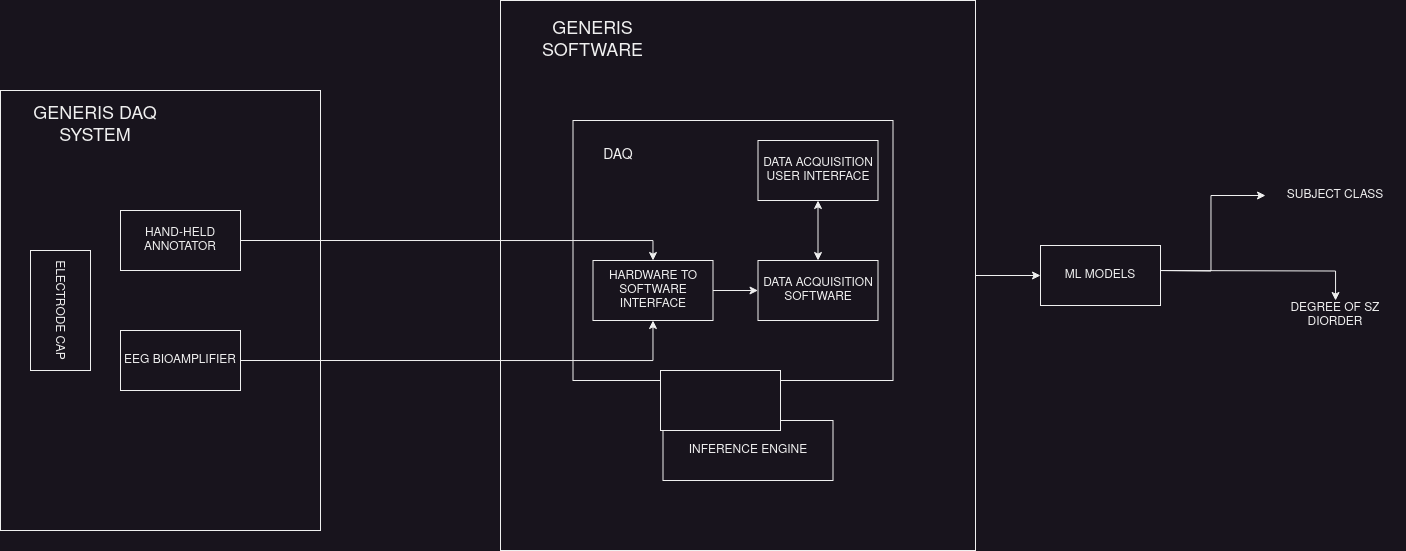
\includegraphics[width=16cm]{../../../images/technical/instrument.drawio.png}
  \caption{\gls{sz} diagnosis instrument}\label{instrument}
\end{figure}


\section{Handheld clicker}
The handheld clicker design is based on an arduino nano which applies the output of four 
tact switches as inputs to four vectored interrupts on the nano development board. The 
exact labels of these inputs has not been assigned as a study of the erogonomics of 
conventions employed in other devices of this kind and how best conventions are adapted and 
modified for the use case of this project is being studied. 

The current design of the handheld clicker(annotator) is the second iteration and is referred 
to as HC-v0.2. 
The circuit diagram of the handheld clicker is given in figure \ref{clicker_circuit}.
The flowchart describing the algorithm of this device is shown in figure \ref{clicker_flowchart}. 
The front and top images of the hand-clicker-v0.2 are shown in figures \ref{clicker} and 
\ref{top_view_of_clicker}.
\begin{figure}[H]
  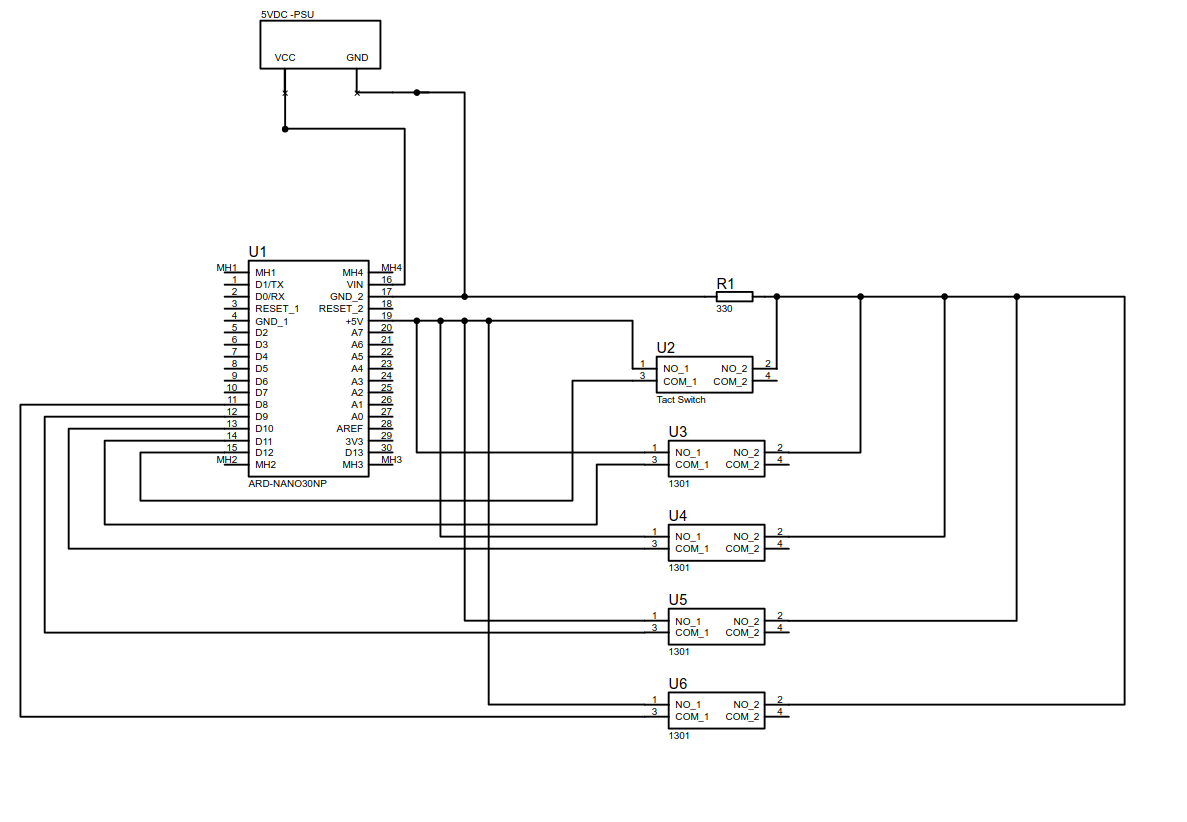
\includegraphics[width=16cm]{../../../hardware/handheld_clicker/circuit_image.png}
  \caption{handheld clicker circuit}\label{clicker_circuit}
\end{figure}
\begin{figure}[H]
  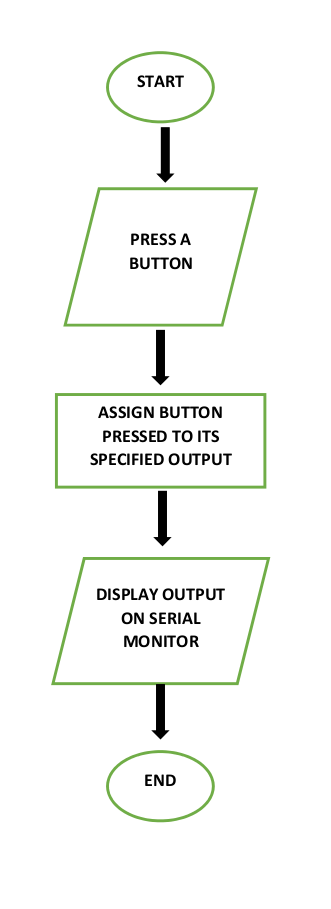
\includegraphics[height=16cm,width=10cm]{../../../hardware/handheld_clicker/flowchart.png}
  \caption{Flowchart algorithm of clicker}\label{clicker_flowchart}
\end{figure}
\begin{figure}[H]
  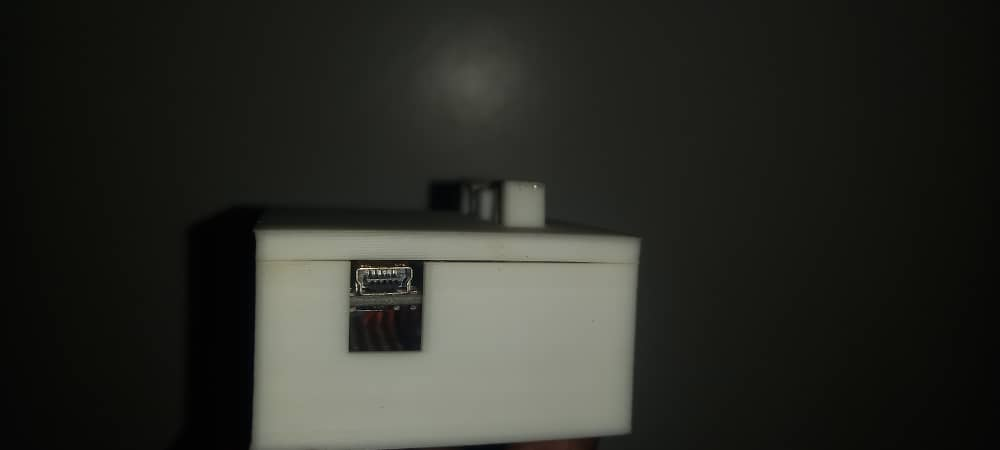
\includegraphics[width=16cm]{../../../hardware/handheld_clicker/front.jpeg}
  \caption{Front view of clicker}\label{clicker}
\end{figure}
\begin{figure}[H]
  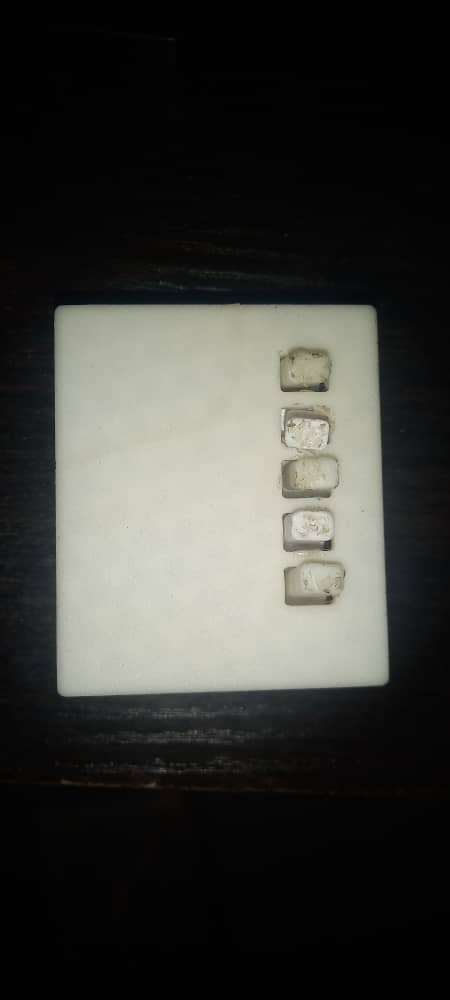
\includegraphics[,height=10cm,width=8cm]{../../../hardware/handheld_clicker/top.jpeg}
  \caption{Top view of clicker}\label{top_view_of_clicker}
\end{figure}


\section{Model Development (Feature-extraction, Data-analysis)}
\subsection{Feature Extraction}
March's report presented the fuzzy entropy features extracted from cortical
regions during phases of \gls{daq} and also the refined \gls{mmn} plots which 
made the \gls{mmn} waveform more evident. Relevant changes made to features 
extraction highlighted in marchs's report includes:
\begin{itemize}
  \item Recomputing the \gls{mmn} waveforms
  \item Spatial dimension augmentation with gaussian noise during computation of fuzzy-entropy
  \item Development of custom fuzzy-entropy library
\end{itemize}
The following was proposed as the next set of action points:
\begin{itemize}
  \item The continued improvement of fuzzy-entropy library to work with multivariate \\
  time-series(2D data)
  \item comparing performance of the fuzzy-entropy features from sourced library to \\
  that of the personally developed library
  \item Computing the auditory steady state features
\end{itemize}
A slight detour was made from these proposed action points for the month of april. 
Analysis of the extracted features for levels of dicriminability was carried out 
to understand how to improve the features extraction methods. The analysis shows 
a significant level of discrimination in the \gls{mmn} features, less in the 
fuzzy-entropy features, though the correlation patterns of the fuzzy-entropy features 
suggest they might carry information on extent of \gls{sz} disorder.

\gls{mmn} features have been extracted from the scaled \gls{mmn} waveforms. The 
\gls{mmn} features were computed as the mean of the \gls{mmn} waveforms within 
the time-frames 0-100ms, 100-200ms, 200-300ms, 300-400ms, 400-450ms.

Formerly implemented montage plot algorithm was improved upon to reduce 
time-complexity so as to make data visualization and analysis easier to obtain 
intuitive information from.

\subsection{Data Analysis/Visualization}\label{data_analyis}
 Analysis of the extracted features was done to establish the quality of discriminative 
 and quantitative information contained in the extracted features. The method of 
 Visualization of some of these features changed to make analysis easy.
 The results of the analysis are given in section \ref{figures}. Visualization methods 
 and analysis carried out includes:
\begin{itemize}
  \item Comparing \gls{mmn} feature values for 1KHz duration deviant and 3KHz frequency deviant 
  between patient and controls across all electrodes and time windows.
  (Figures \ref{mmnvalue_0_100ms} - \ref{mmnvalue_400_450ms})
  \item Converting the \gls{mmn} values to montage plots for 1KHz duration deviant 
  and 3KHz frequency deviant for easier interpretation and analyzing montage evolution.
  (Figures \ref{control_1KHz_mmn_montage}-\ref{patient_3KHz_mmn_montage})
  \item Comparing distribution of computed fuzzy-entropy values of patients and controls 
  for each cortical region across all phases of \gls{daq}.
  (Figures \ref{fig:controlFuzzEnt}-\ref{fuzz_ent_distributions}) 
  \item Correlating fuzzy-entropy values from cortical regions across 
  all phases of \gls{daq}.(Figure \ref{fuzz_ent_corr_mat})
  \item Comparing entropies from all cortical regions for each phase of \gls{daq}.
  (Figures \ref{rest_fuzz}-\ref{auditory_fuzz})
  \item Comparing entropies from all phases of \gls{daq} for each cortical region.
  (figures \ref{frontal_fuzz}-\ref{temporal_fuzz})
\end{itemize} 

\section{Inference and Action Points}
\subsection{Inference}
From the analysis carried out, the \gls{mmn} features of both tone deviants show 
discriminative properties between the \gls{szPtnt} and \gls{hc} in localized head 
regions. The fuzzy-entropy features do not show discriminative abilities, but their 
correlation patterns indicate a linear relationship that might be a measure of degree 
of \gls{sz} disorder. Therefore we need to find methods that improve quality of extracted 
features and proceed with developing a learner model.

\subsection{Action Points}
Based on the inference drawn, the action points for the month of may is as follows:
\begin{itemize}
  \item Computing the auditory steady state features.
  \item Re-computing fuzzy-entropy features using other libraries and 
  comparing performance.
  \item Improve discriminability of features using spatial filters and dimensionality 
  reduction techniques.
  \item Compare performance of a custom mutilayer feedforward network and traditional 
  machine-learning algorithms for classification and estimation of measures of degree 
  of \gls{sz} disorder.
\end{itemize}

\section{Figures}\label{figures}

\begin{figure}[H]
  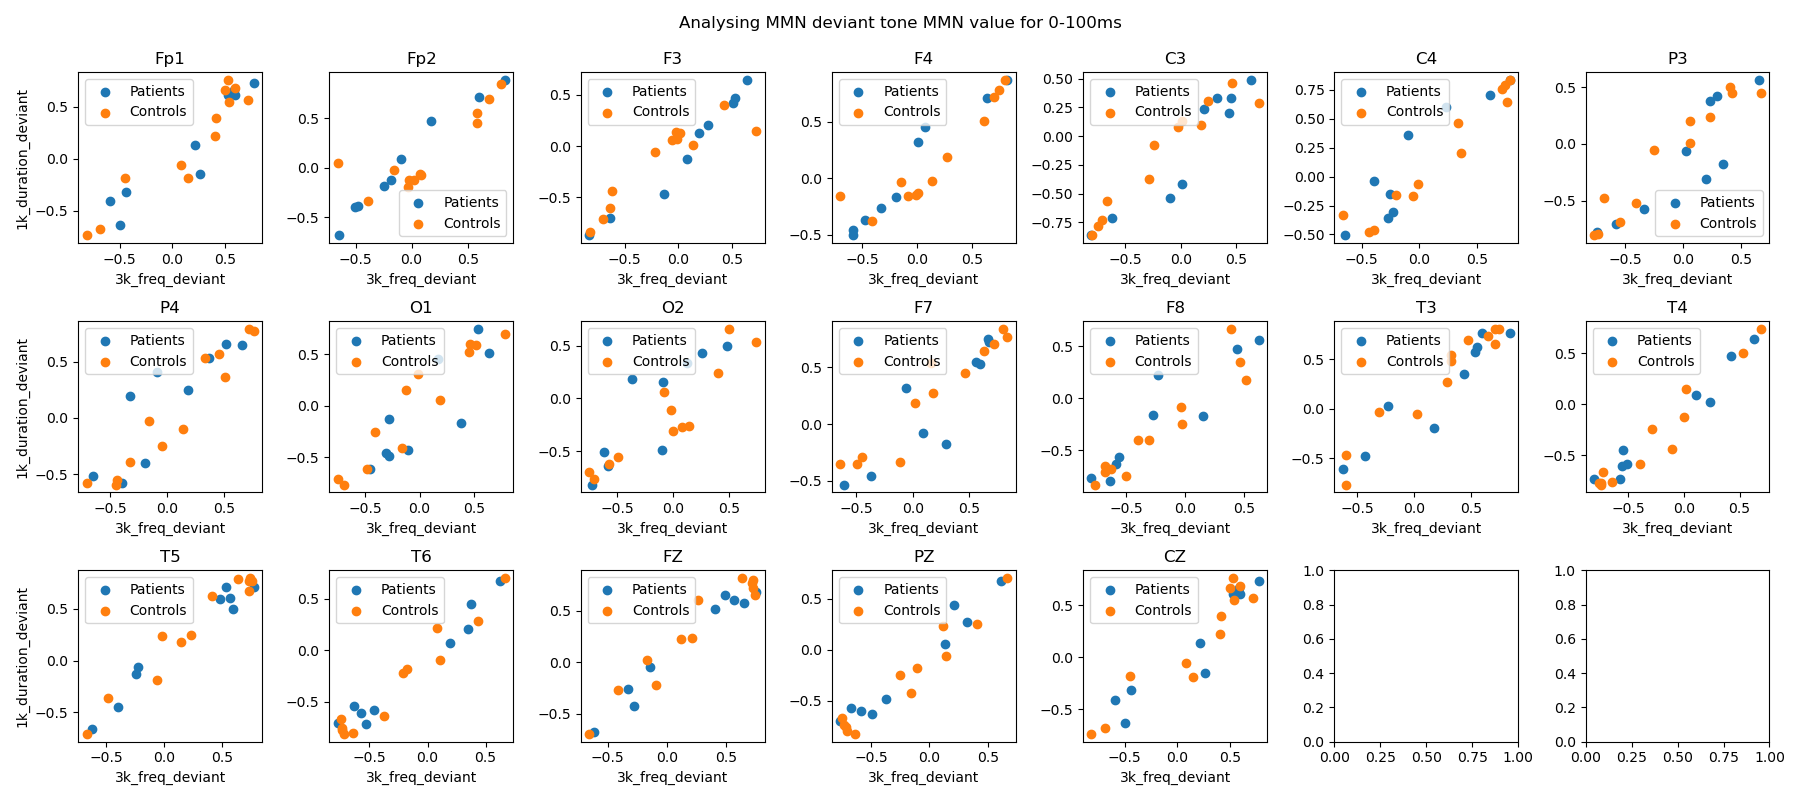
\includegraphics[width=16cm]{../../../data_analysis_results/MMN/features/deviant_tone_0.png}
  \caption{\gls{mmn} values from 0-100ms}\label{mmnvalue_0_100ms}
\end{figure}
\begin{figure}[H]
  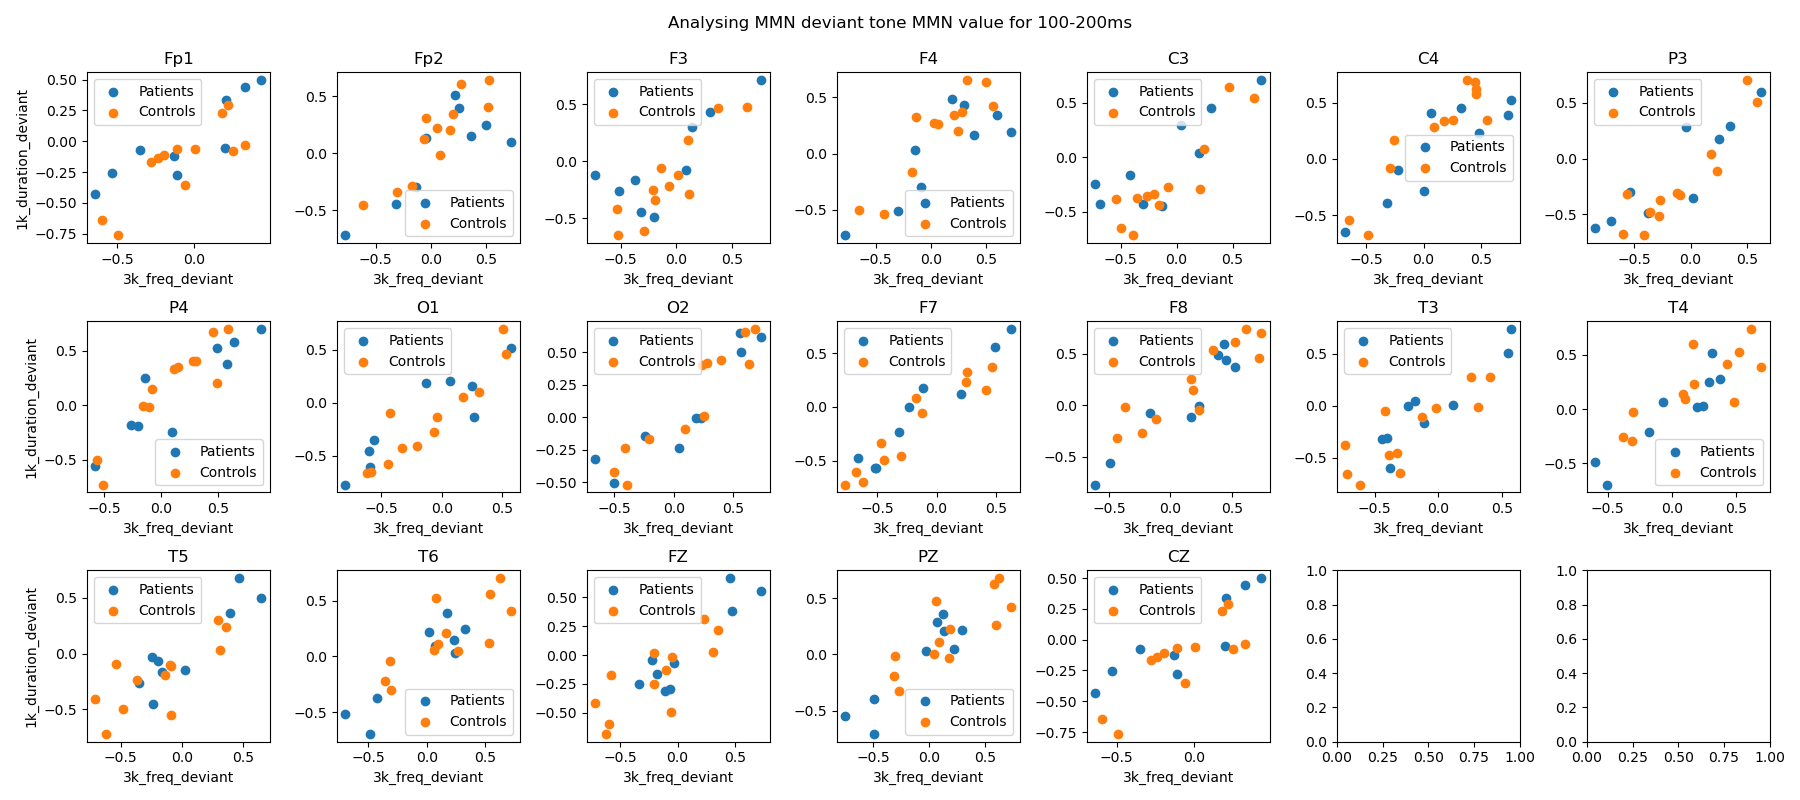
\includegraphics[width=16cm]{../../../data_analysis_results/MMN/features/deviant_tone_1.png}
  \caption{\gls{mmn} values from 100-200ms}\label{mmnvalue_100_200ms}
\end{figure}
\begin{figure}[H]
  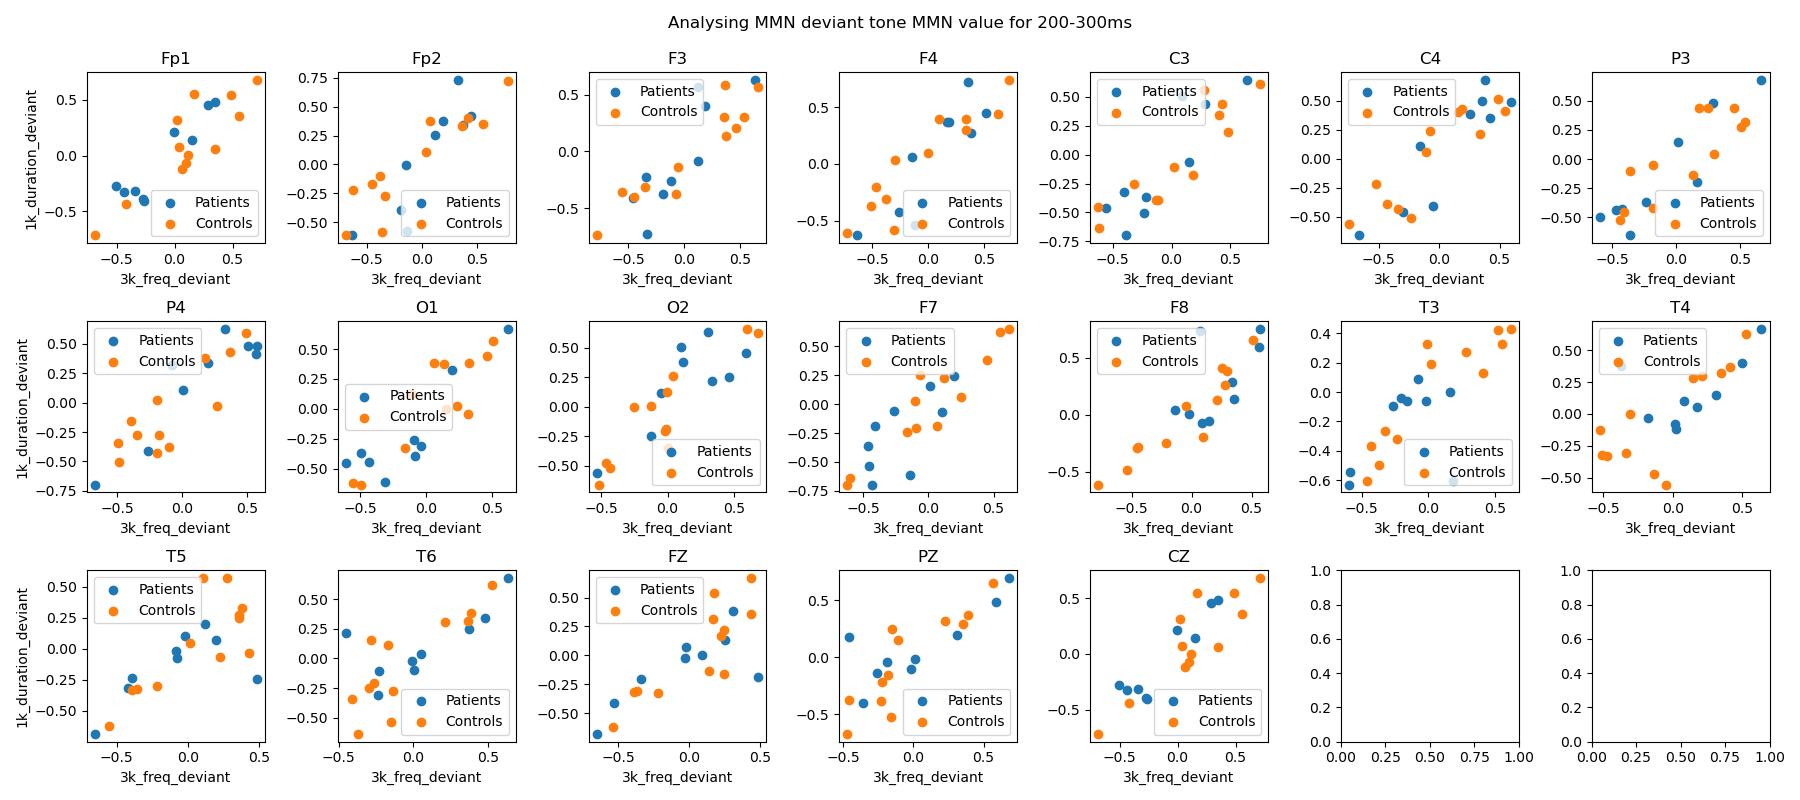
\includegraphics[width=16cm]{../../../data_analysis_results/MMN/features/deviant_tone_2.png}
  \caption{\gls{mmn} values from 200-300ms}\label{mmnvalue_200_300ms}
\end{figure}
\begin{figure}[H]
  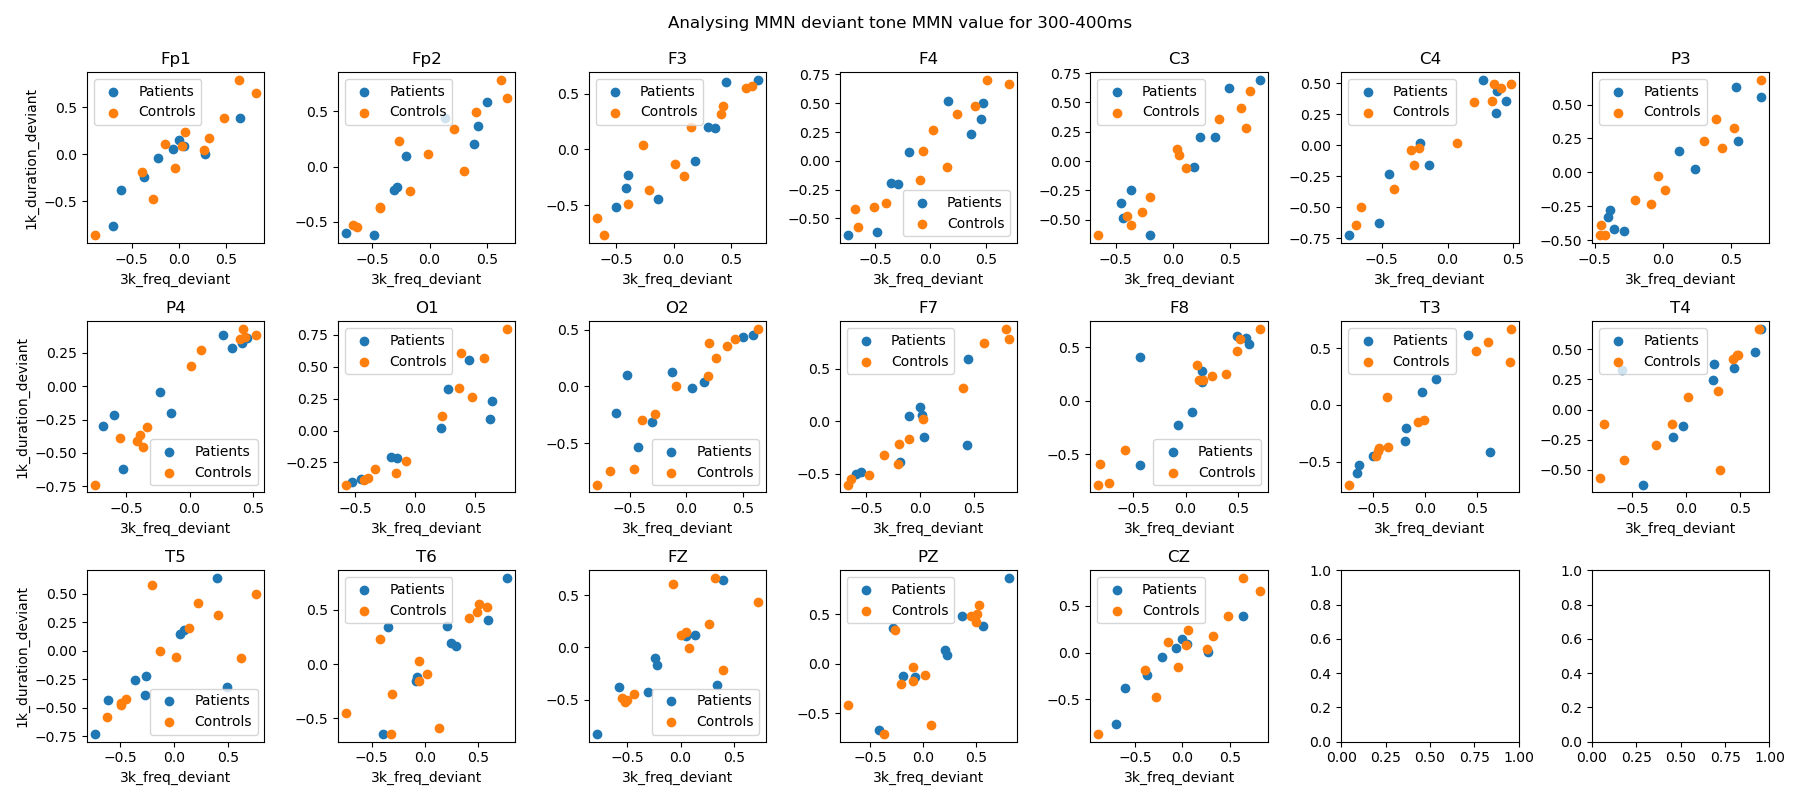
\includegraphics[width=16cm]{../../../data_analysis_results/MMN/features/deviant_tone_3.png}
  \caption{\gls{mmn} values from 300-400ms}\label{mmnvalue_300_400ms}
\end{figure}
\begin{figure}[H]
  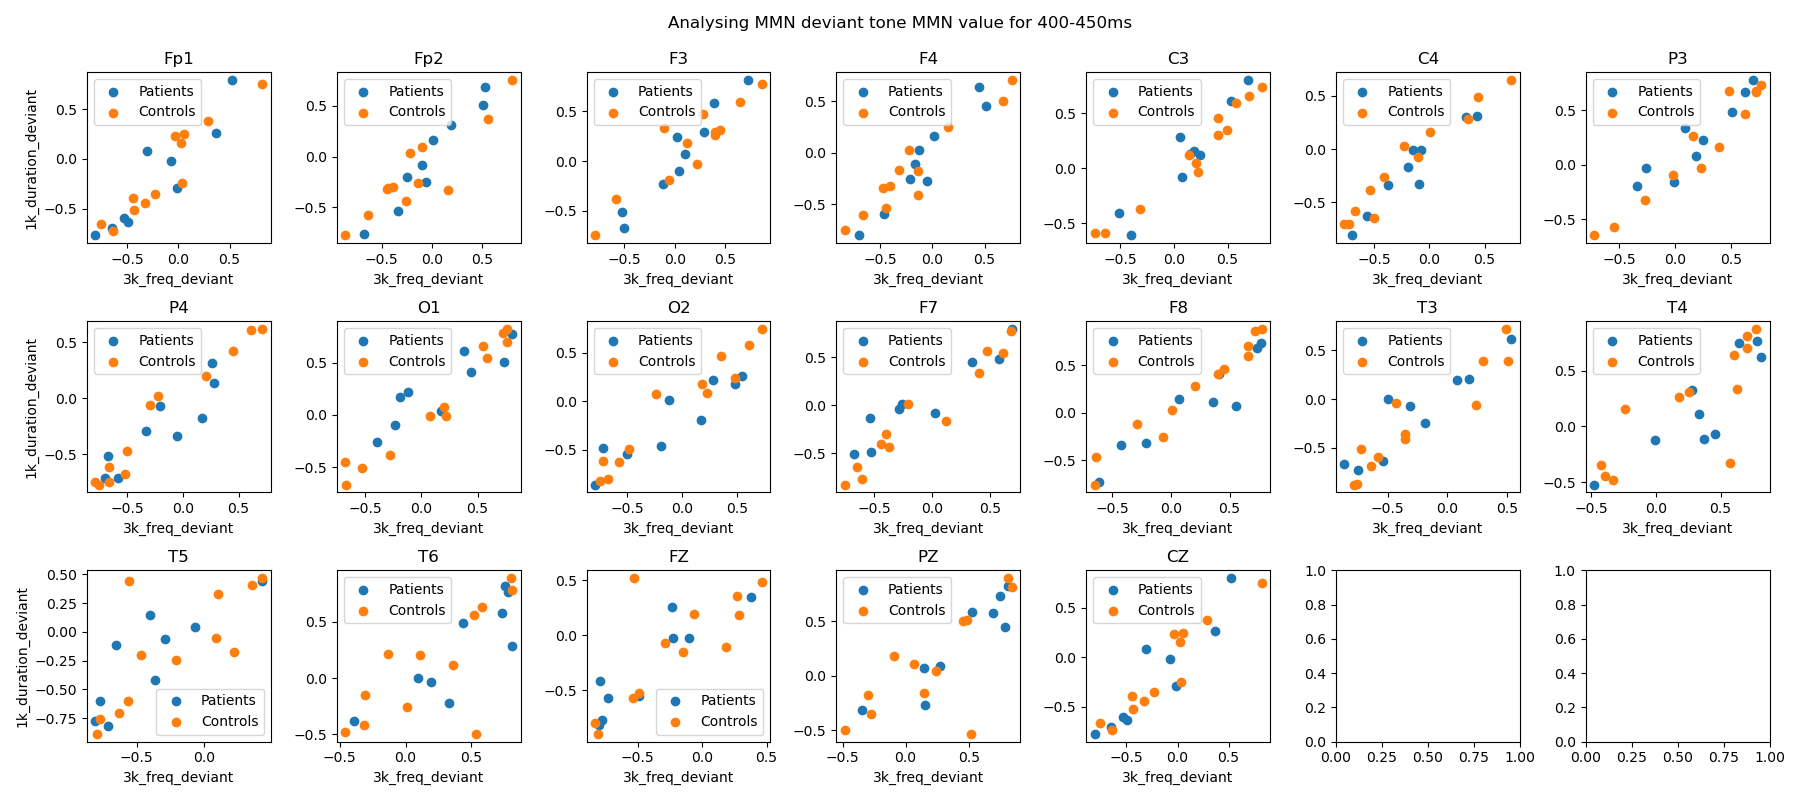
\includegraphics[width=16cm]{../../../data_analysis_results/MMN/features/deviant_tone_4.png}
  \caption{\gls{mmn} values from 400-450ms}\label{mmnvalue_400_450ms}
\end{figure}

\begin{figure}[H]
  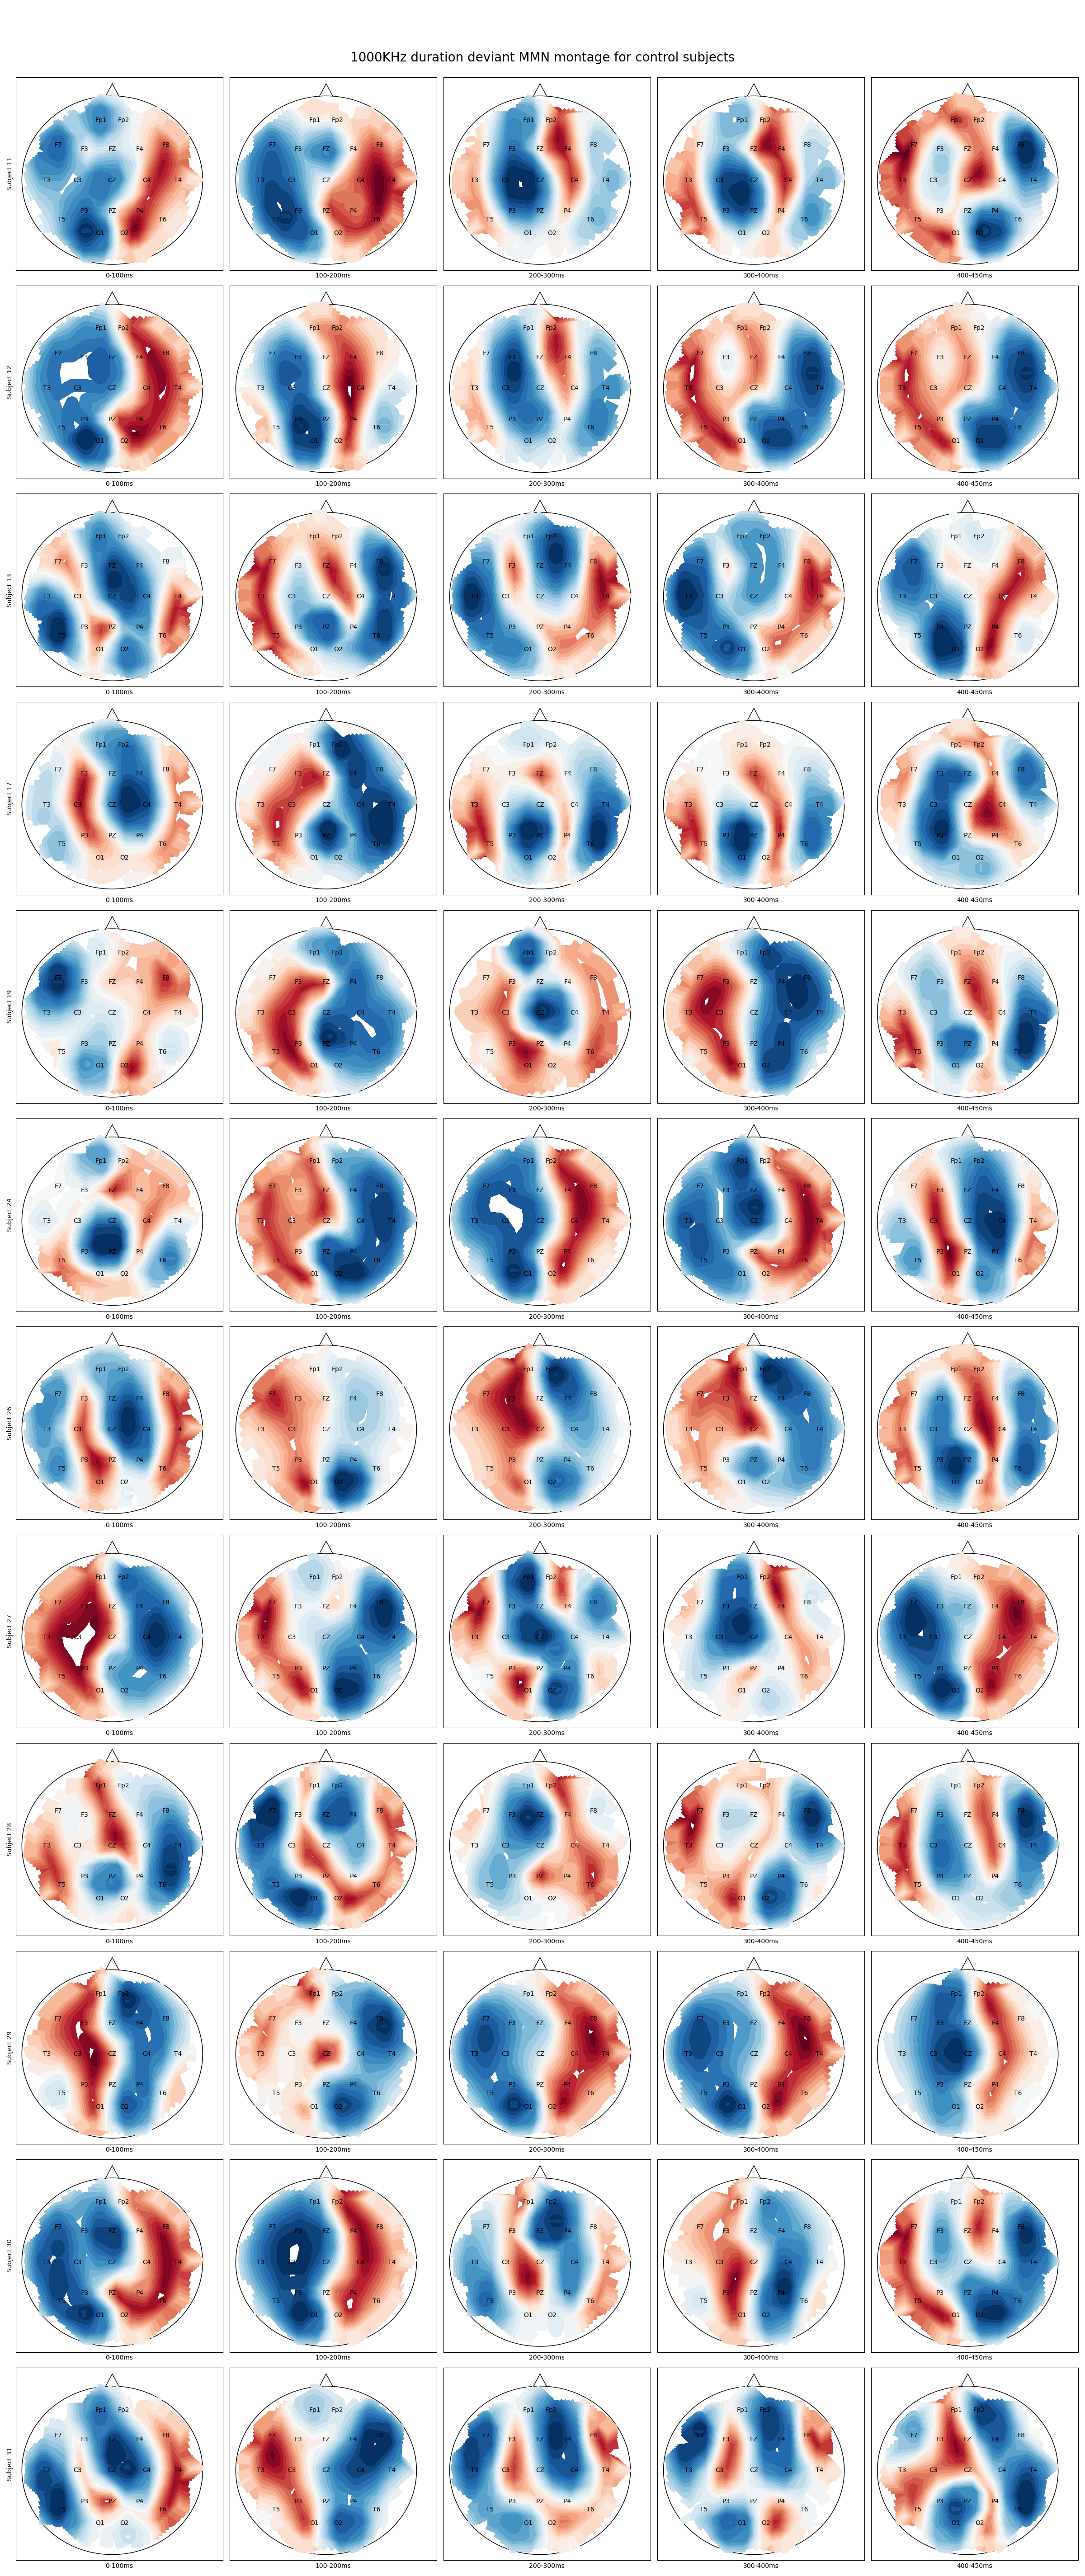
\includegraphics[width=16cm]{../../../data_analysis_results/MMN/montage/Control/1KHz_duration_deviant_montage.png}
  \caption{Controls 1KHz duration deviant \gls{mmn} value montage}\label{control_1KHz_mmn_montage}
\end{figure}
\begin{figure}[H]
  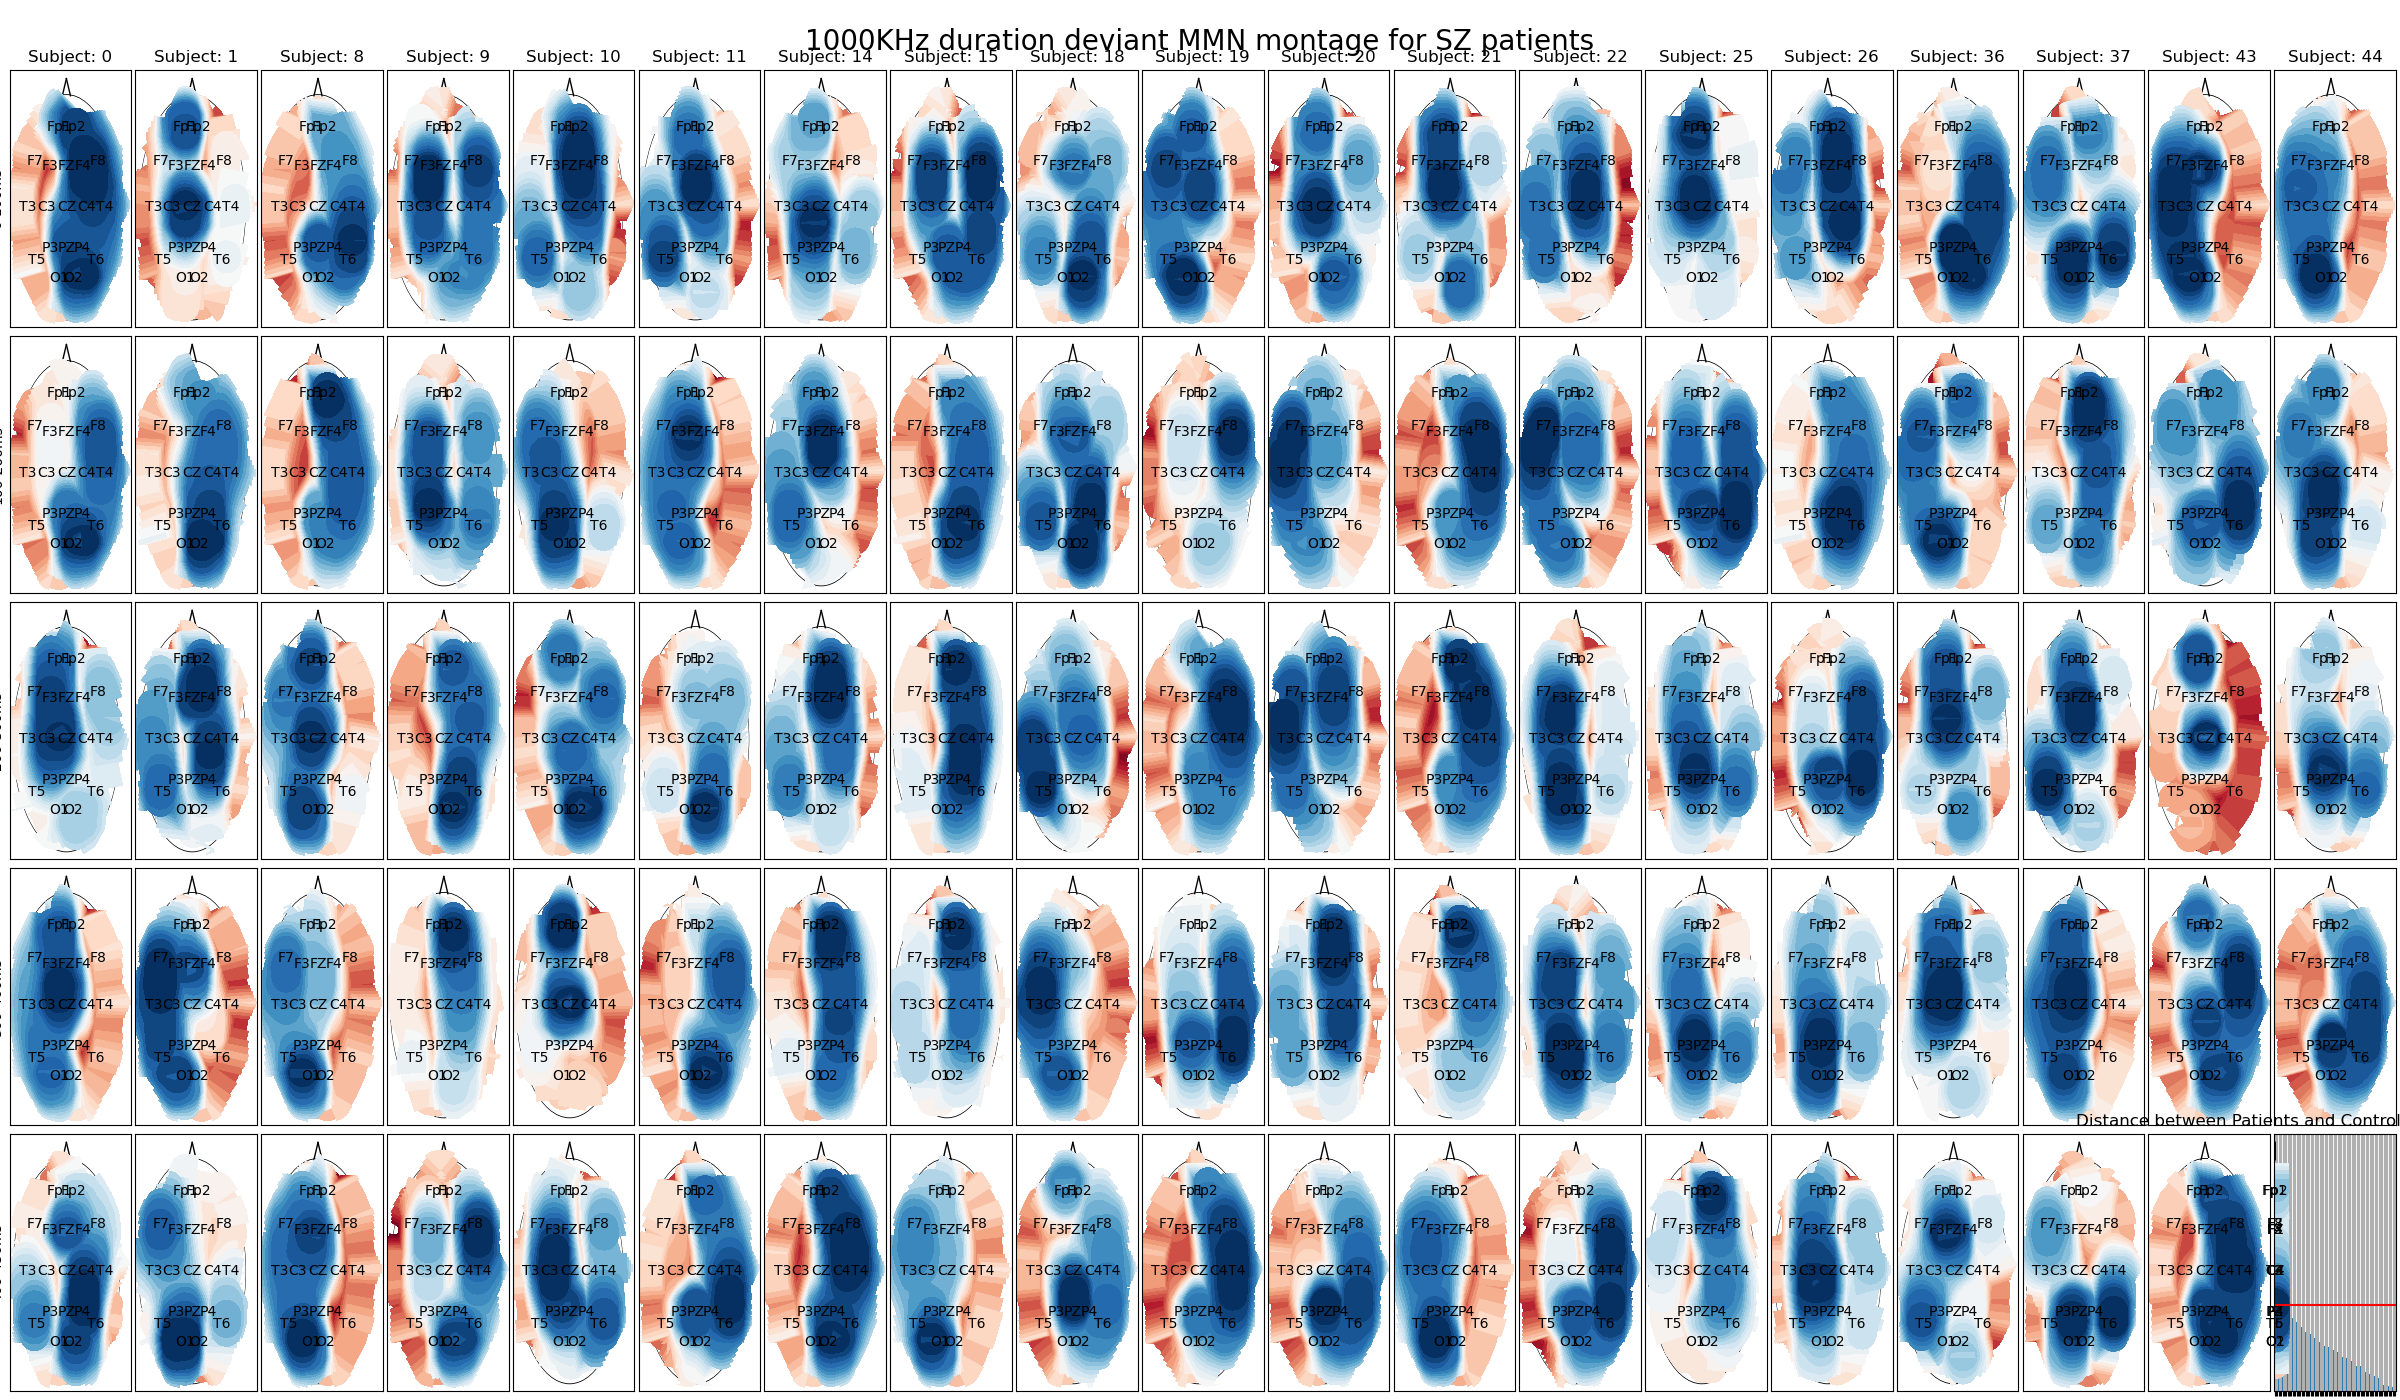
\includegraphics[width=16cm]{../../../data_analysis_results/MMN/montage/Patient/1KHz_duration_deviant_montage.png}
  \caption{Patients 1KHz duration deviant \gls{mmn} value montage}\label{patient_1KHz_mmn_montage}
\end{figure}
\begin{figure}[H]
  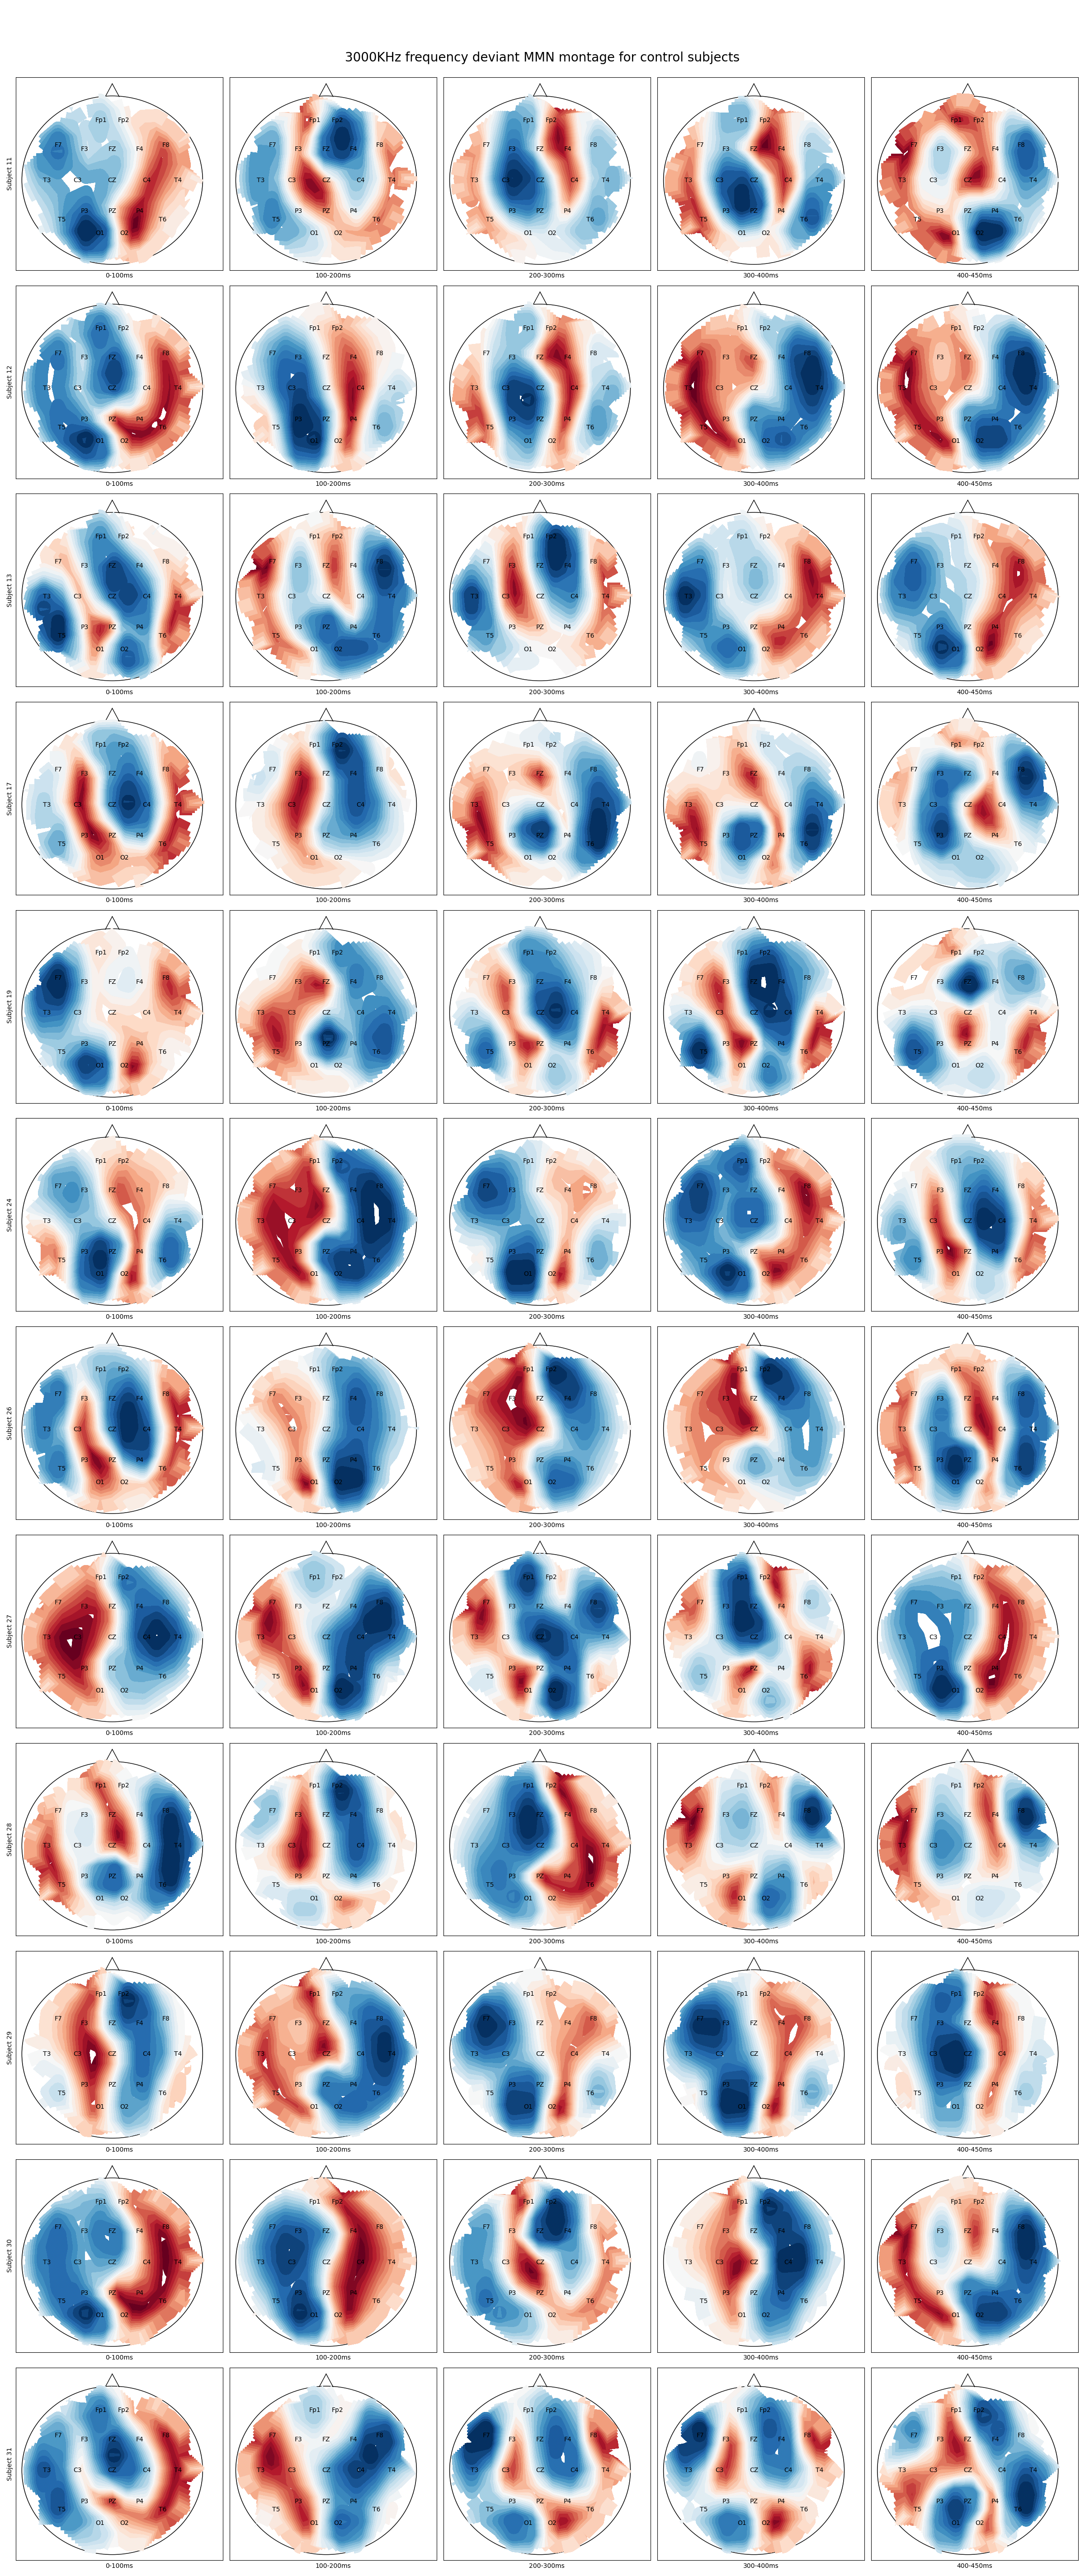
\includegraphics[width=16cm]{../../../data_analysis_results/MMN/montage/Control/3KHz_frequency_deviant_montage.png}
  \caption{Controls 3KHz frequency deviant \gls{mmn} value montage}\label{control_3KHz_mmn_montage}
\end{figure}
\begin{figure}[H]
  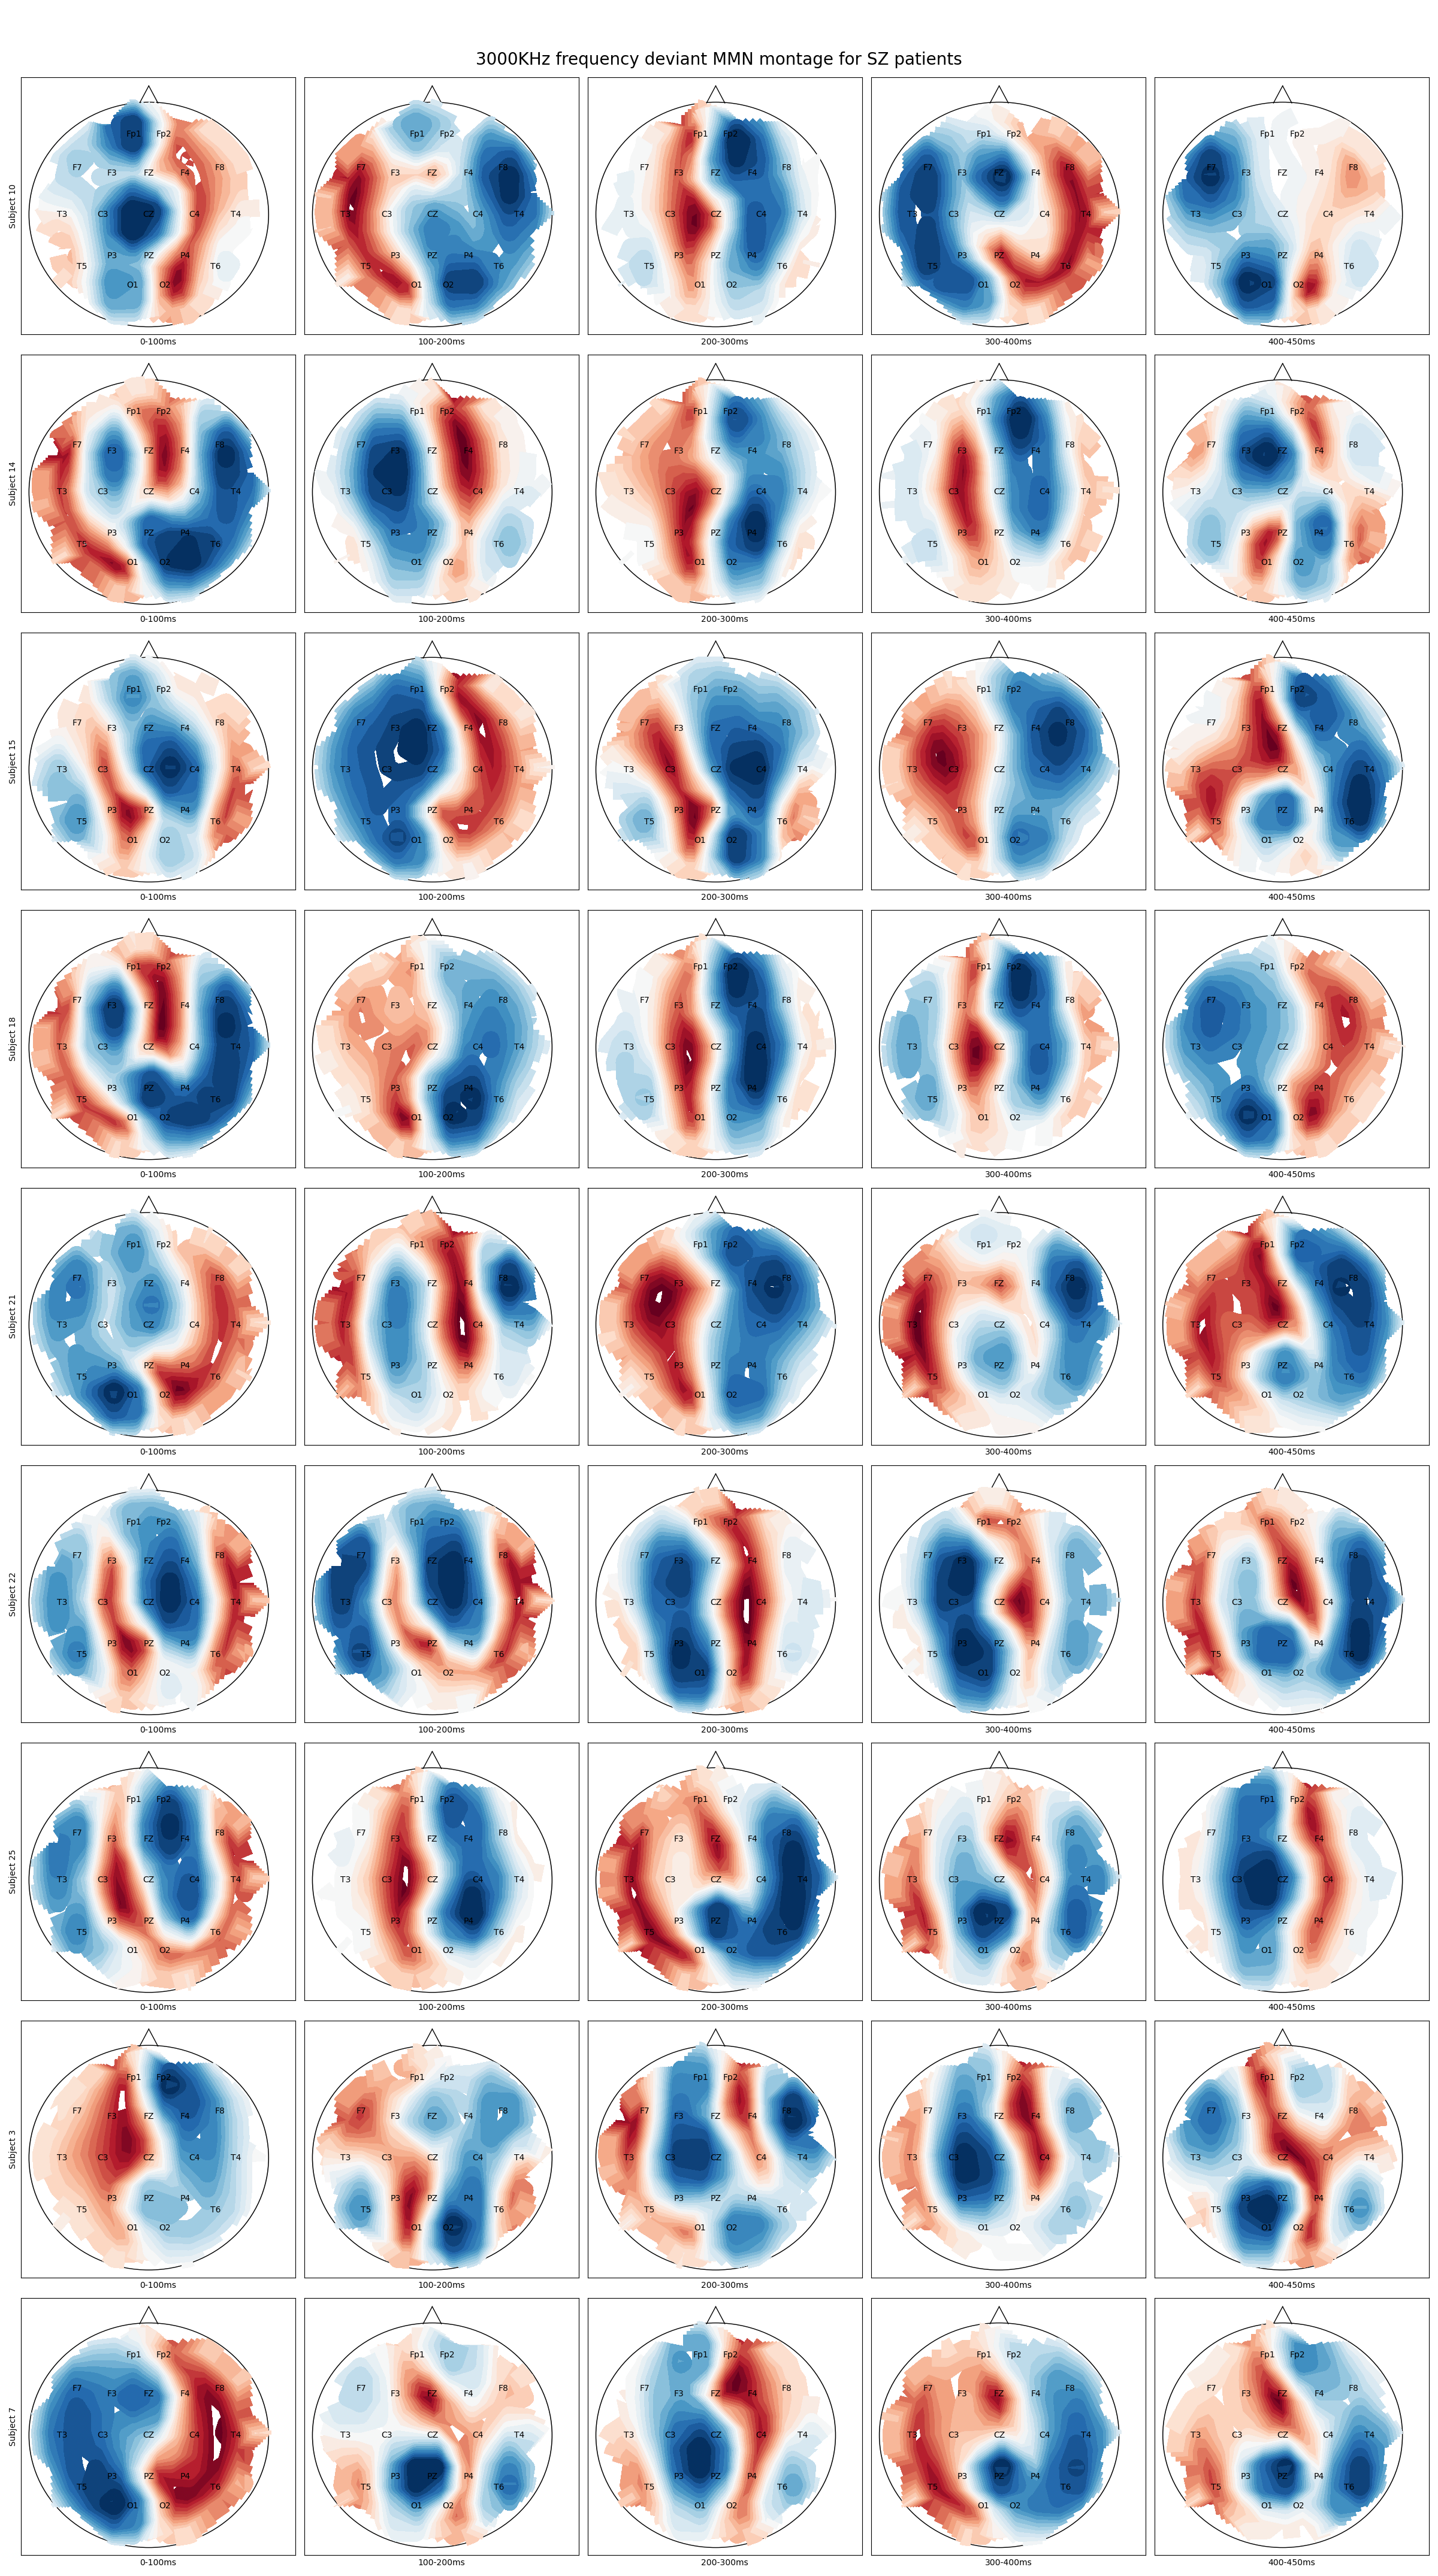
\includegraphics[width=16cm]{../../../data_analysis_results/MMN/montage/Patient/3KHz_frequency_deviant_montage.png}
  \caption{Patients 3KHz frequency deviant \gls{mmn} value montage}\label{patient_3KHz_mmn_montage}
\end{figure}

\begin{figure}[H]
  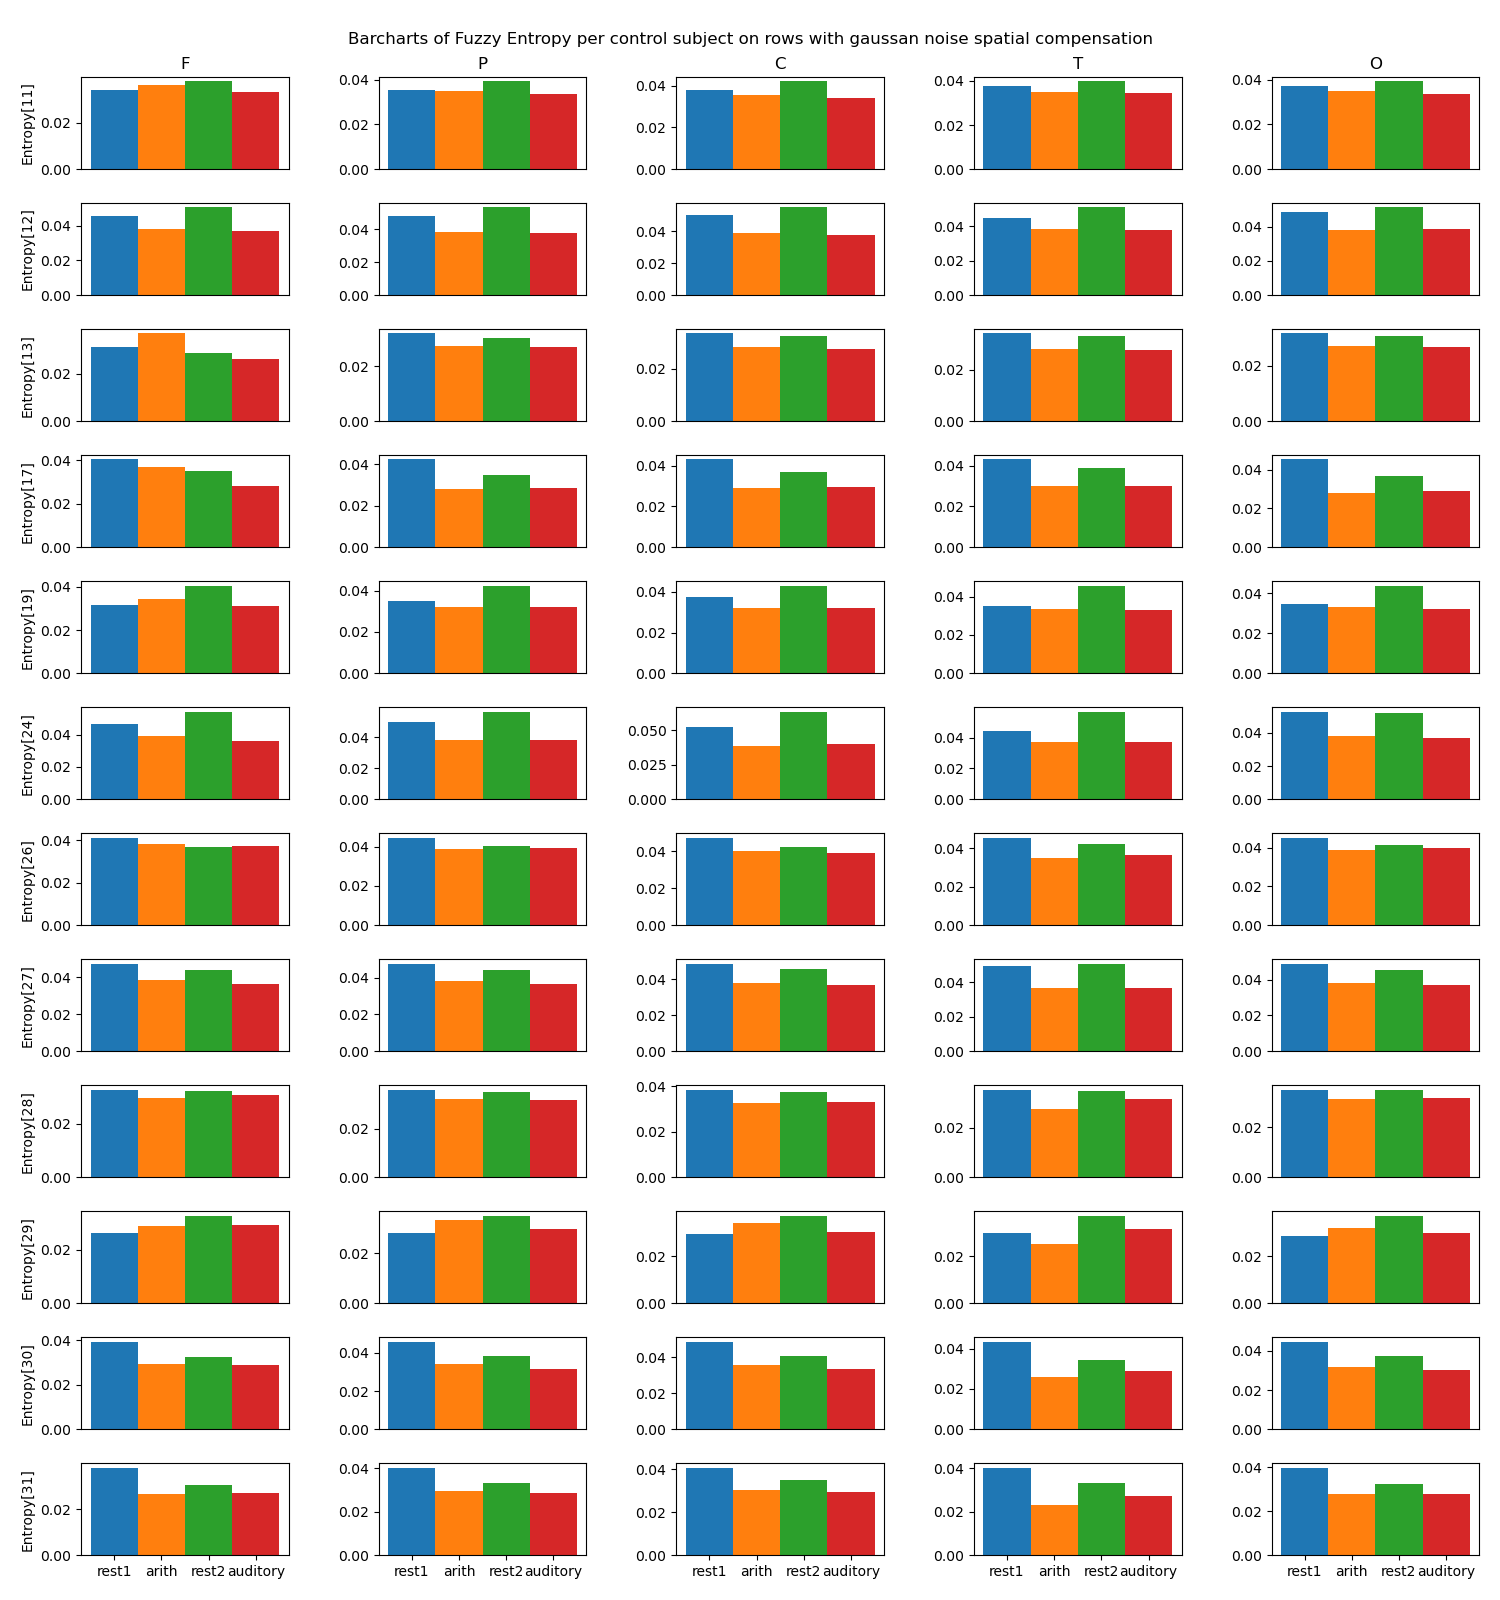
\includegraphics[width=16cm]{../../../data_analysis_results/FuzzEnt/Control/all-fuzzyEntr.png}
  \caption{Fuzzy Entropy from controls}\label{fig:controlFuzzEnt}
\end{figure}
\begin{figure}[H]
  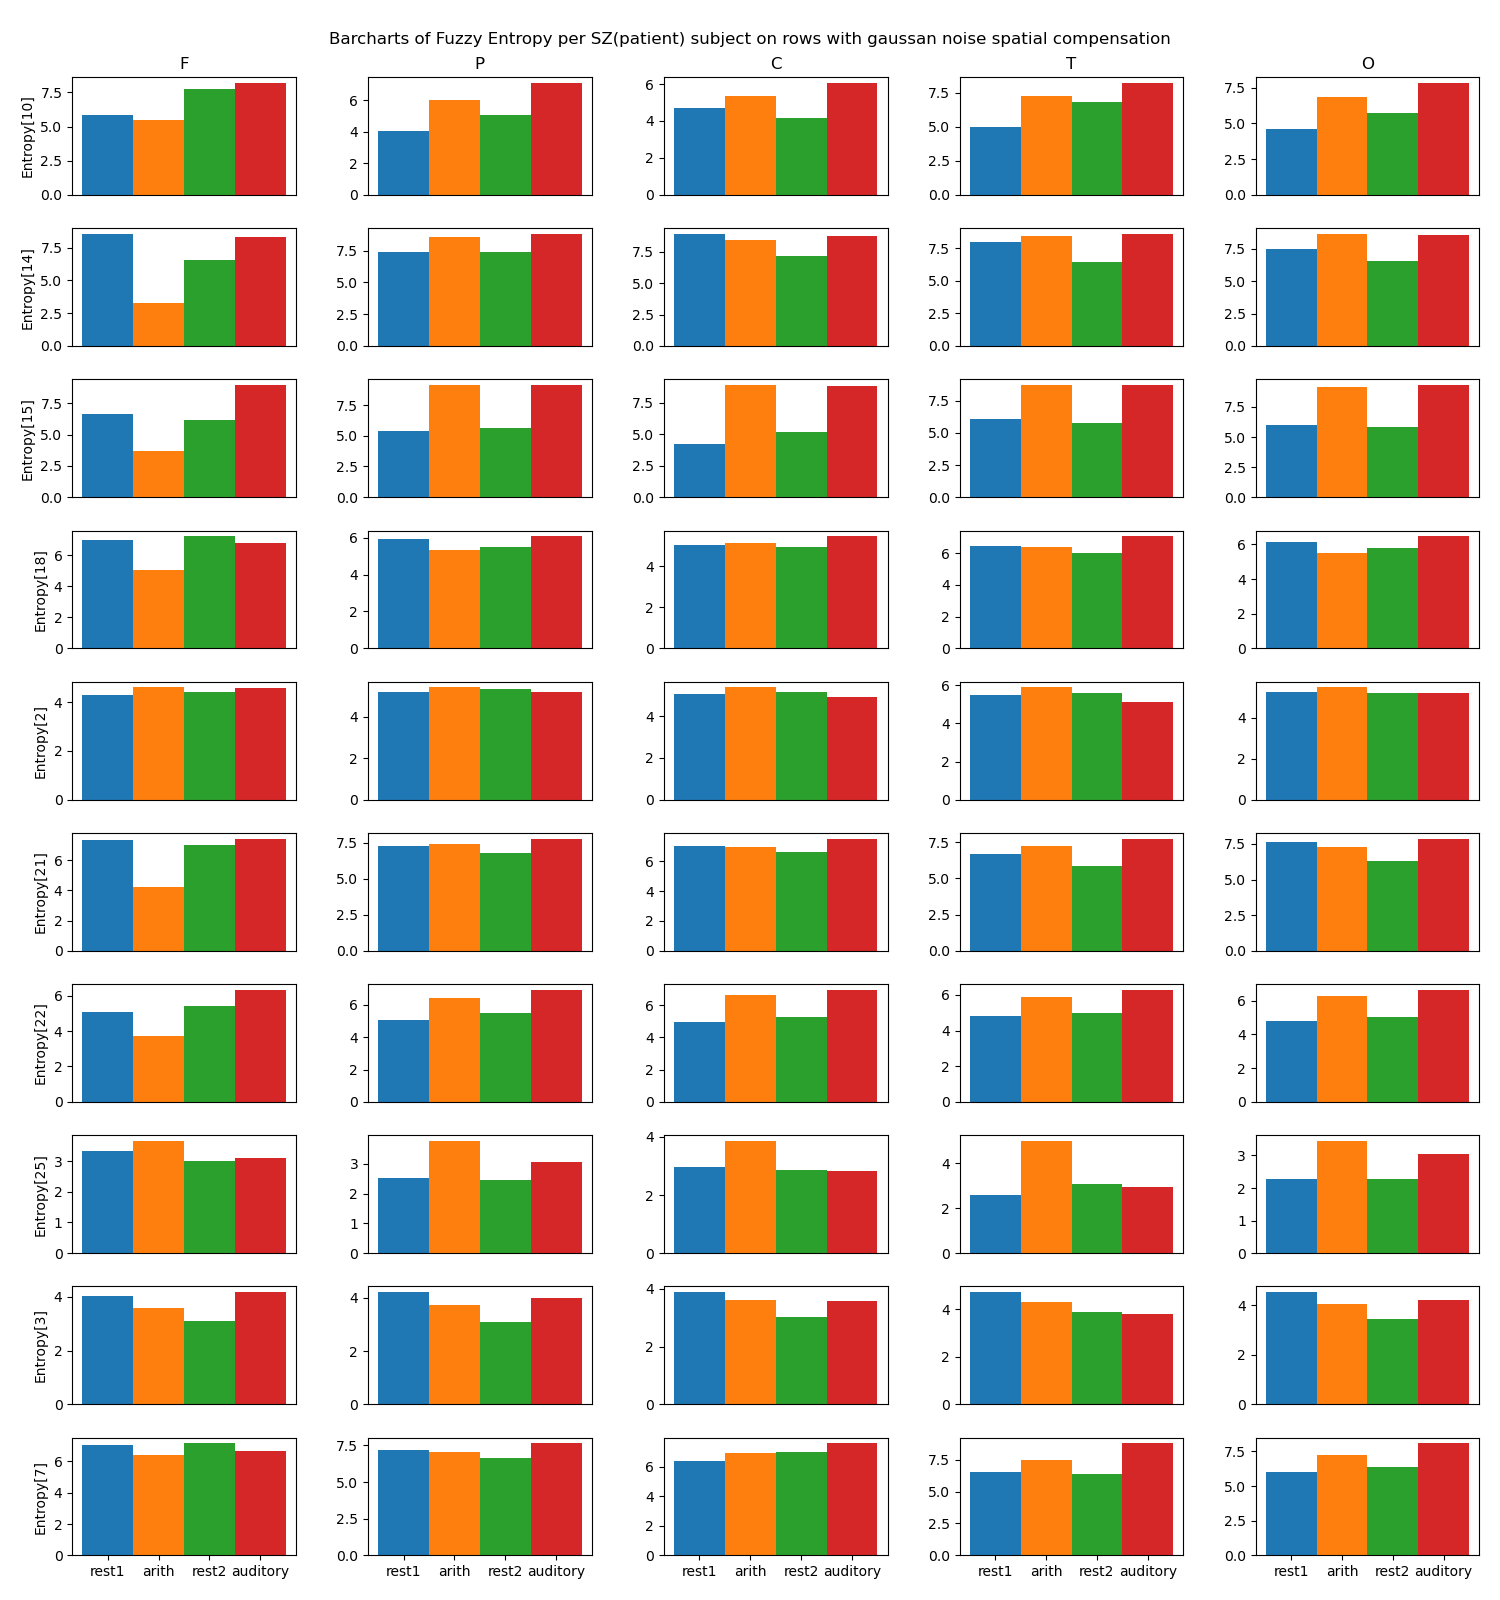
\includegraphics[width=16cm]{../../../data_analysis_results/FuzzEnt/Patient/all-fuzzyEntr.png}
  \caption{Fuzzy Entropy from patients}\label{fig:patientFuzzEnt}
\end{figure}
\begin{figure}[H]
  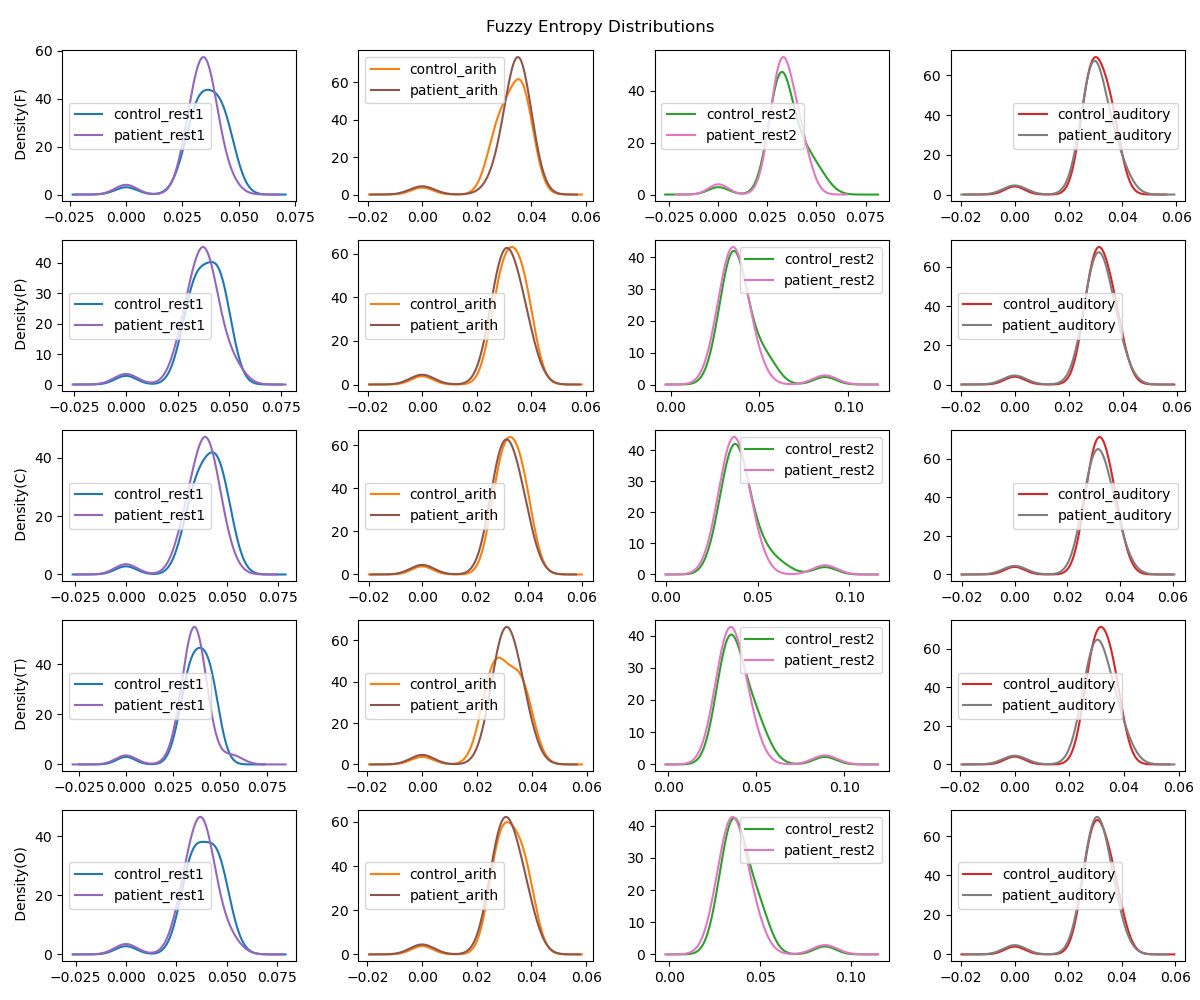
\includegraphics[width=16cm]{../../../data_analysis_results/FuzzEnt/corticalRegions_DAQphase_distributions.png}
  \caption{Fuzzy Entropy from controls}\label{fuzz_ent_distributions}
\end{figure}

\begin{figure}[H]
  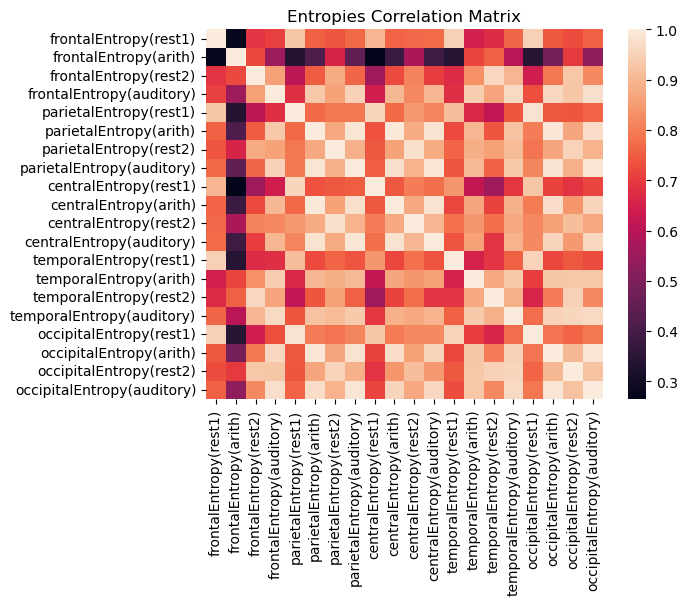
\includegraphics[width=16cm]{../../../data_analysis_results/FuzzEnt/entropies_corr_mat.png}
  \caption{Fuzzy-entropy values correlation smatrix}\label{fuzz_ent_corr_mat}
\end{figure}

\begin{figure}[H]
  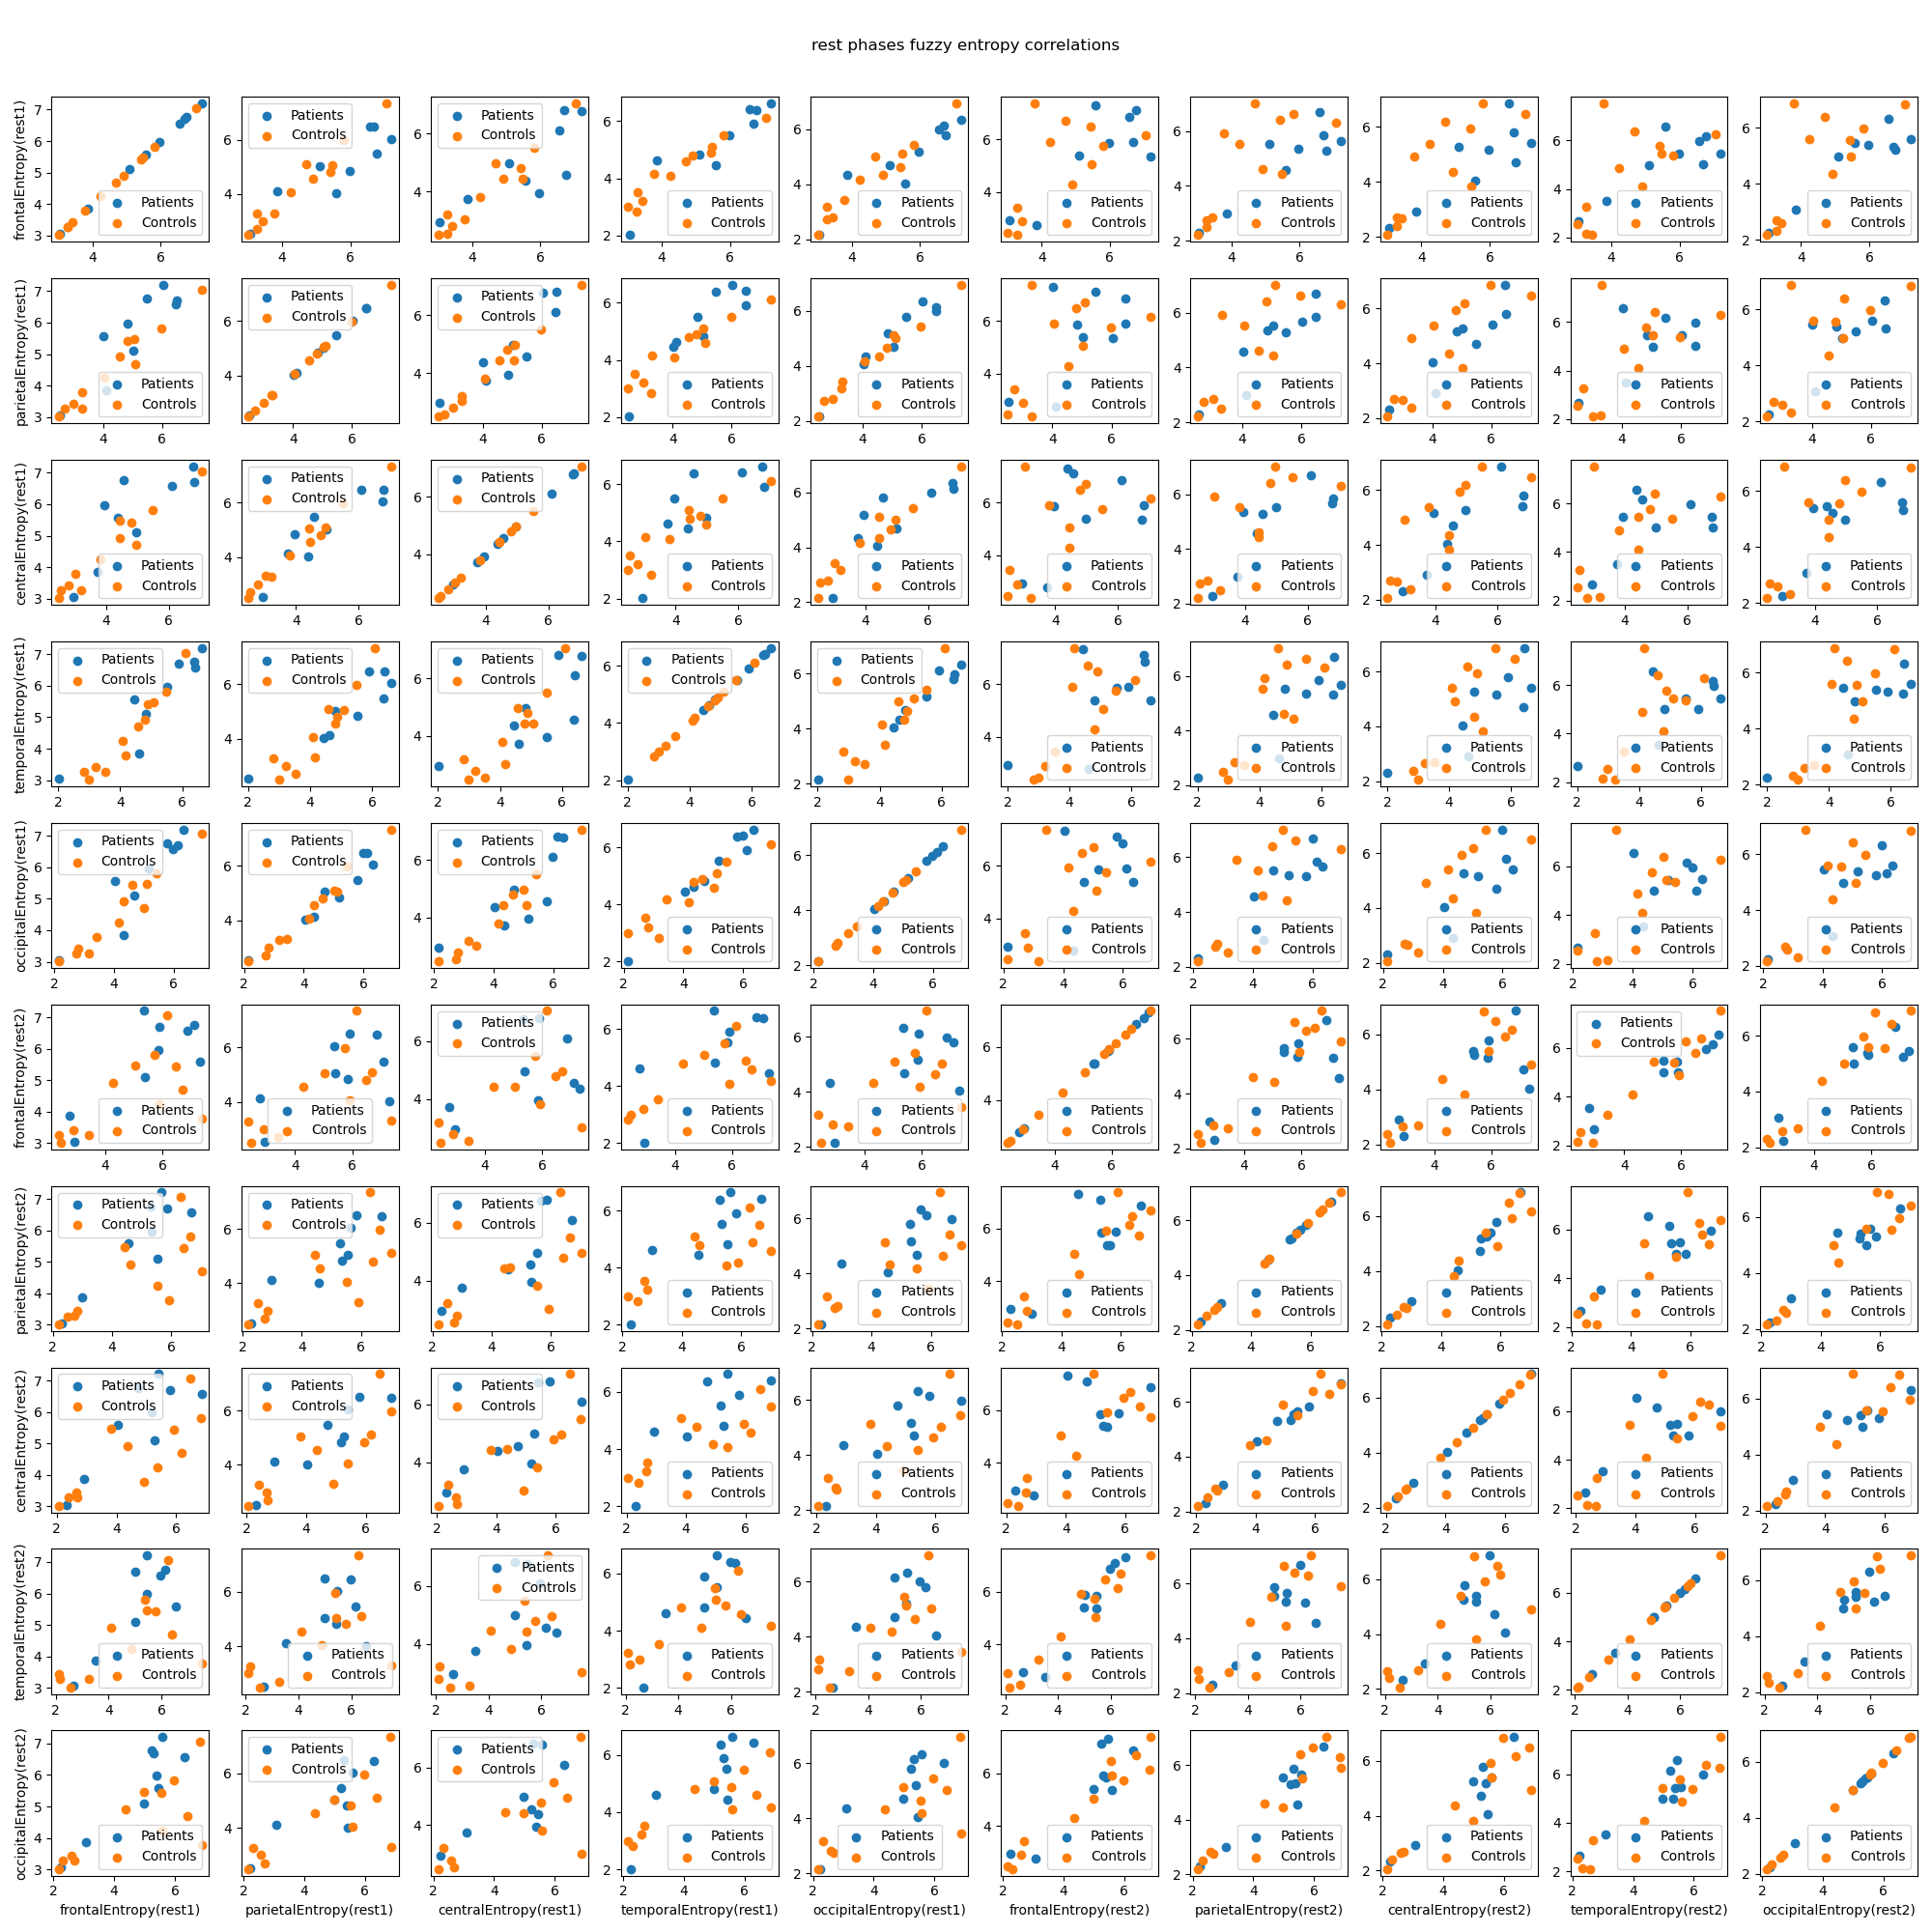
\includegraphics[width=16cm]{../../../data_analysis_results/FuzzEnt/rest_phases_corr.png}
  \caption{Rest Phases Fuzzy-entropy}\label{rest_fuzz}
\end{figure}
\begin{figure}[H]
  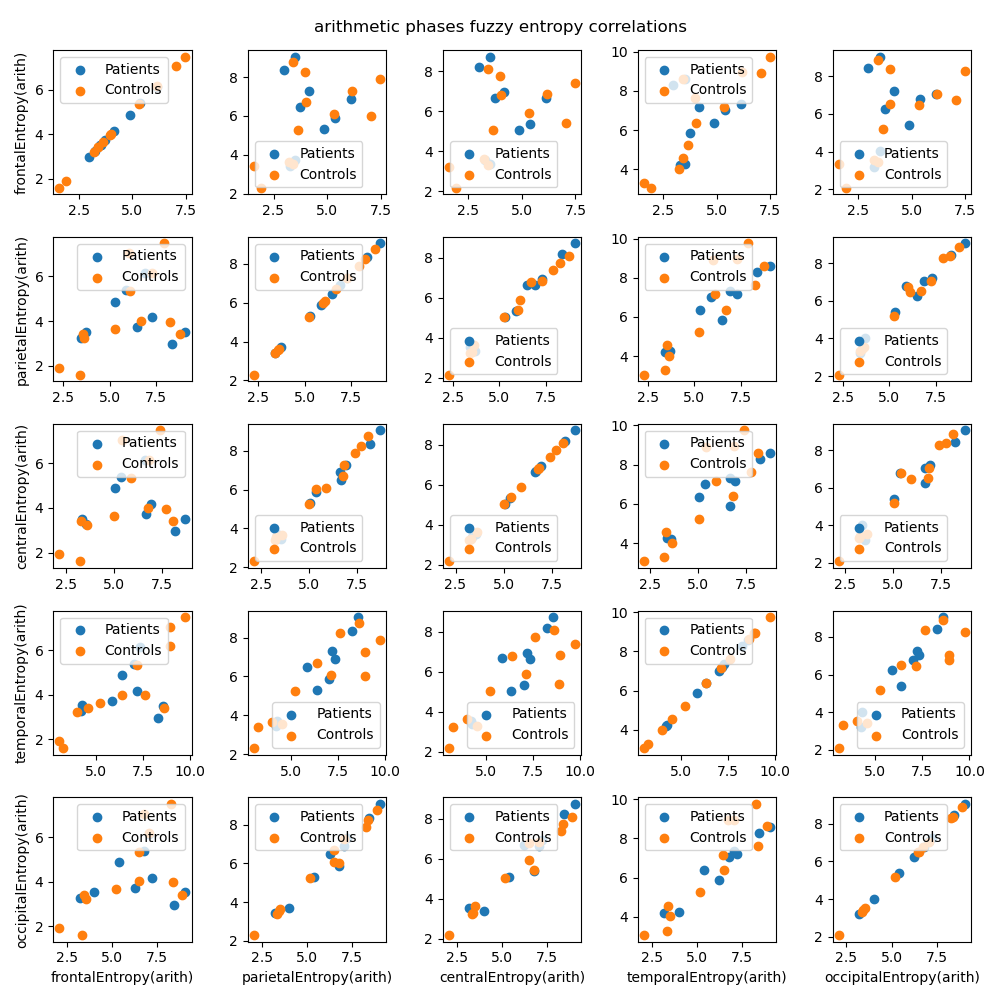
\includegraphics[width=16cm]{../../../data_analysis_results/FuzzEnt/arith_phases_corr.png}
  \caption{Arithmetic Phase Fuzzy-entropy}\label{arith_fuzz}
\end{figure}
\begin{figure}[H]
  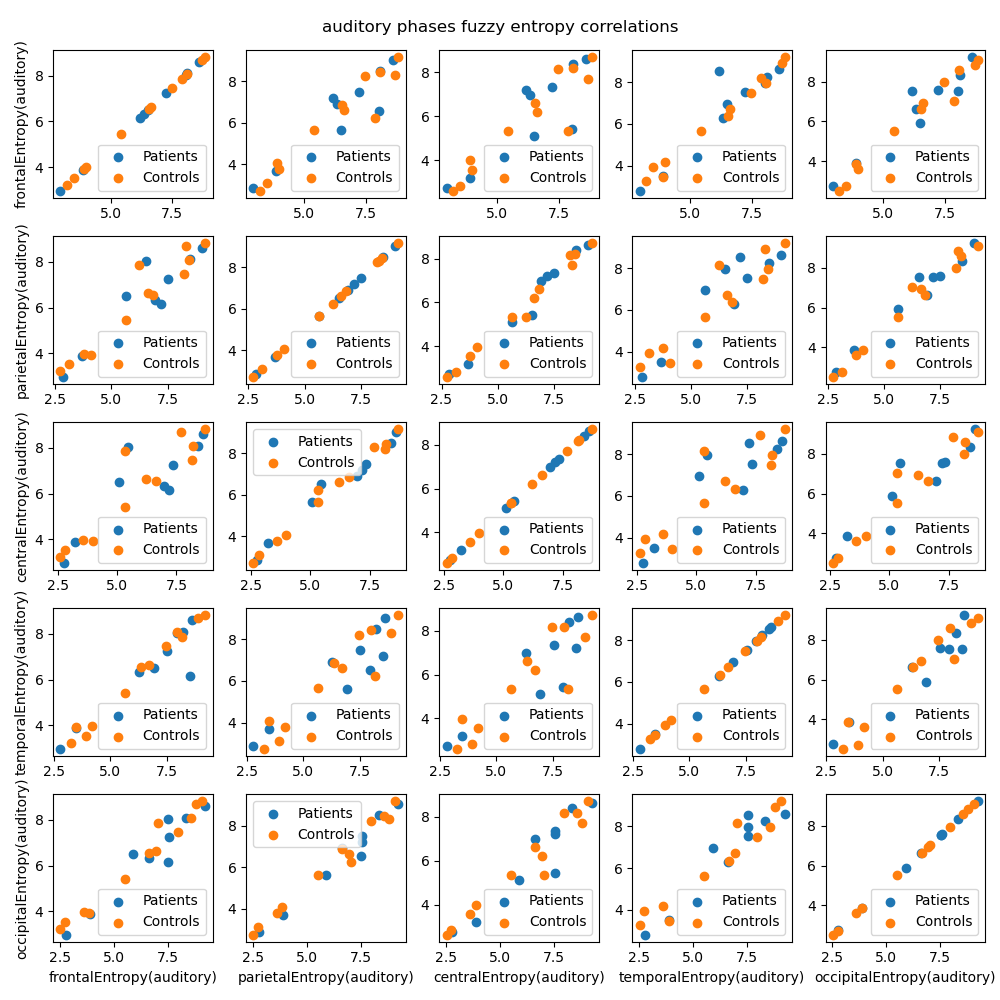
\includegraphics[width=16cm]{../../../data_analysis_results/FuzzEnt/auditory_phases_corr.png}
  \caption{Auditory Phase Fuzzy-entropy}\label{auditory_fuzz}
\end{figure}

\begin{figure}[H]
  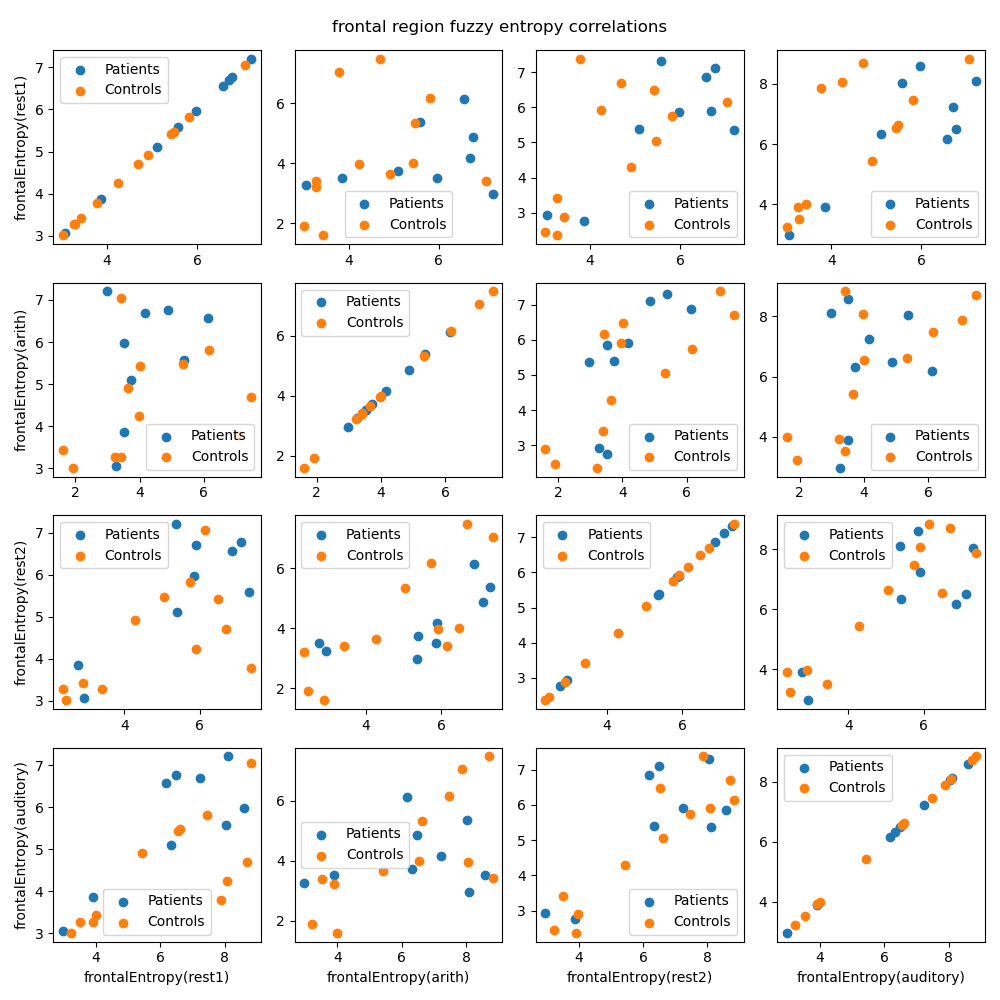
\includegraphics[width=16cm]{../../../data_analysis_results/FuzzEnt/frontal_region_corr.png}
  \caption{Frontal lobe Fuzzy-entropy}\label{frontal_fuzz}
\end{figure}
\begin{figure}[H]
  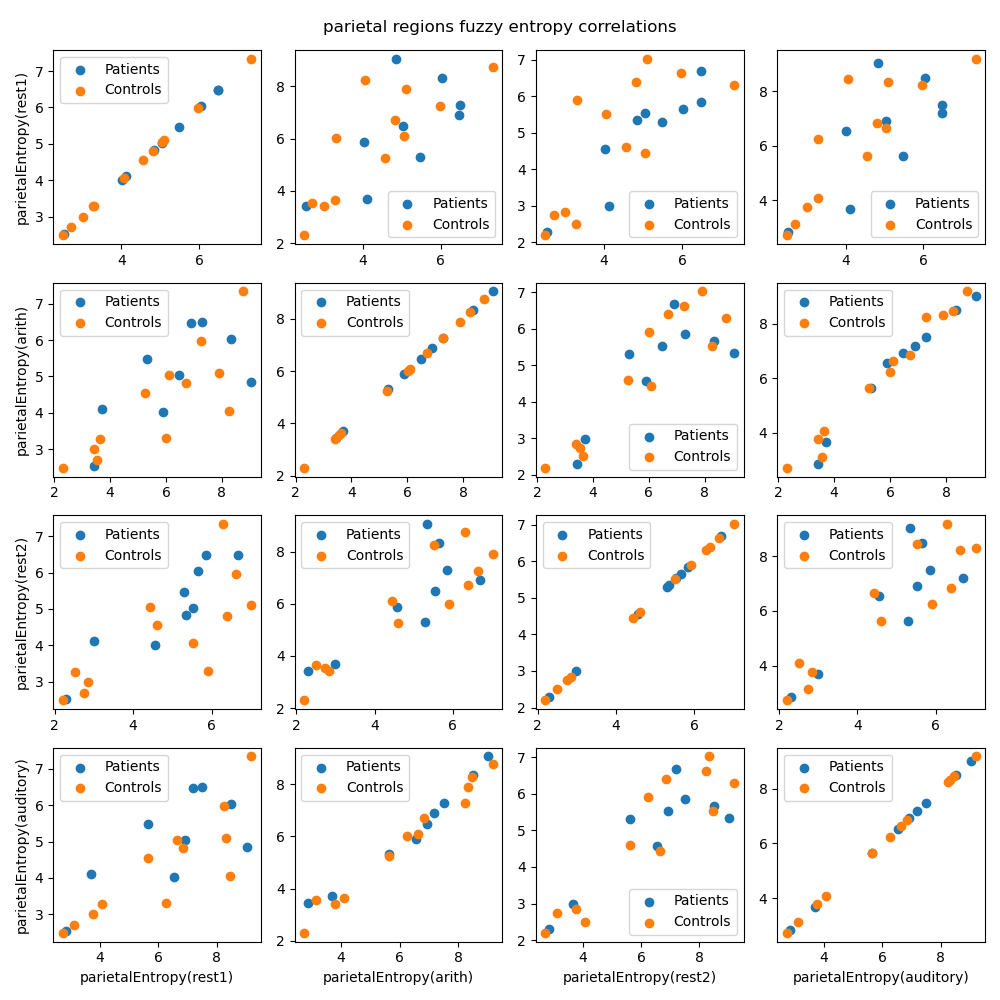
\includegraphics[width=16cm]{../../../data_analysis_results/FuzzEnt/parietal_region_corr.png}
  \caption{Parietal lobe Fuzzy-entropy}\label{parietal_fuzz}
\end{figure}
\begin{figure}[H]
  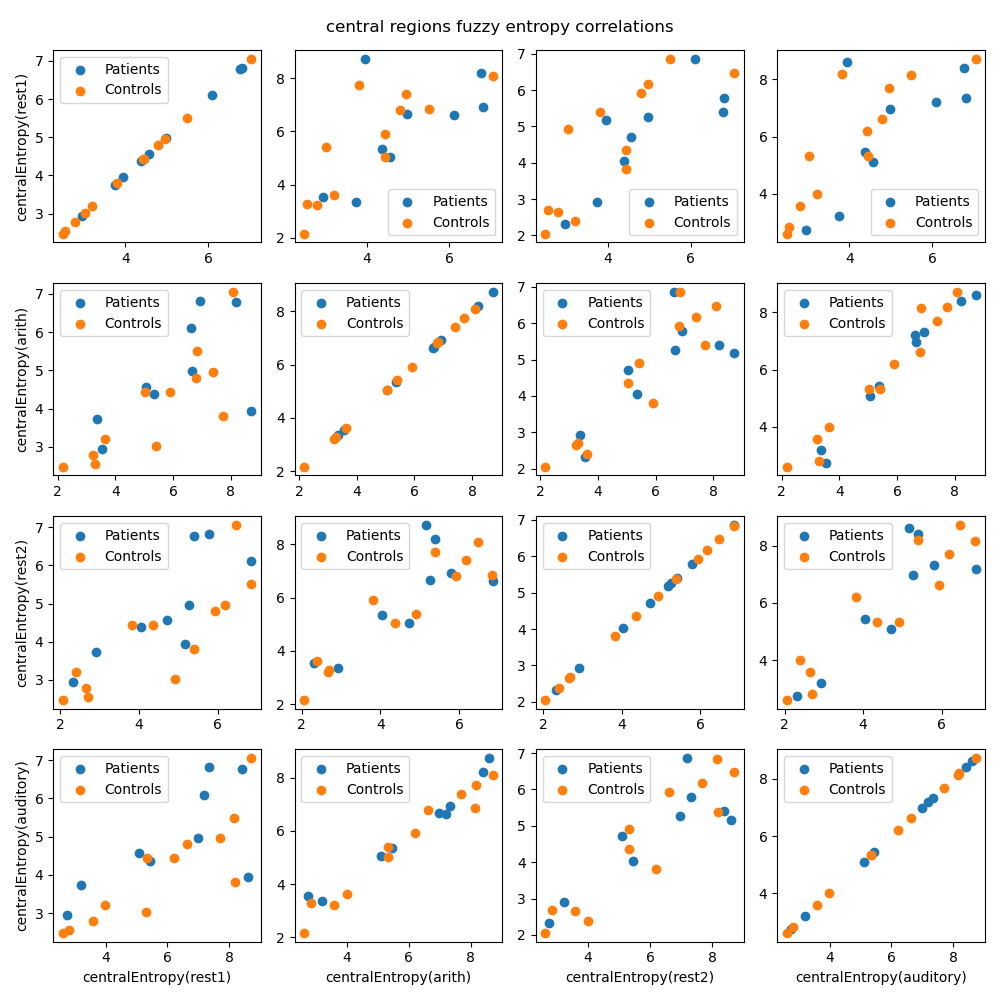
\includegraphics[width=16cm]{../../../data_analysis_results/FuzzEnt/central_region_corr.png}
  \caption{Central lobe Fuzzy-entropy}\label{central_fuzz}
\end{figure}
\begin{figure}[H]
  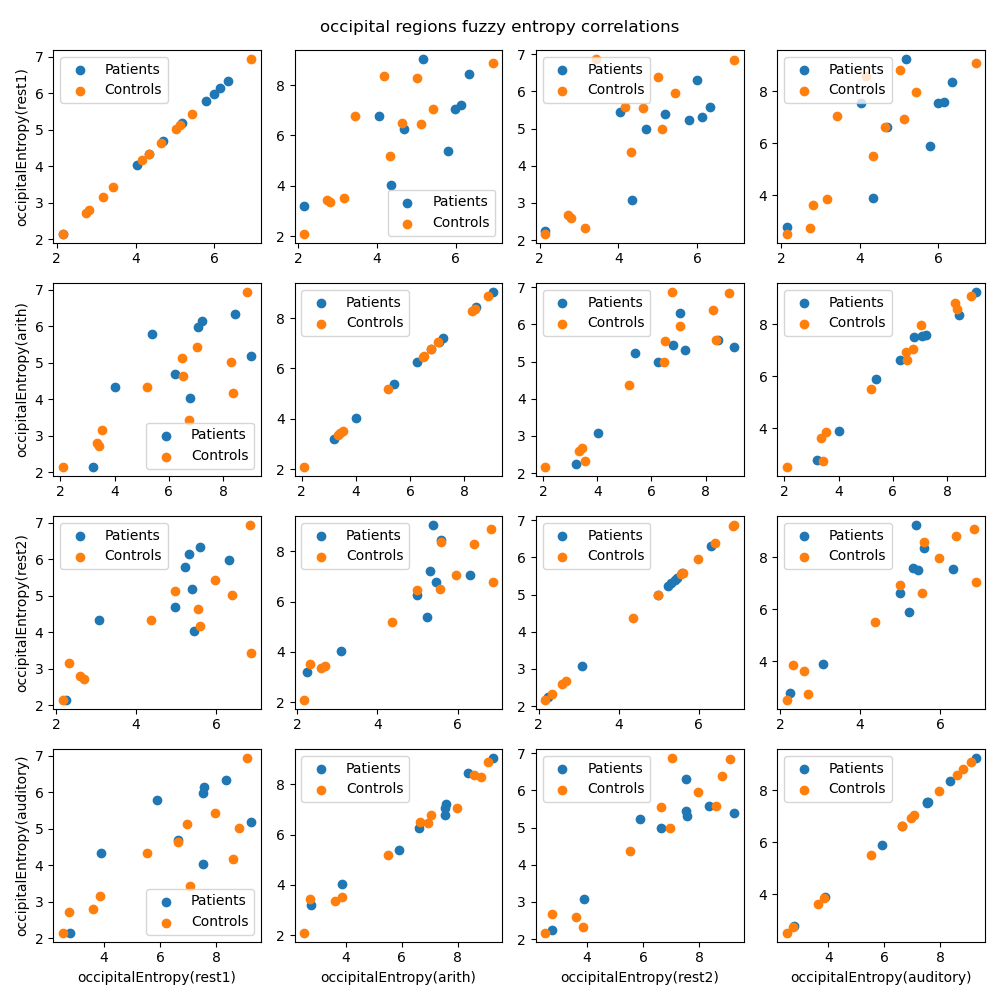
\includegraphics[width=16cm]{../../../data_analysis_results/FuzzEnt/occipital_region_corr.png}
  \caption{Occipital lobe Fuzzy-entropy}\label{occipital_fuzz}
\end{figure}
\begin{figure}[H]
  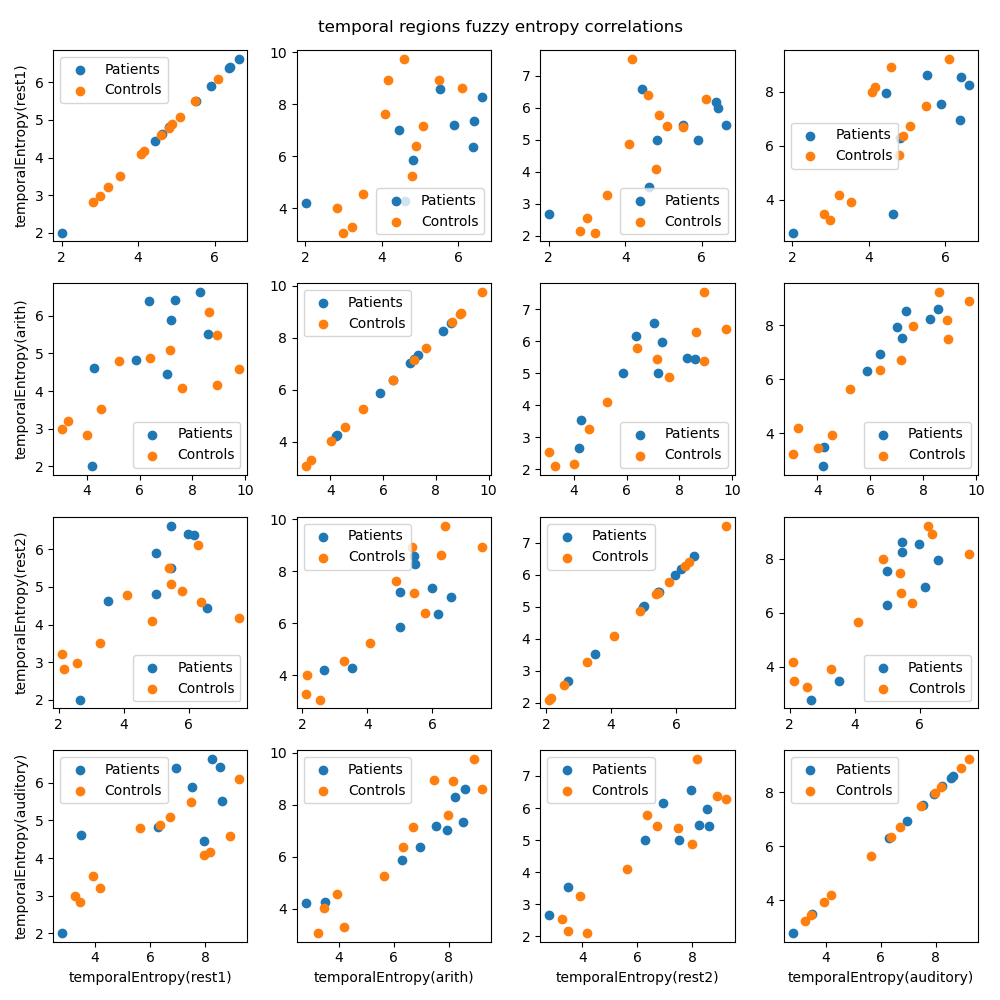
\includegraphics[width=16cm]{../../../data_analysis_results/FuzzEnt/temporal_region_corr.png}
  \caption{Temporal lobe Fuzzy-entropy}\label{temporal_fuzz}
\end{figure}

\end{document}
% \include{monthlly_report.acn}

%\journal{CSc 4110 Final Report}

%\title[journalExample]{Format for Project Reports}
\title{
  An update on the project: 
  \textbf{
      \textit{
        Development of an Automatic Instrument for Schizophrenia(SZ) Diagnosis
        }
      }, for the MCIP Innovation Prize 2022.
  }
% \author{
% Emmanuel OLATEJU \\
%     \begin{affiliation}
%       Supervised by Dr. K.P. Ayodele \\ 14/02/2023, \\
%       email: \mbox{kayodele@gmail.com, eoolateju@student.oauife.edu.ng}
%     \end{affiliation}
% }

\begin{document}
\maketitle

\section{Overview}
The purpose of this project is to design an instrument for early \gls{sz} diagnosis.
In designing the instrument, the following parts are to be developed:
\begin{itemize}
  \item An \gls{eeg} \gls{daq} system
  \item \gls{daq} user interface.
  \item Hand-clicker device for \gls{daq} process feedback from patient and clinicians.
  \item Machine/deep learning model.
  \item Soft instrument interacting with learnt model, \gls{daq} software, handheld 
  clicker, \gls{eeg} headbox and all developed parts.
  
\end{itemize}
The goal is to develop a medical turnkey device for \gls{sz} diagnosis having its own 
\gls{eeg} device and deeply embedded software. The long-term goal is for this turnkey device 
and its software to be built around the OpenBCI \gls{eeg} kit. The OpenBCI is chosen as
minimal number of electrode sites needed for \gls{sz} diagnosis may be identified and thus 
an \gls{eeg} kit that allows for flexibility of electrodes to be used is needed. This will 
mitigate the cost of the device making it more accessible. In the short term, the contec 
\gls{eeg} headbox is being used in identifying the best electrode sites.

The contec \gls{eeg} headbox is being used in place of the OpenBCI headbox temporarily 
for generation of the \gls{eeg} signals.
In order to fetch \gls{eeg} signals from the headbox, a piece of software that interacts 
with the contec's firmware has been developed. This piece of software has been incorporated 
with a user interface developed that makes \gls{daq} sessions interactive for both 
subjects and clinicians. The user interface and firmware interacting code together make 
up the Generis software presented in the first report.

In order to make \gls{daq} sessions more interactive, a handheld clicker is being developed 
to help patients and clinicians give feedback to the Generis software. Annotations can be 
somewhat a tough technical task and in certain cases becomes an headache for non-technical 
users. Once annotation messagess are configured into this clicker device, adding annotations 
will be redced to a task of simply clicking color coded buttons. This piece of hardware 
will also improve processing of signals as time during \gls{daq} of noise causing actions can be 
annotated and also times of subject inactivity or inert state to \gls{daq}. The handheld clicker 
is able to communicate with the Generis software through UART to USB communication.

In order to have an instrument of high accuracy and to solve the problem of \gls{sz} diagnosis 
being based on psychiatric nosology, the instrument(model) must be calibrated to seperate 
\glspl{szPtnt} from \glspl{hc}. This is being done using machine-learning and/or 
deep-learning methods and signal-processing algorithms to extract information relevant to 
\gls{sz} measurement and to improve discriminability.

The final instrument that integrates all of the designed parts is to be devloped upon 
completion of the handheld clicker and complete development of model to be used in 
measuring the extent of \gls{sz} disorder and classification of subjects. The structure 
of the final instrument is shown in the diagram below.
\begin{figure}[H]
  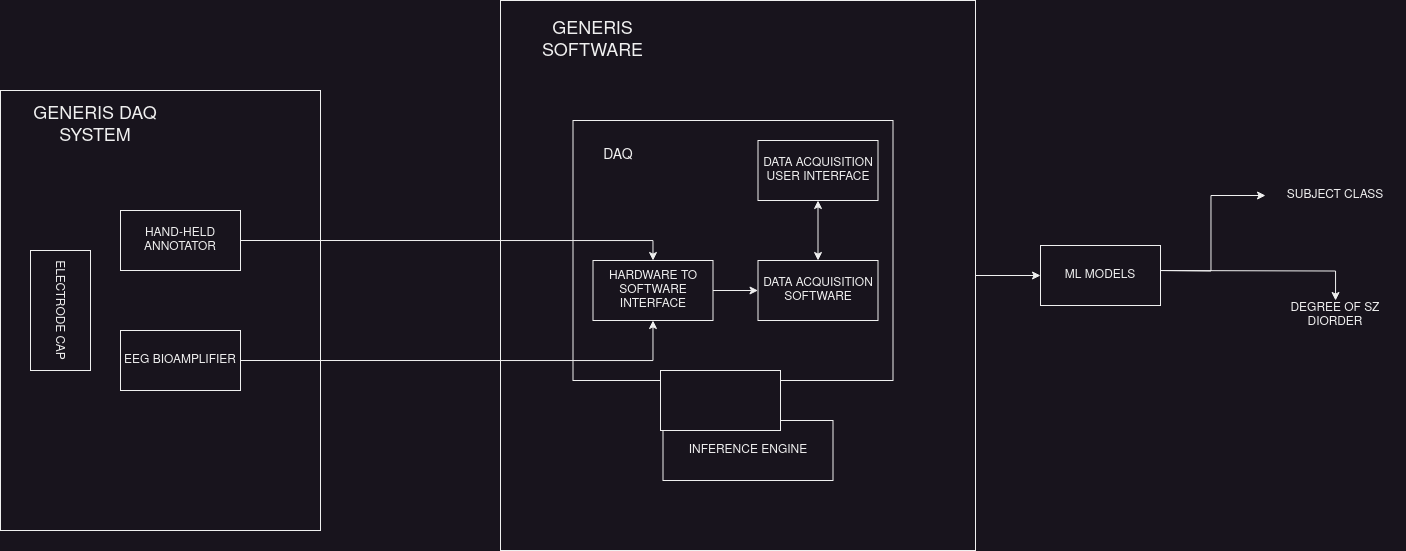
\includegraphics[width=16cm]{../../../images/technical/instrument.drawio.png}
  \caption{\gls{sz} diagnosis instrument}\label{instrument}
\end{figure}


\section{Handheld clicker}
The handheld clicker design is based on an arduino nano which applies the output of four 
tact switches as inputs to four vectored interrupts on the nano development board. The 
exact labels of these inputs has not been assigned as a study of the erogonomics of 
conventions employed in other devices of this kind and how best conventions are adapted and 
modified for the use case of this project is being studied. 

The current design of the handheld clicker(annotator) is the second iteration and is referred 
to as HC-v0.2. 
The circuit diagram of the handheld clicker is given in figure \ref{clicker_circuit}.
The flowchart describing the algorithm of this device is shown in figure \ref{clicker_flowchart}. 
The front and top images of the hand-clicker-v0.2 are shown in figures \ref{clicker} and 
\ref{top_view_of_clicker}.
\begin{figure}[H]
  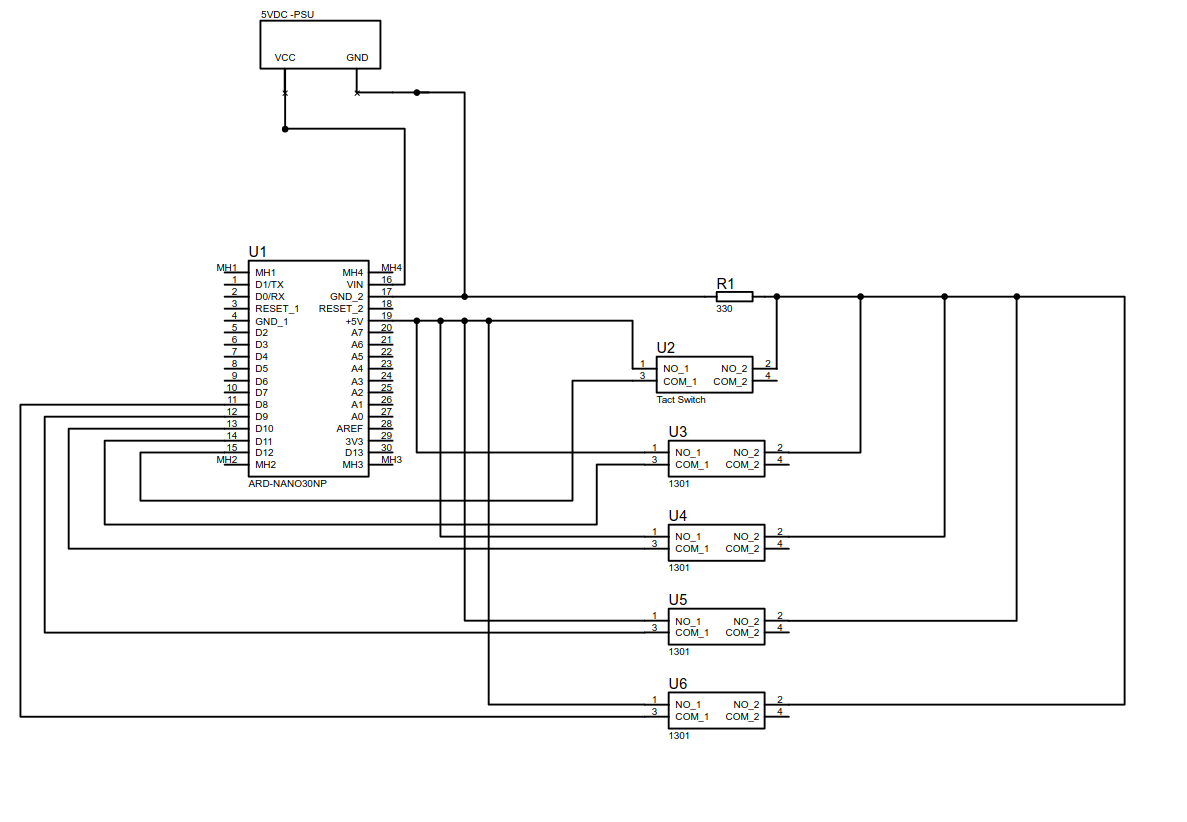
\includegraphics[width=16cm]{../../../hardware/handheld_clicker/circuit_image.png}
  \caption{handheld clicker circuit}\label{clicker_circuit}
\end{figure}
\begin{figure}[H]
  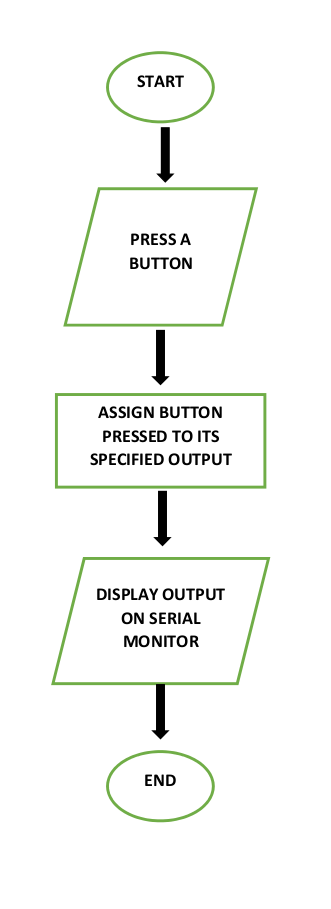
\includegraphics[height=16cm,width=10cm]{../../../hardware/handheld_clicker/flowchart.png}
  \caption{Flowchart algorithm of clicker}\label{clicker_flowchart}
\end{figure}
\begin{figure}[H]
  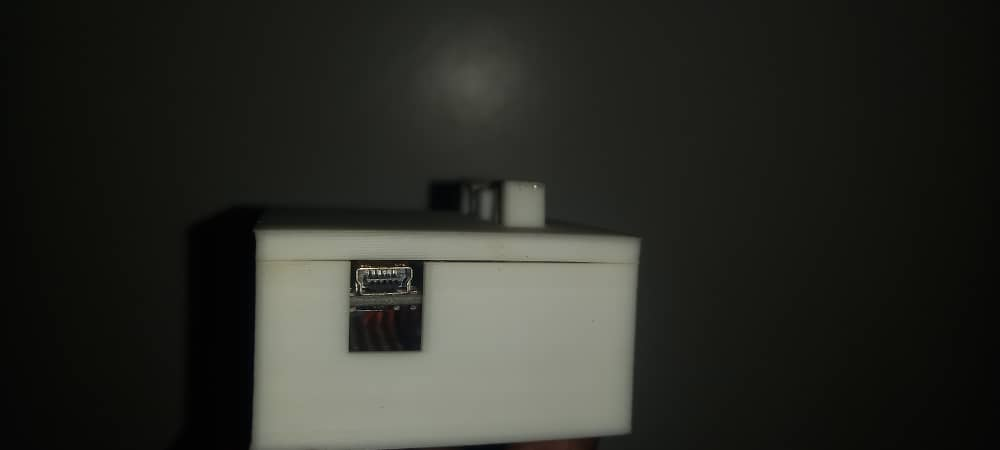
\includegraphics[width=16cm]{../../../hardware/handheld_clicker/front.jpeg}
  \caption{Front view of clicker}\label{clicker}
\end{figure}
\begin{figure}[H]
  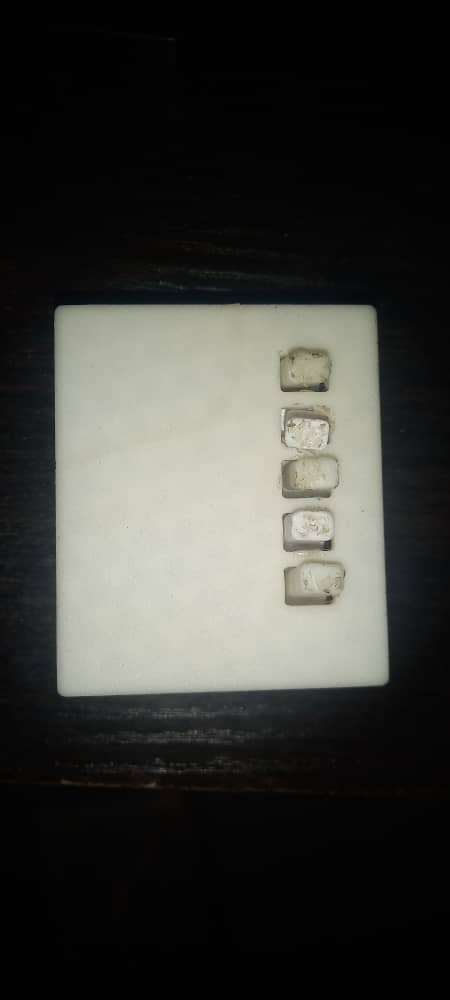
\includegraphics[,height=10cm,width=8cm]{../../../hardware/handheld_clicker/top.jpeg}
  \caption{Top view of clicker}\label{top_view_of_clicker}
\end{figure}


\section{Model Development (Feature-extraction, Data-analysis)}
\subsection{Feature Extraction}
March's report presented the fuzzy entropy features extracted from cortical
regions during phases of \gls{daq} and also the refined \gls{mmn} plots which 
made the \gls{mmn} waveform more evident. Relevant changes made to features 
extraction highlighted in marchs's report includes:
\begin{itemize}
  \item Recomputing the \gls{mmn} waveforms
  \item Spatial dimension augmentation with gaussian noise during computation of fuzzy-entropy
  \item Development of custom fuzzy-entropy library
\end{itemize}
The following was proposed as the next set of action points:
\begin{itemize}
  \item The continued improvement of fuzzy-entropy library to work with multivariate \\
  time-series(2D data)
  \item comparing performance of the fuzzy-entropy features from sourced library to \\
  that of the personally developed library
  \item Computing the auditory steady state features
\end{itemize}
A slight detour was made from these proposed action points for the month of april. 
Analysis of the extracted features for levels of dicriminability was carried out 
to understand how to improve the features extraction methods. The analysis shows 
a significant level of discrimination in the \gls{mmn} features, less in the 
fuzzy-entropy features, though the correlation patterns of the fuzzy-entropy features 
suggest they might carry information on extent of \gls{sz} disorder.

\gls{mmn} features have been extracted from the scaled \gls{mmn} waveforms. The 
\gls{mmn} features were computed as the mean of the \gls{mmn} waveforms within 
the time-frames 0-100ms, 100-200ms, 200-300ms, 300-400ms, 400-450ms.

Formerly implemented montage plot algorithm was improved upon to reduce 
time-complexity so as to make data visualization and analysis easier to obtain 
intuitive information from.

\subsection{Data Analysis/Visualization}\label{data_analyis}
 Analysis of the extracted features was done to establish the quality of discriminative 
 and quantitative information contained in the extracted features. The method of 
 Visualization of some of these features changed to make analysis easy.
 The results of the analysis are given in section \ref{figures}. Visualization methods 
 and analysis carried out includes:
\begin{itemize}
  \item Comparing \gls{mmn} feature values for 1KHz duration deviant and 3KHz frequency deviant 
  between patient and controls across all electrodes and time windows.
  (Figures \ref{mmnvalue_0_100ms} - \ref{mmnvalue_400_450ms})
  \item Converting the \gls{mmn} values to montage plots for 1KHz duration deviant 
  and 3KHz frequency deviant for easier interpretation and analyzing montage evolution.
  (Figures \ref{control_1KHz_mmn_montage}-\ref{patient_3KHz_mmn_montage})
  \item Comparing distribution of computed fuzzy-entropy values of patients and controls 
  for each cortical region across all phases of \gls{daq}.
  (Figures \ref{fig:controlFuzzEnt}-\ref{fuzz_ent_distributions}) 
  \item Correlating fuzzy-entropy values from cortical regions across 
  all phases of \gls{daq}.(Figure \ref{fuzz_ent_corr_mat})
  \item Comparing entropies from all cortical regions for each phase of \gls{daq}.
  (Figures \ref{rest_fuzz}-\ref{auditory_fuzz})
  \item Comparing entropies from all phases of \gls{daq} for each cortical region.
  (figures \ref{frontal_fuzz}-\ref{temporal_fuzz})
\end{itemize} 

\section{Inference and Action Points}
\subsection{Inference}
From the analysis carried out, the \gls{mmn} features of both tone deviants show 
discriminative properties between the \gls{szPtnt} and \gls{hc} in localized head 
regions. The fuzzy-entropy features do not show discriminative abilities, but their 
correlation patterns indicate a linear relationship that might be a measure of degree 
of \gls{sz} disorder. Therefore we need to find methods that improve quality of extracted 
features and proceed with developing a learner model.

\subsection{Action Points}
Based on the inference drawn, the action points for the month of may is as follows:
\begin{itemize}
  \item Computing the auditory steady state features.
  \item Re-computing fuzzy-entropy features using other libraries and 
  comparing performance.
  \item Improve discriminability of features using spatial filters and dimensionality 
  reduction techniques.
  \item Compare performance of a custom mutilayer feedforward network and traditional 
  machine-learning algorithms for classification and estimation of measures of degree 
  of \gls{sz} disorder.
\end{itemize}

\section{Figures}\label{figures}

\begin{figure}[H]
  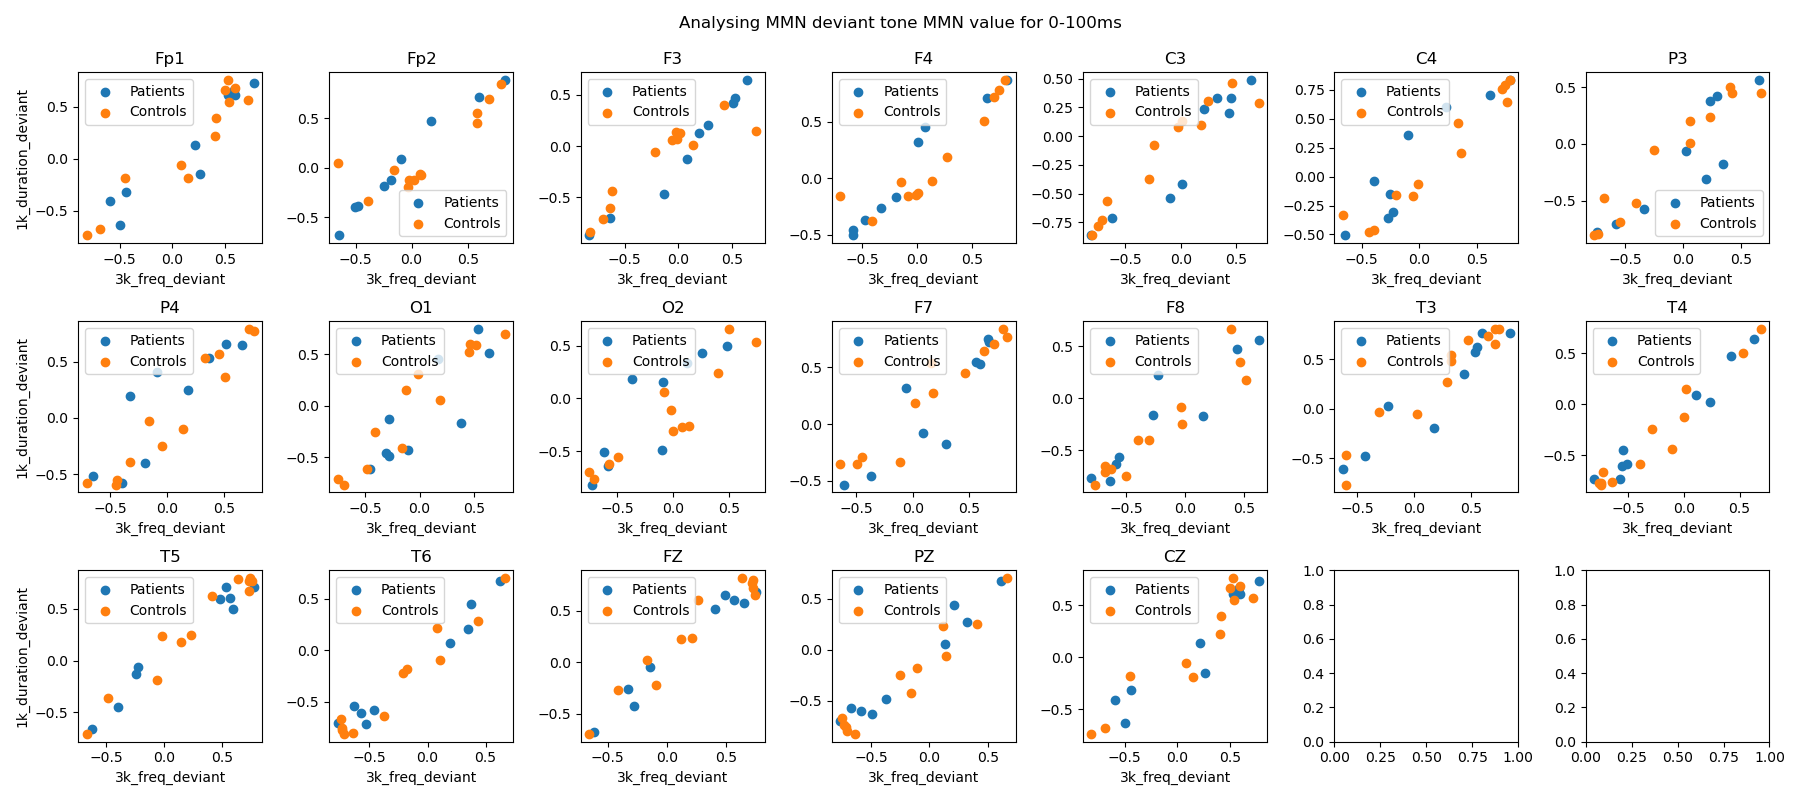
\includegraphics[width=16cm]{../../../data_analysis_results/MMN/features/deviant_tone_0.png}
  \caption{\gls{mmn} values from 0-100ms}\label{mmnvalue_0_100ms}
\end{figure}
\begin{figure}[H]
  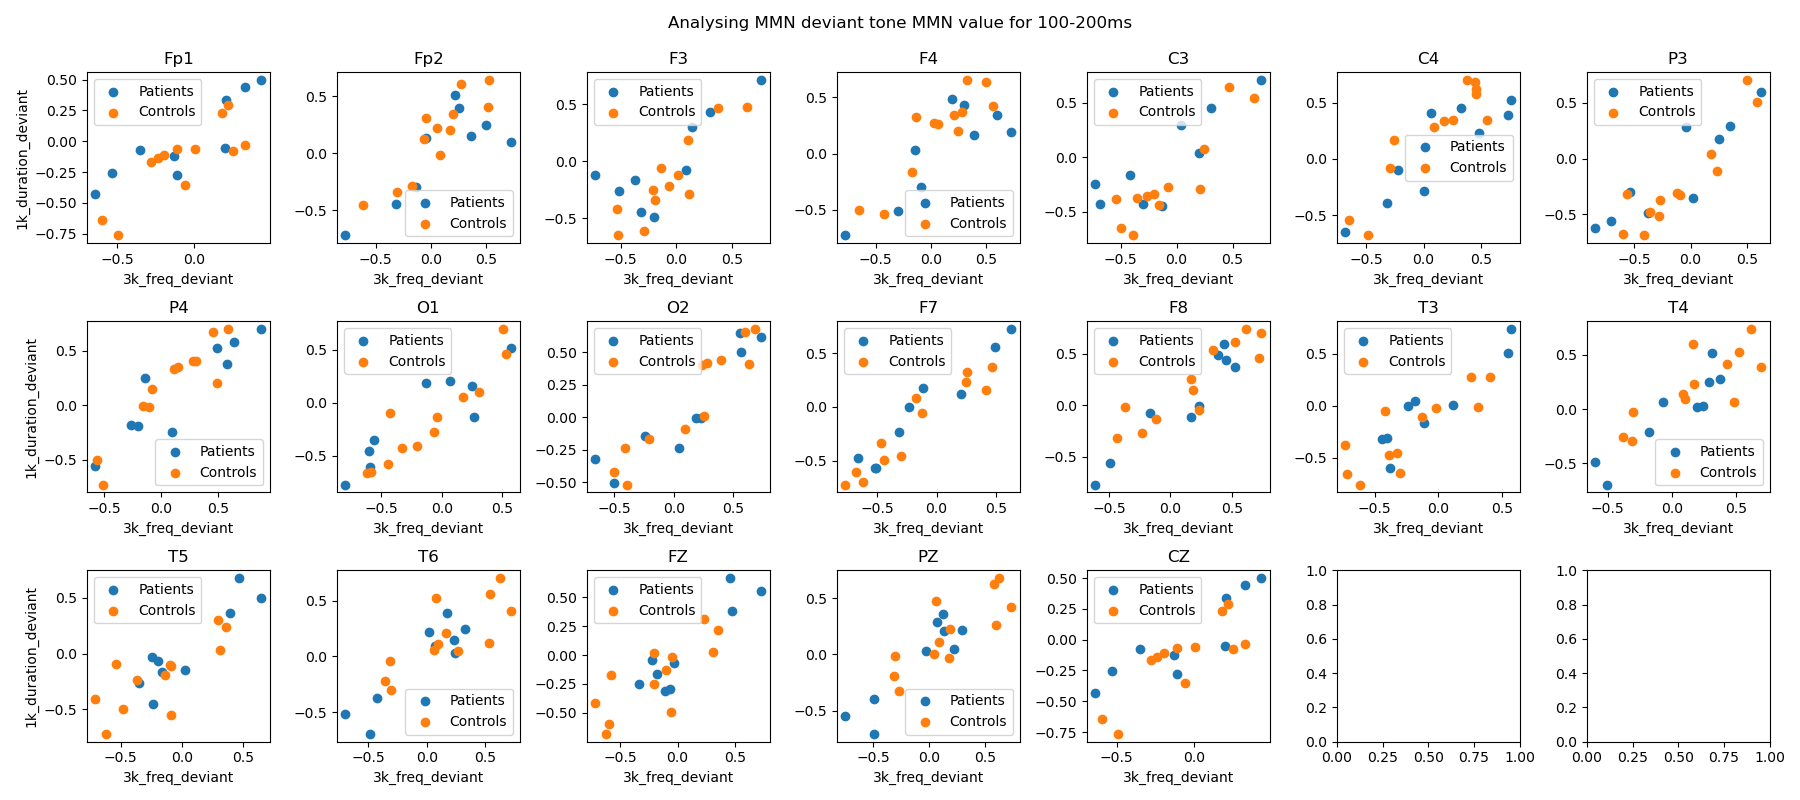
\includegraphics[width=16cm]{../../../data_analysis_results/MMN/features/deviant_tone_1.png}
  \caption{\gls{mmn} values from 100-200ms}\label{mmnvalue_100_200ms}
\end{figure}
\begin{figure}[H]
  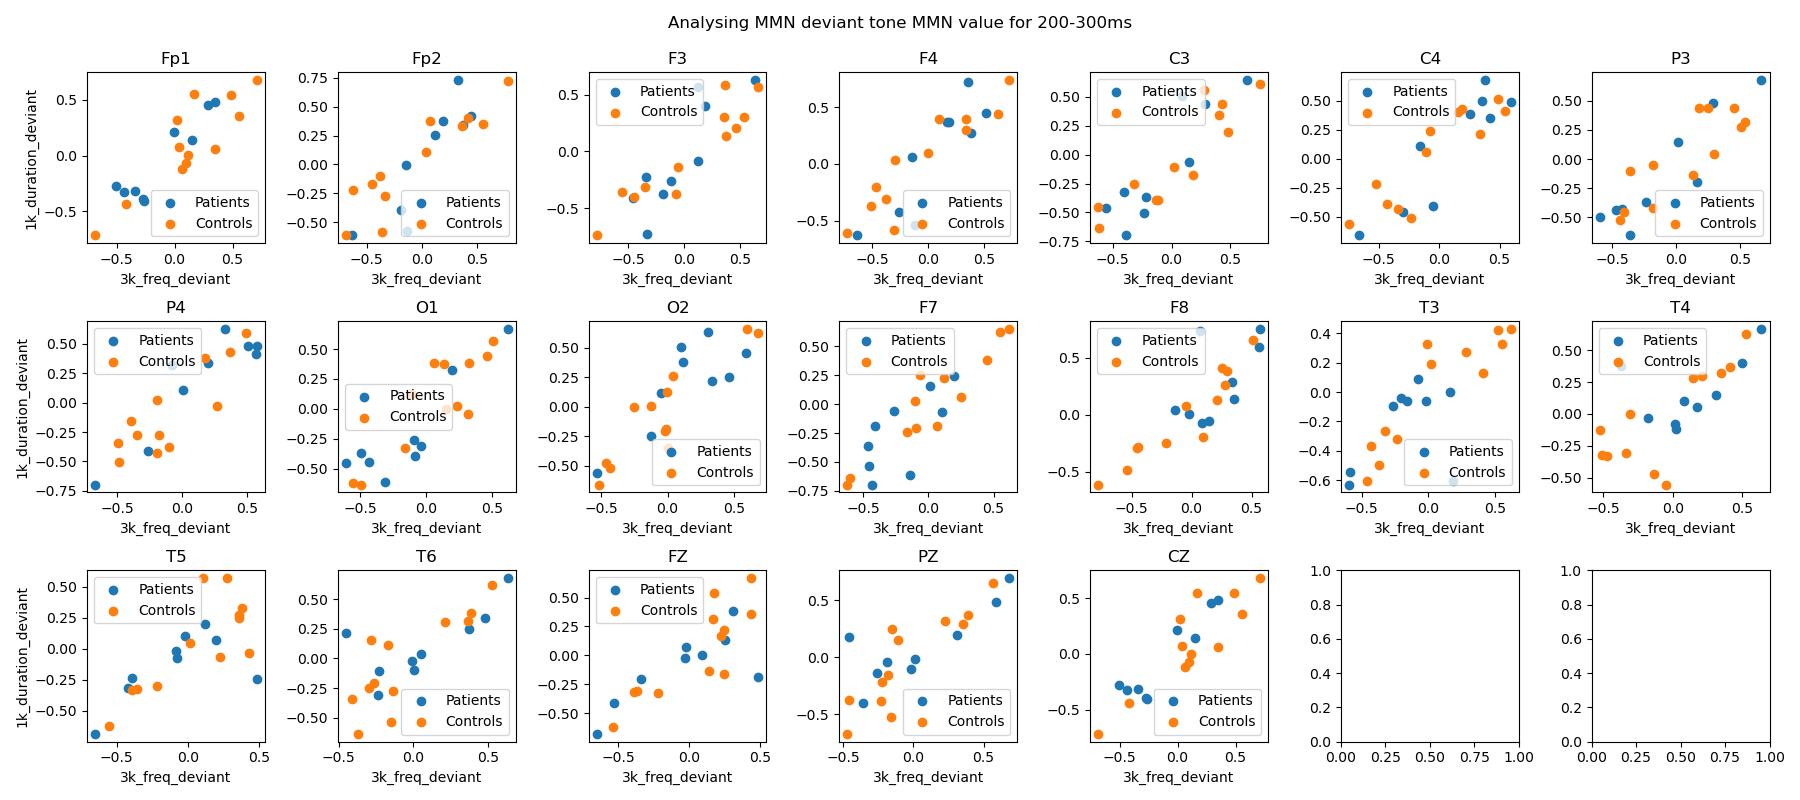
\includegraphics[width=16cm]{../../../data_analysis_results/MMN/features/deviant_tone_2.png}
  \caption{\gls{mmn} values from 200-300ms}\label{mmnvalue_200_300ms}
\end{figure}
\begin{figure}[H]
  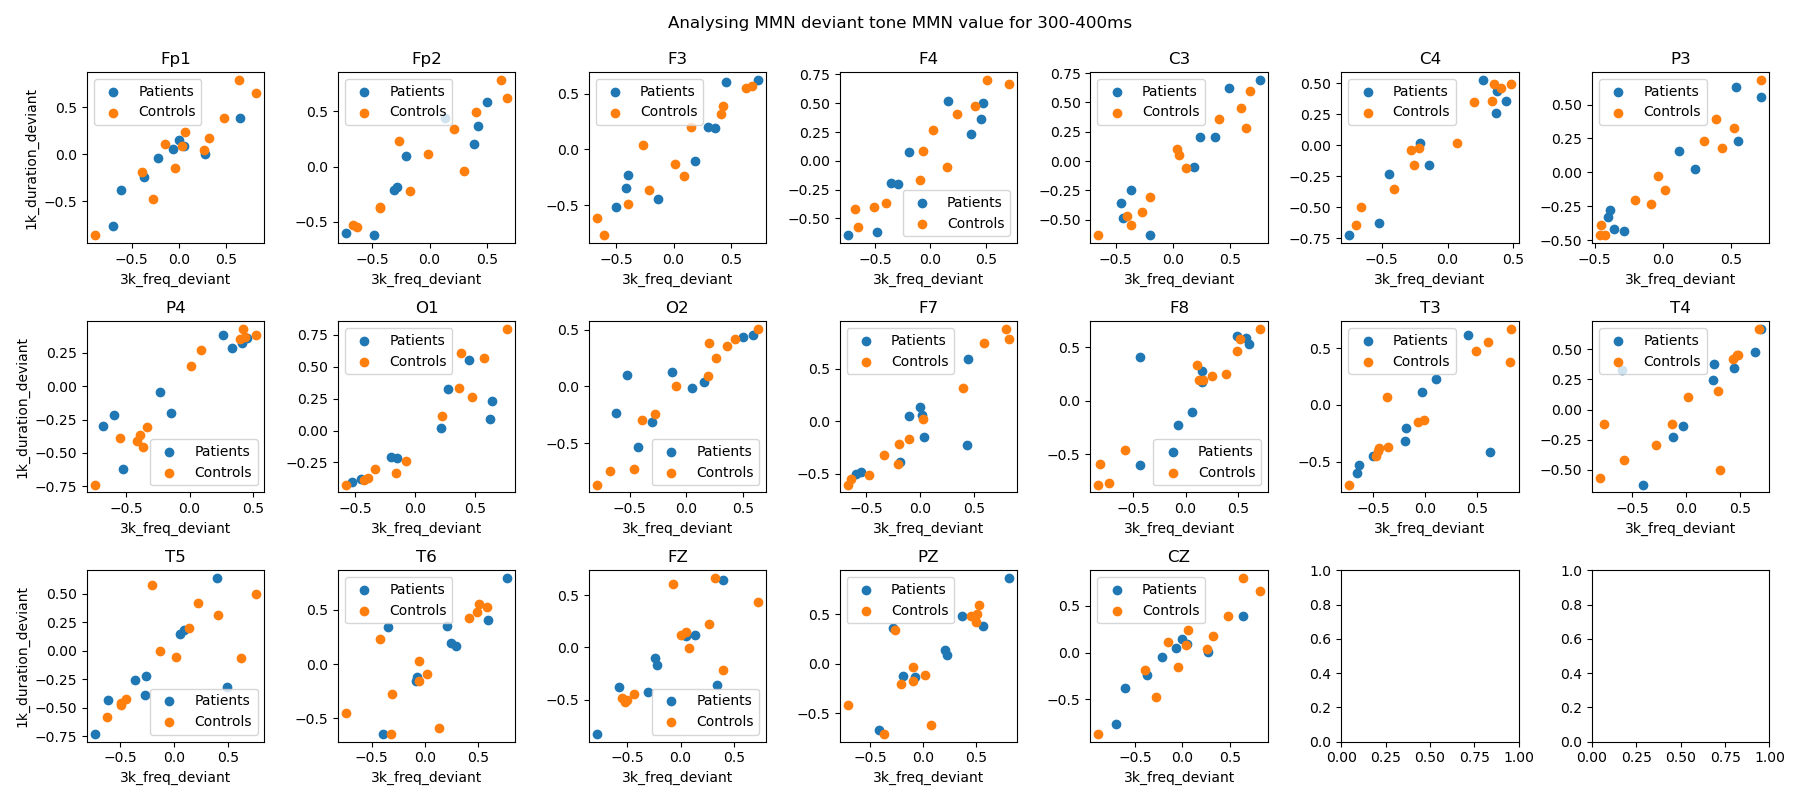
\includegraphics[width=16cm]{../../../data_analysis_results/MMN/features/deviant_tone_3.png}
  \caption{\gls{mmn} values from 300-400ms}\label{mmnvalue_300_400ms}
\end{figure}
\begin{figure}[H]
  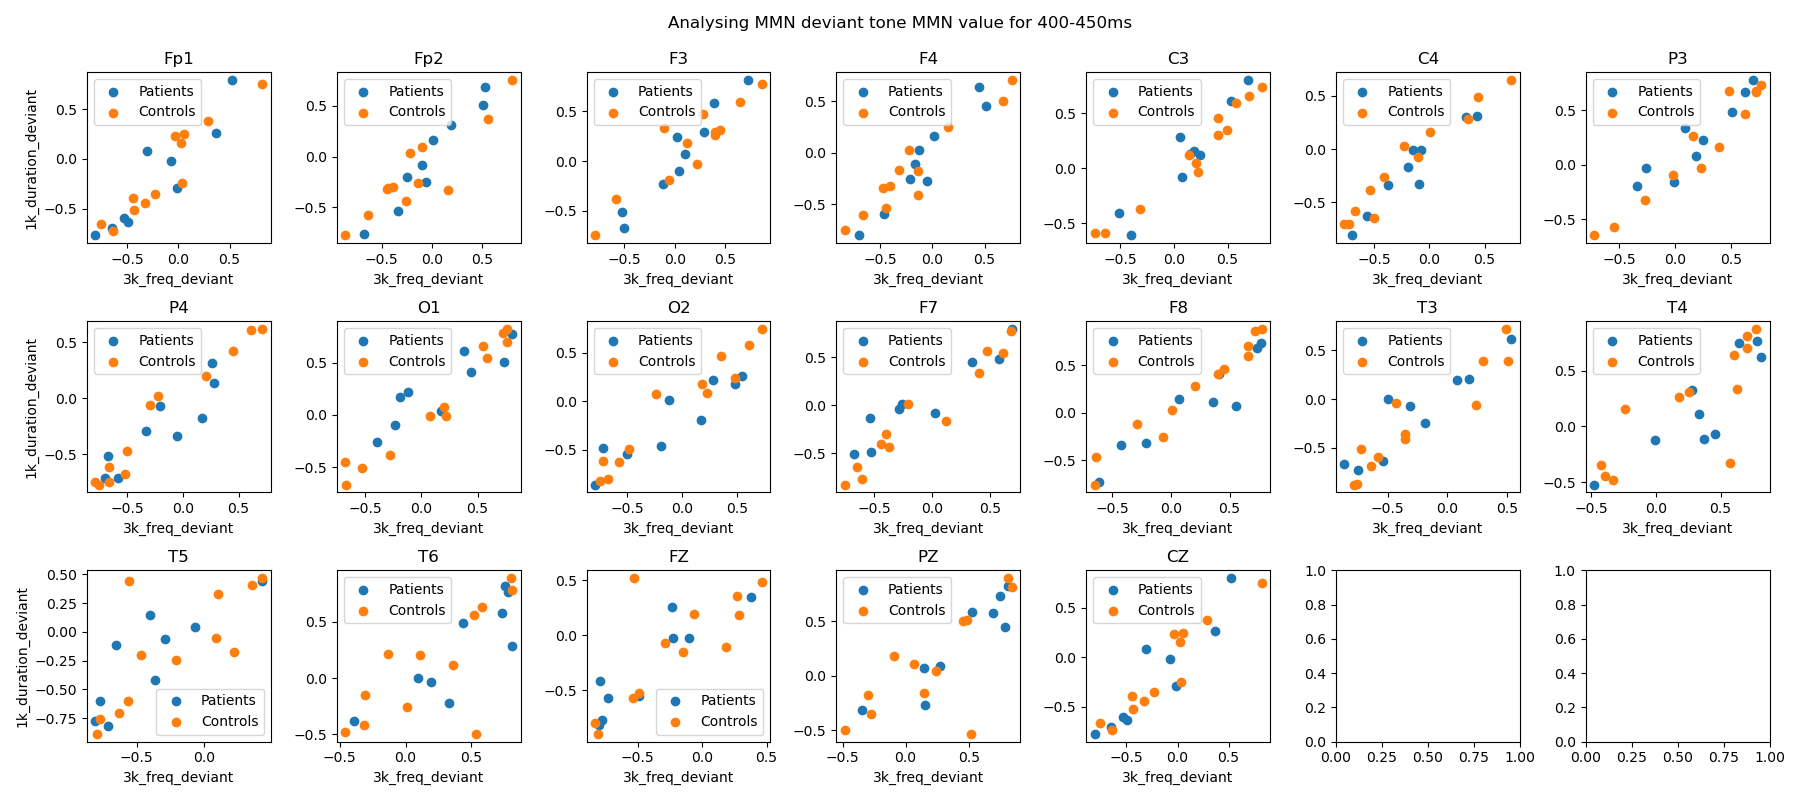
\includegraphics[width=16cm]{../../../data_analysis_results/MMN/features/deviant_tone_4.png}
  \caption{\gls{mmn} values from 400-450ms}\label{mmnvalue_400_450ms}
\end{figure}

\begin{figure}[H]
  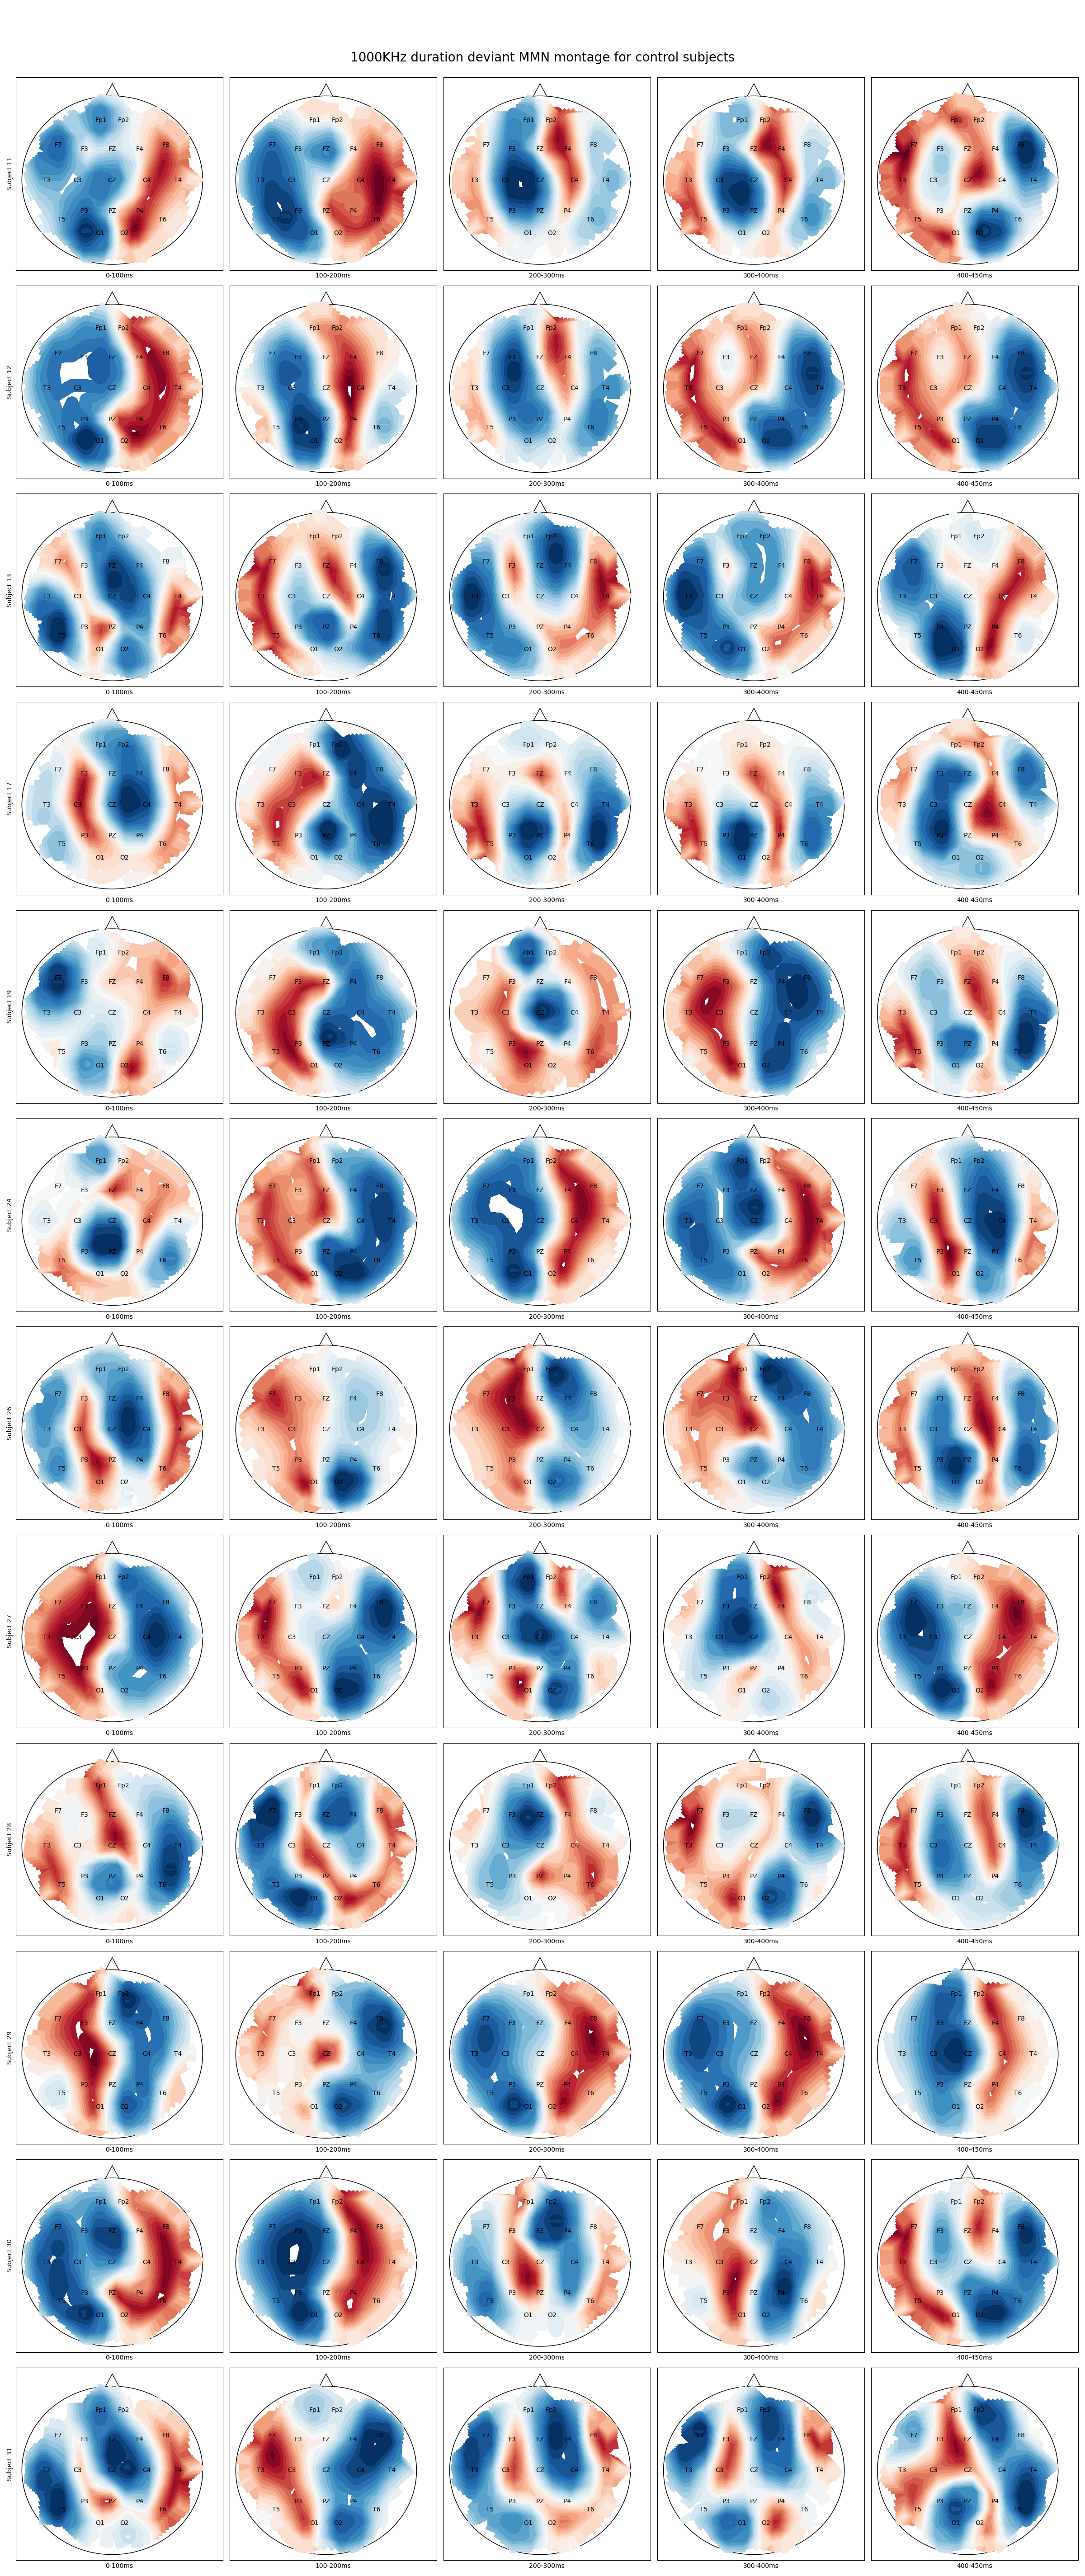
\includegraphics[width=16cm]{../../../data_analysis_results/MMN/montage/Control/1KHz_duration_deviant_montage.png}
  \caption{Controls 1KHz duration deviant \gls{mmn} value montage}\label{control_1KHz_mmn_montage}
\end{figure}
\begin{figure}[H]
  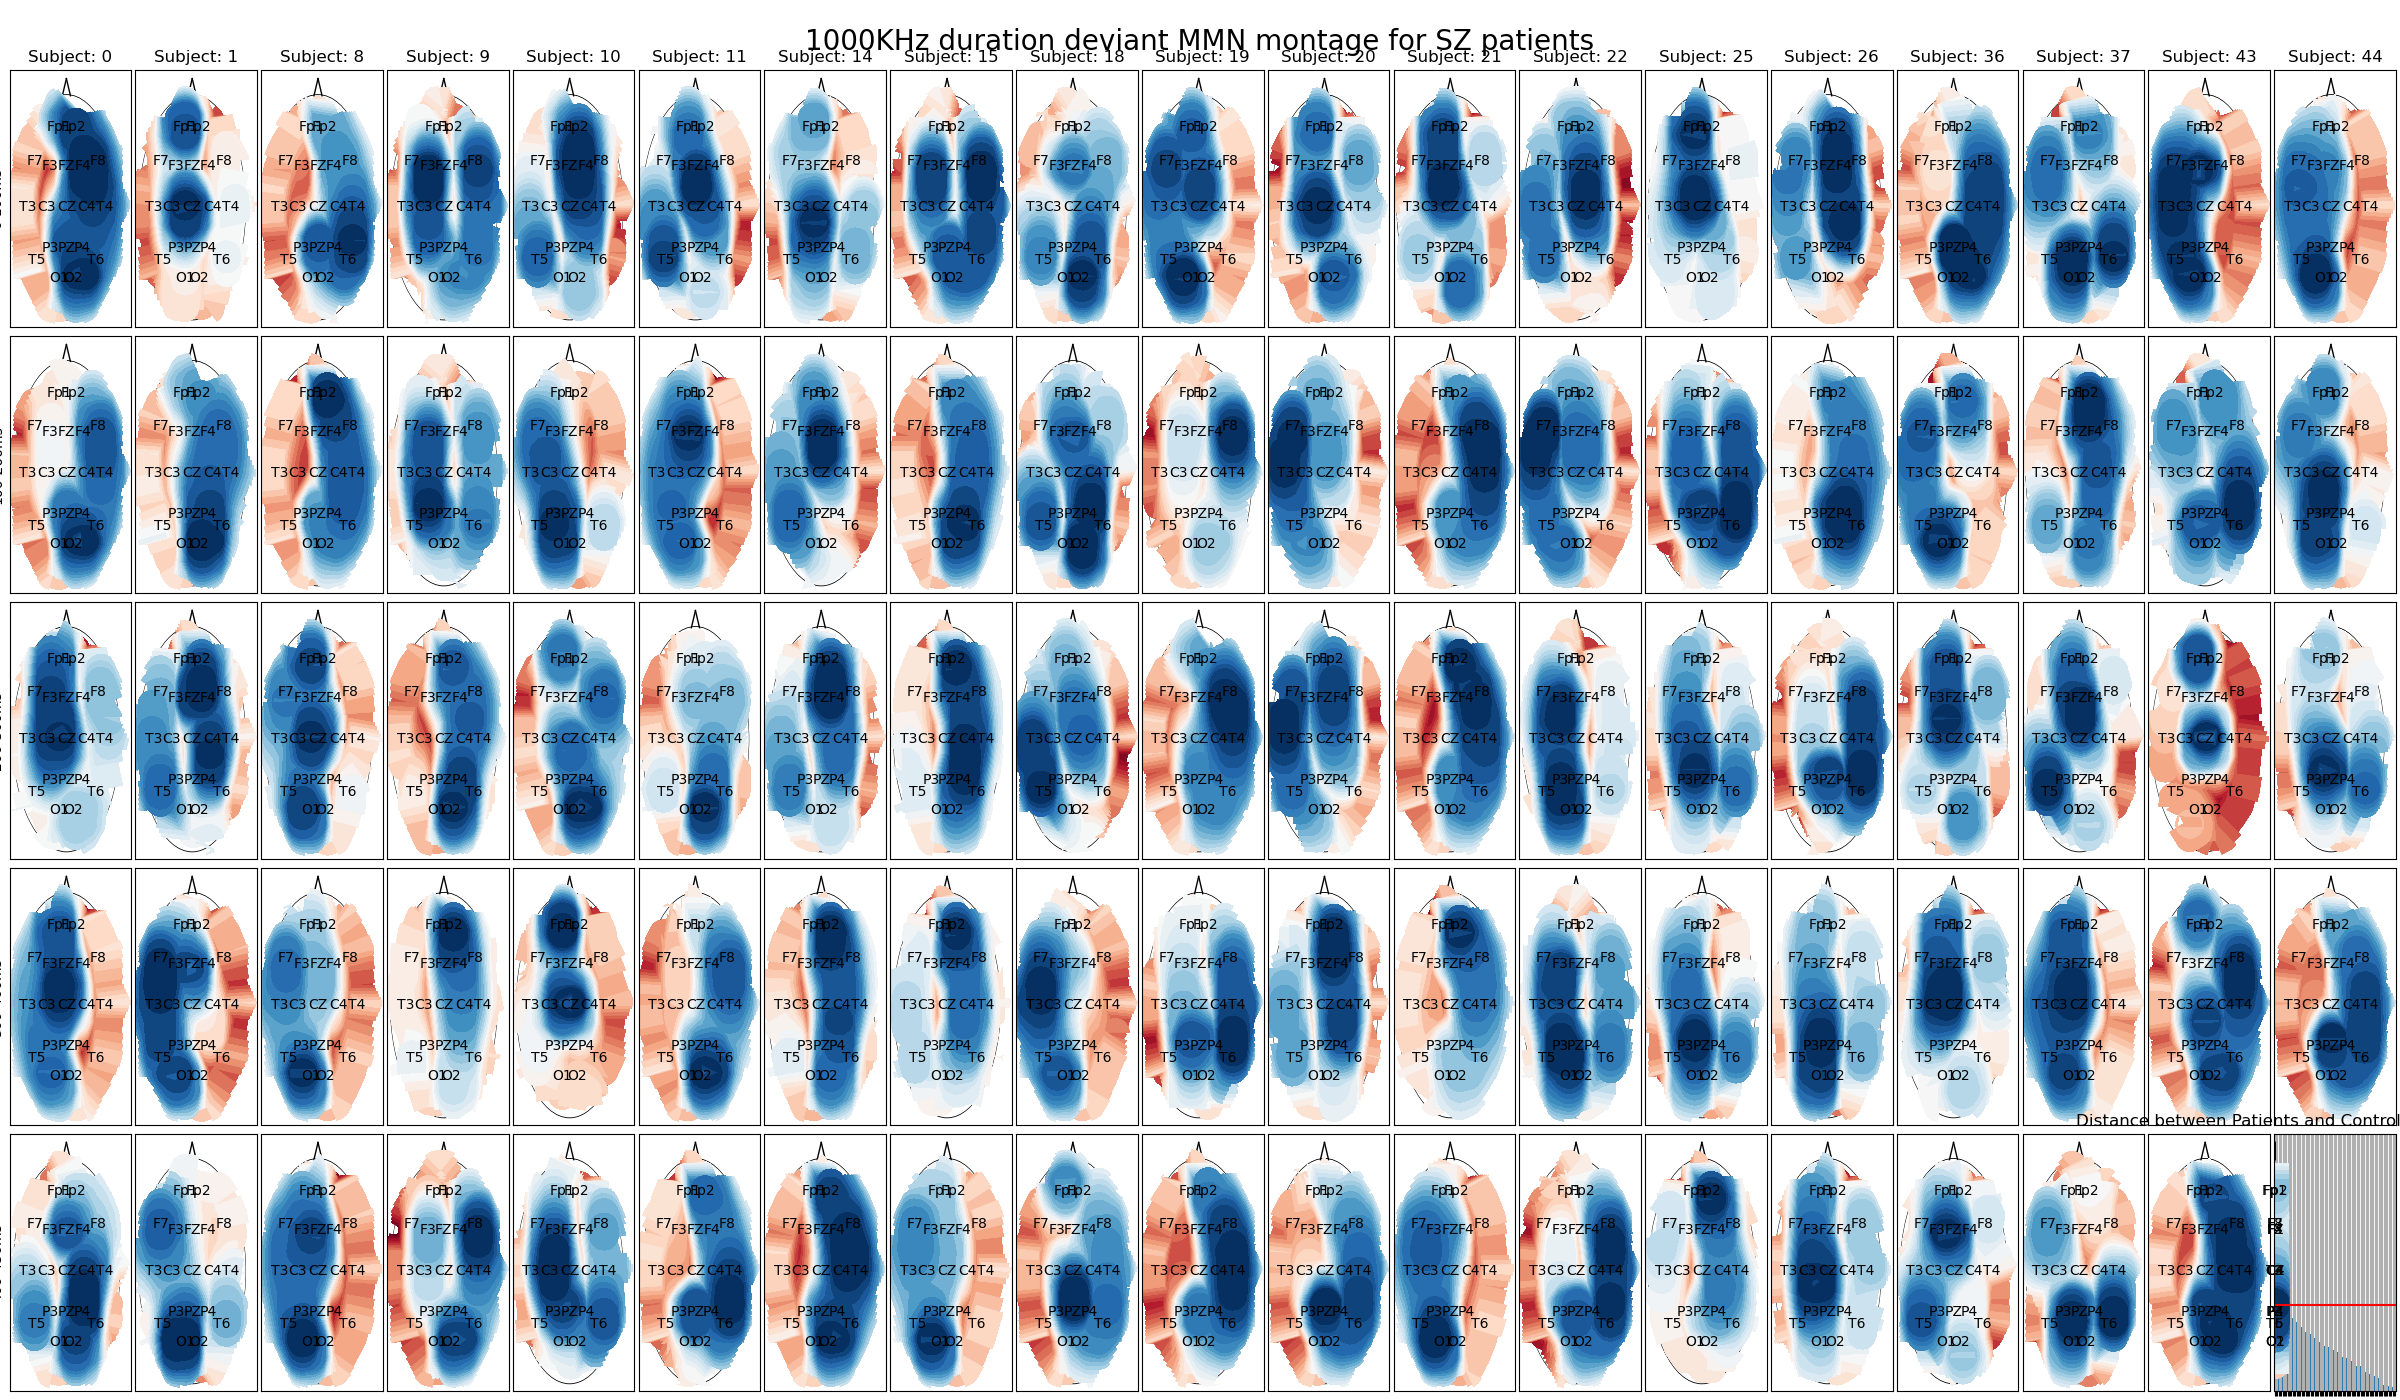
\includegraphics[width=16cm]{../../../data_analysis_results/MMN/montage/Patient/1KHz_duration_deviant_montage.png}
  \caption{Patients 1KHz duration deviant \gls{mmn} value montage}\label{patient_1KHz_mmn_montage}
\end{figure}
\begin{figure}[H]
  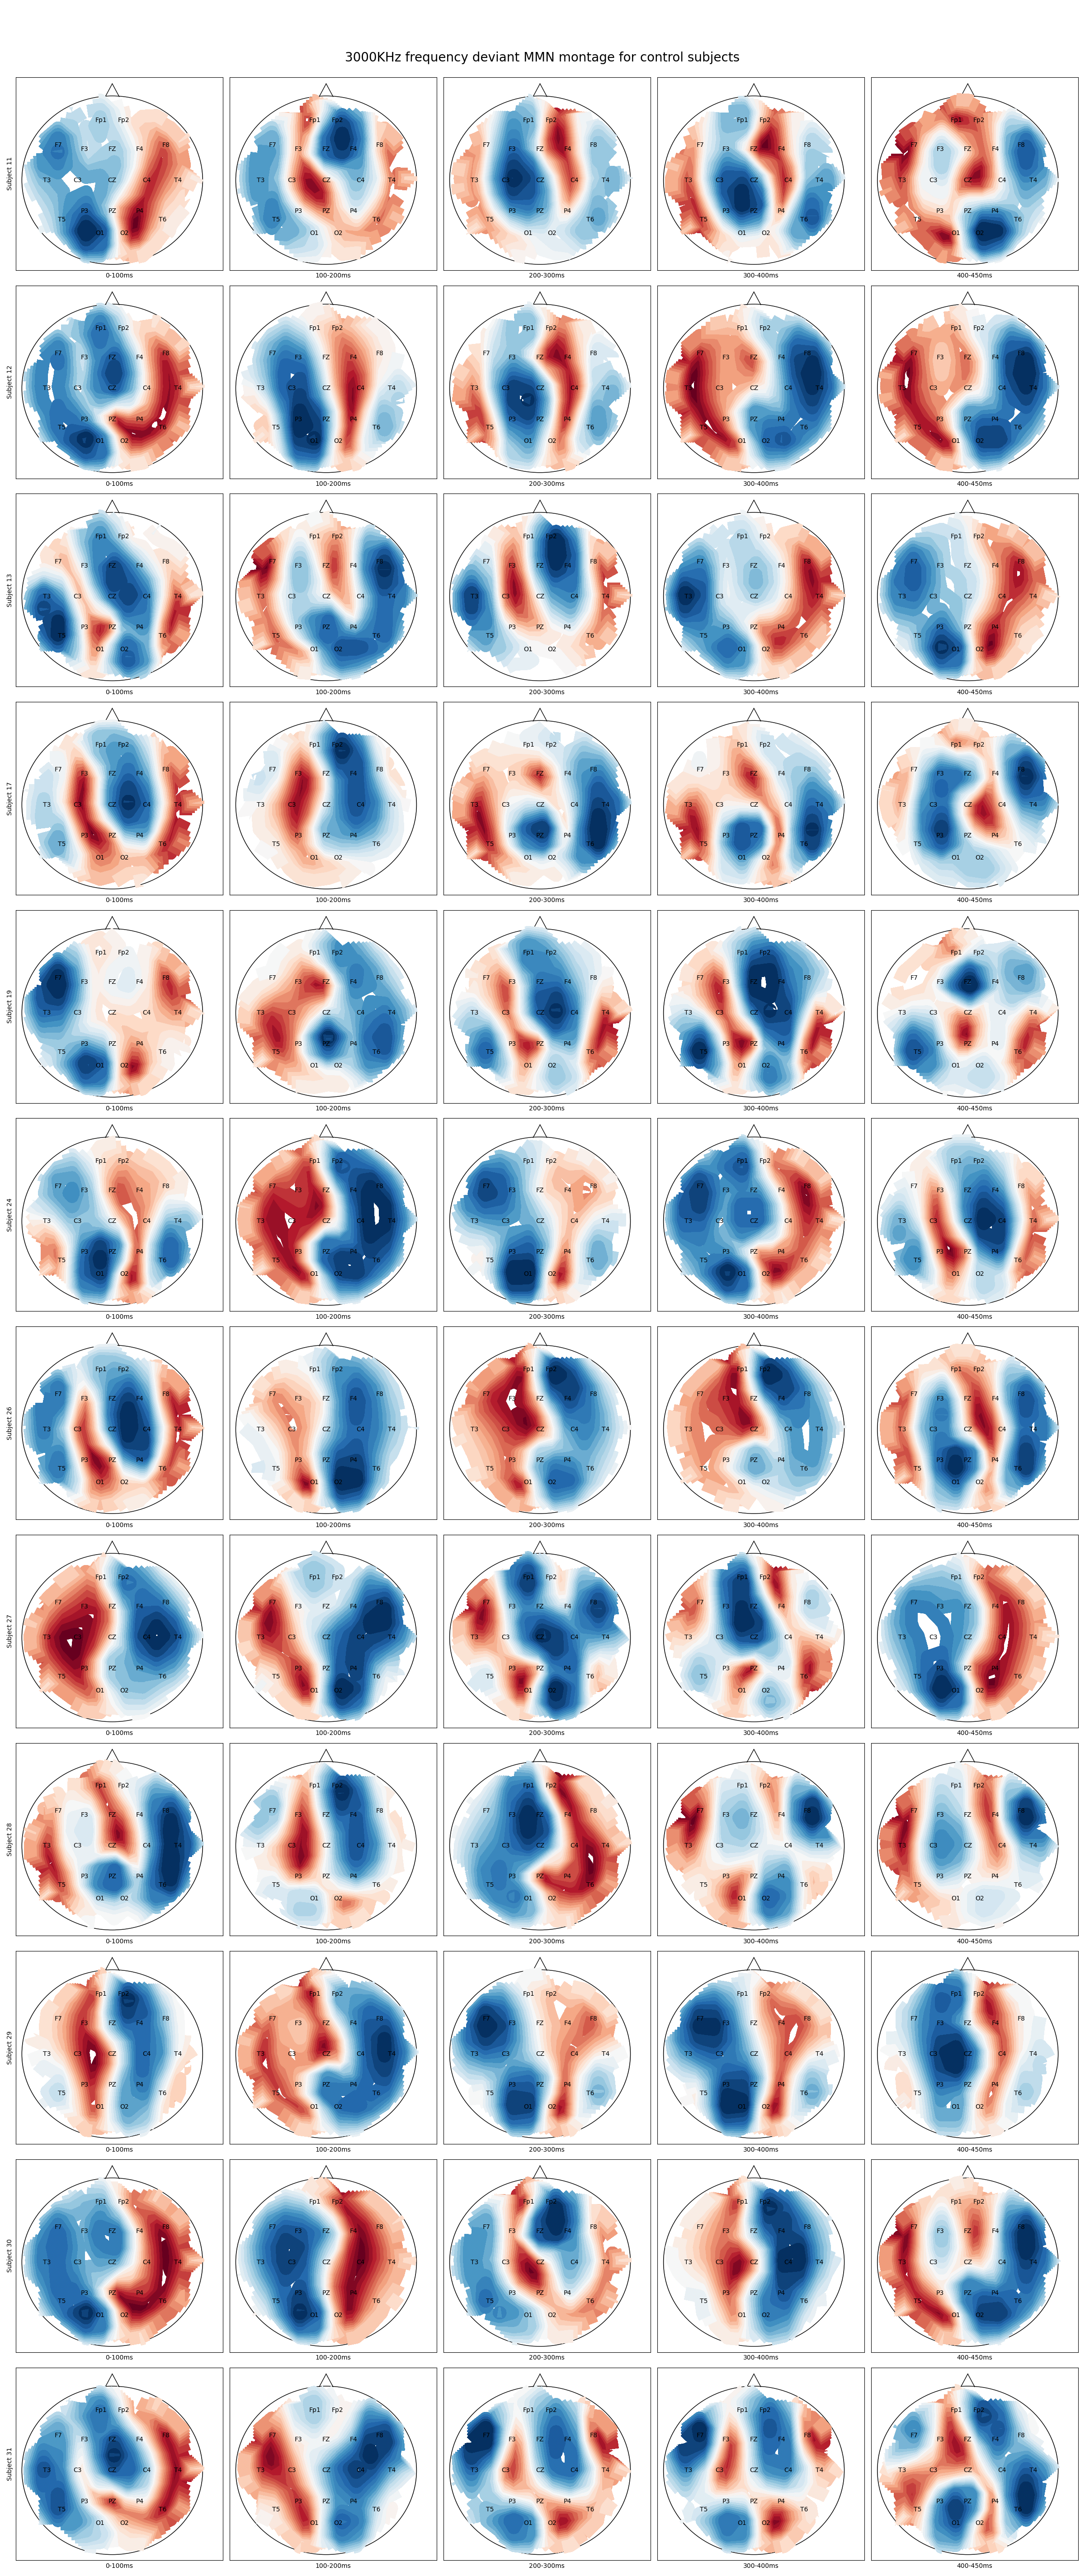
\includegraphics[width=16cm]{../../../data_analysis_results/MMN/montage/Control/3KHz_frequency_deviant_montage.png}
  \caption{Controls 3KHz frequency deviant \gls{mmn} value montage}\label{control_3KHz_mmn_montage}
\end{figure}
\begin{figure}[H]
  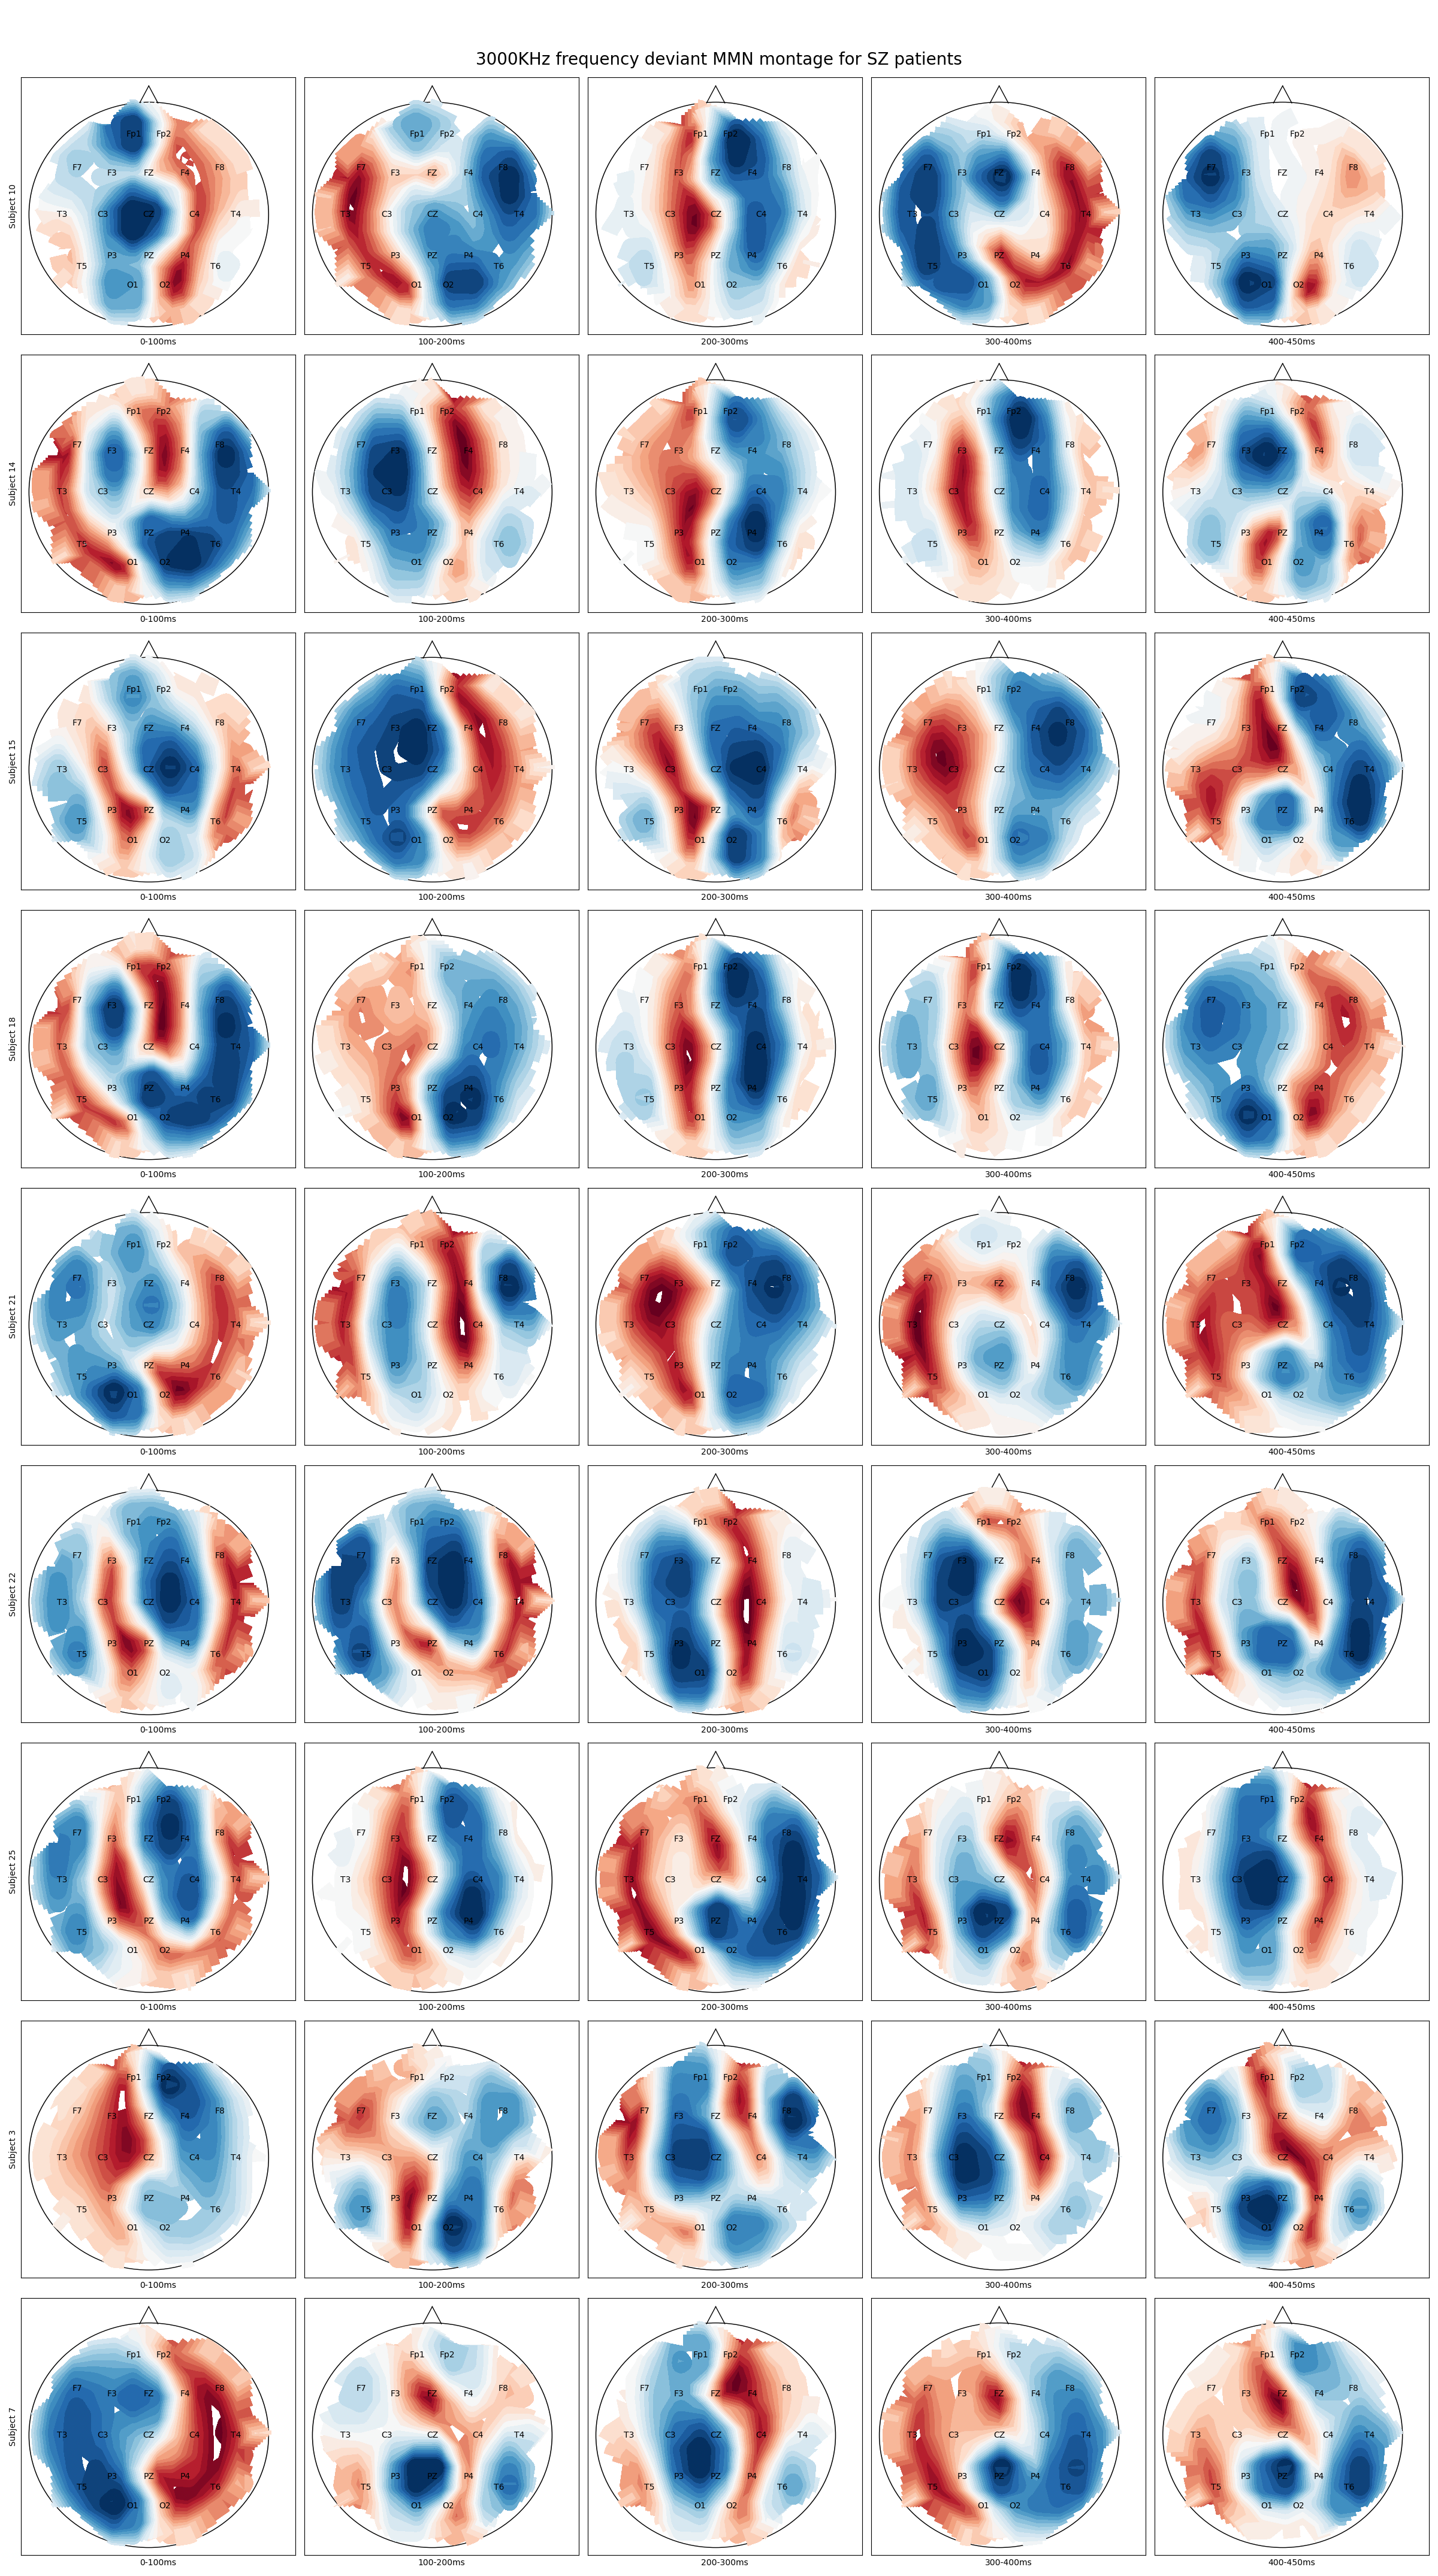
\includegraphics[width=16cm]{../../../data_analysis_results/MMN/montage/Patient/3KHz_frequency_deviant_montage.png}
  \caption{Patients 3KHz frequency deviant \gls{mmn} value montage}\label{patient_3KHz_mmn_montage}
\end{figure}

\begin{figure}[H]
  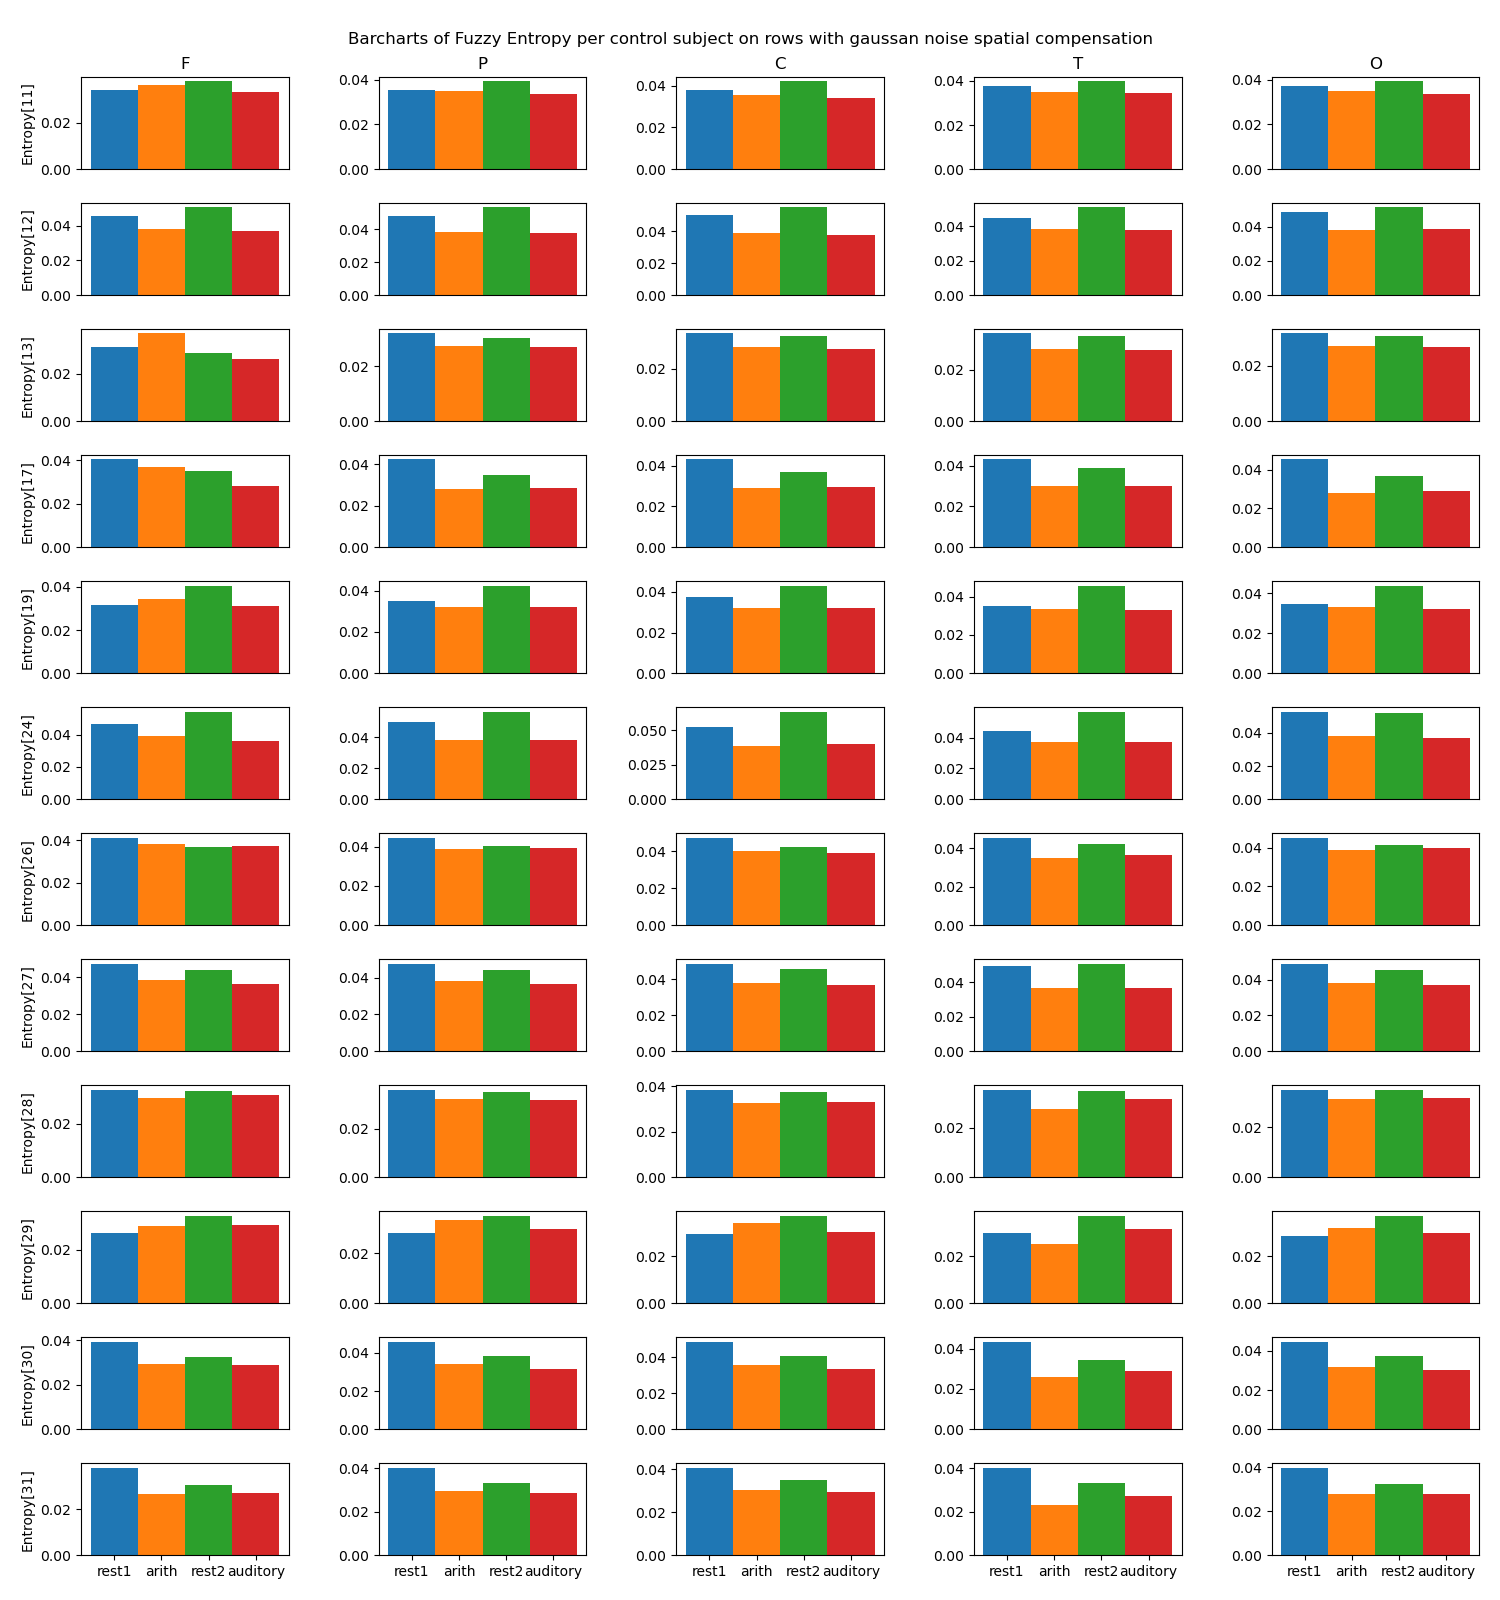
\includegraphics[width=16cm]{../../../data_analysis_results/FuzzEnt/Control/all-fuzzyEntr.png}
  \caption{Fuzzy Entropy from controls}\label{fig:controlFuzzEnt}
\end{figure}
\begin{figure}[H]
  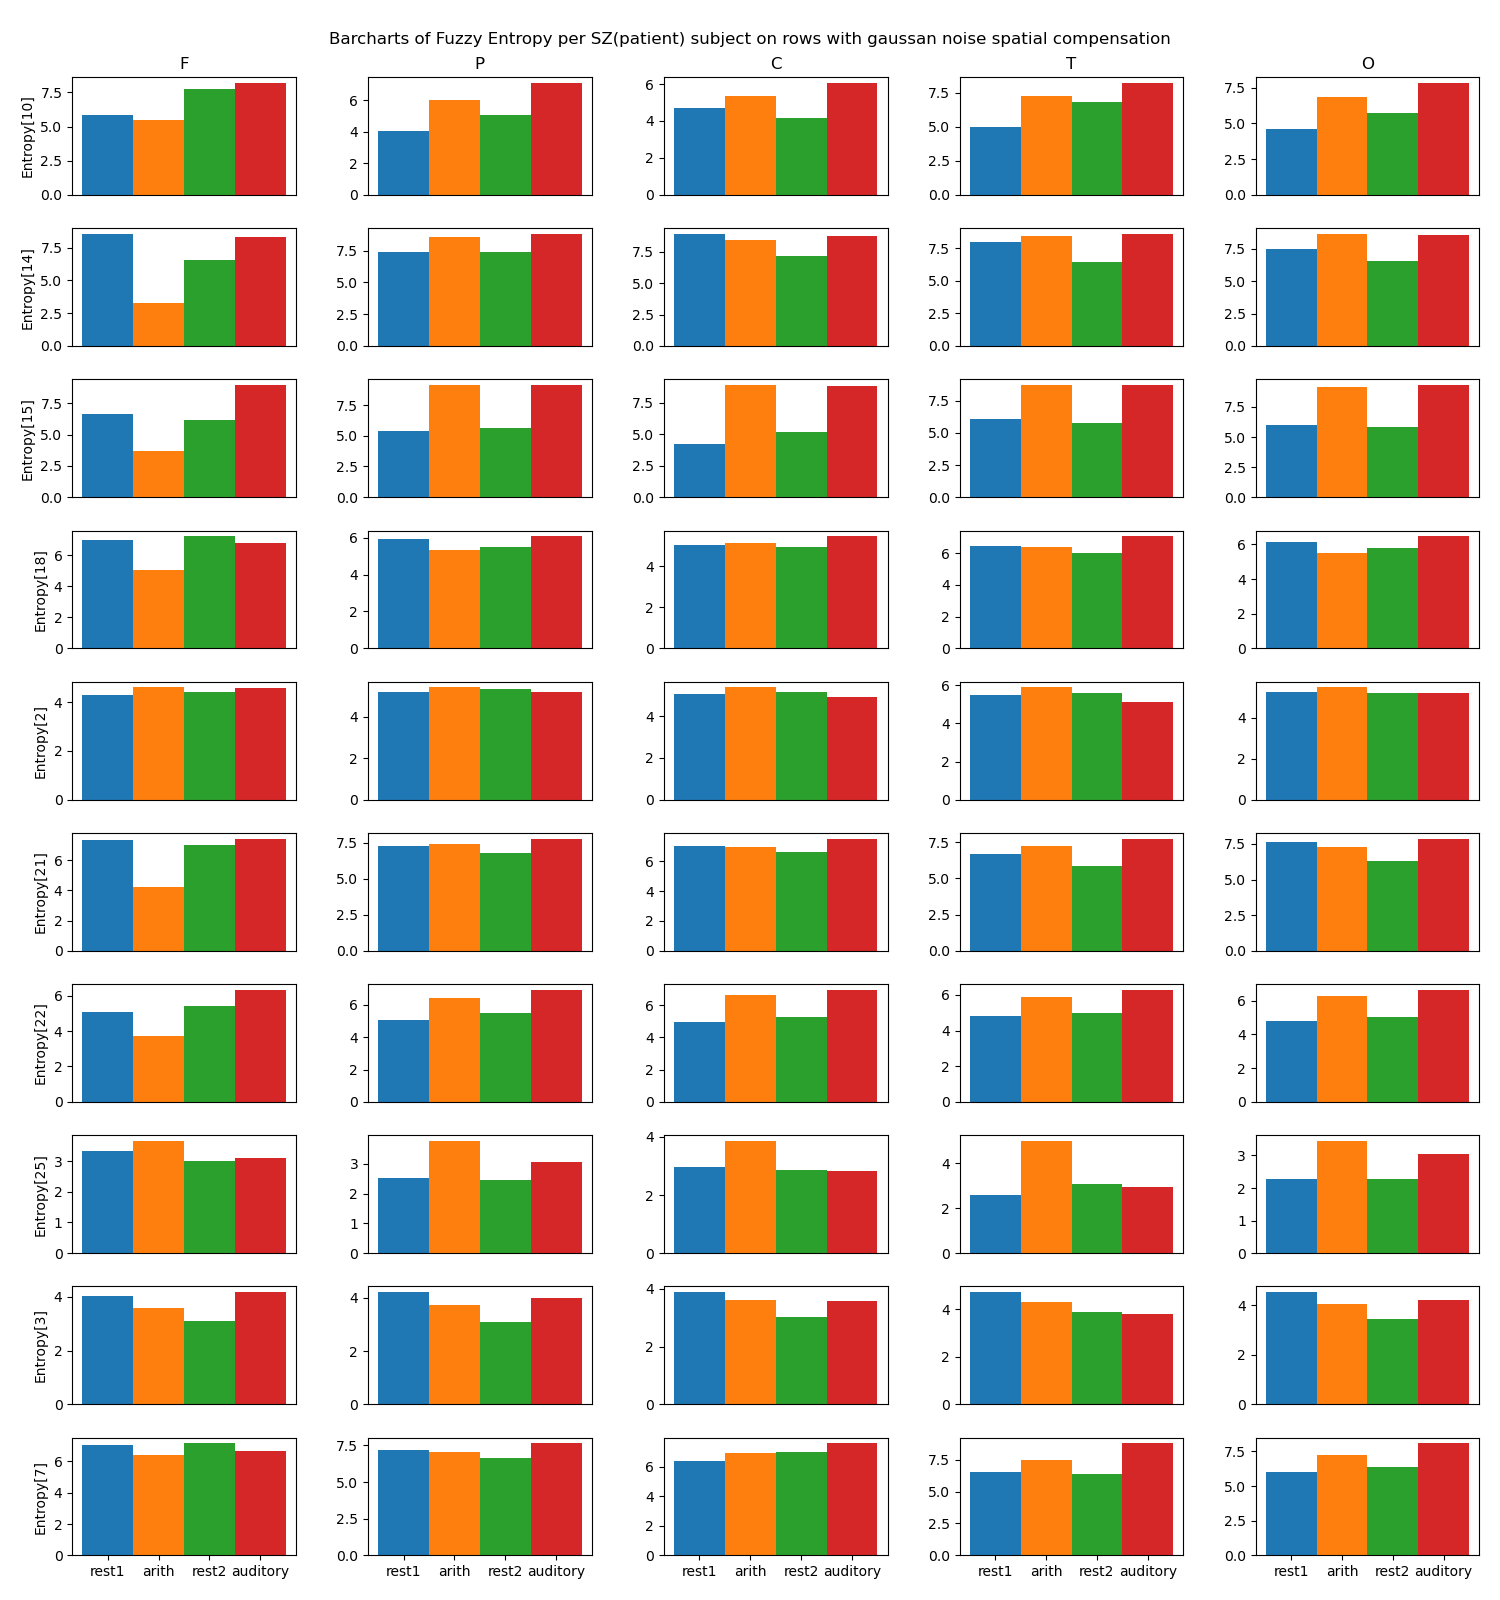
\includegraphics[width=16cm]{../../../data_analysis_results/FuzzEnt/Patient/all-fuzzyEntr.png}
  \caption{Fuzzy Entropy from patients}\label{fig:patientFuzzEnt}
\end{figure}
\begin{figure}[H]
  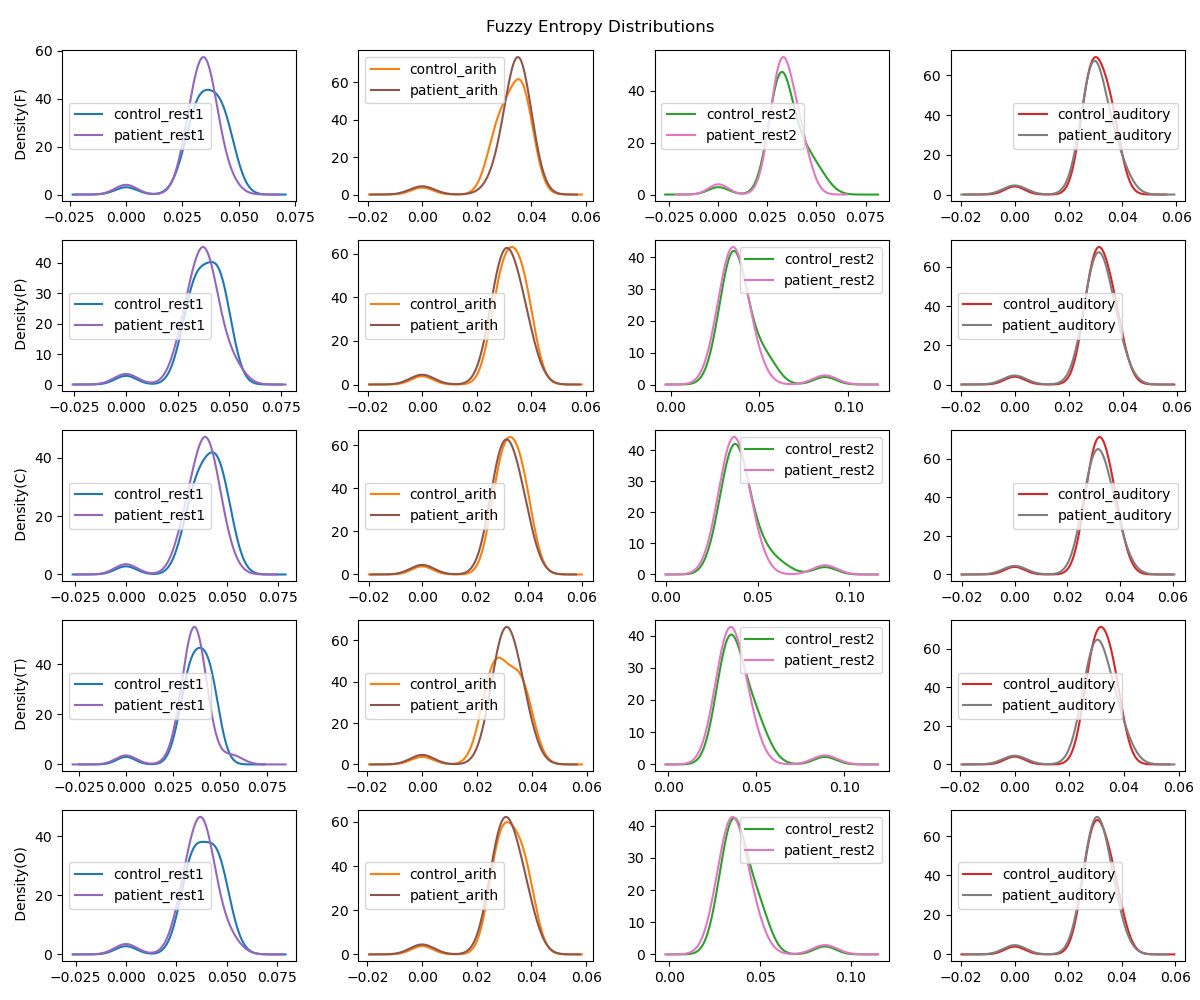
\includegraphics[width=16cm]{../../../data_analysis_results/FuzzEnt/corticalRegions_DAQphase_distributions.png}
  \caption{Fuzzy Entropy from controls}\label{fuzz_ent_distributions}
\end{figure}

\begin{figure}[H]
  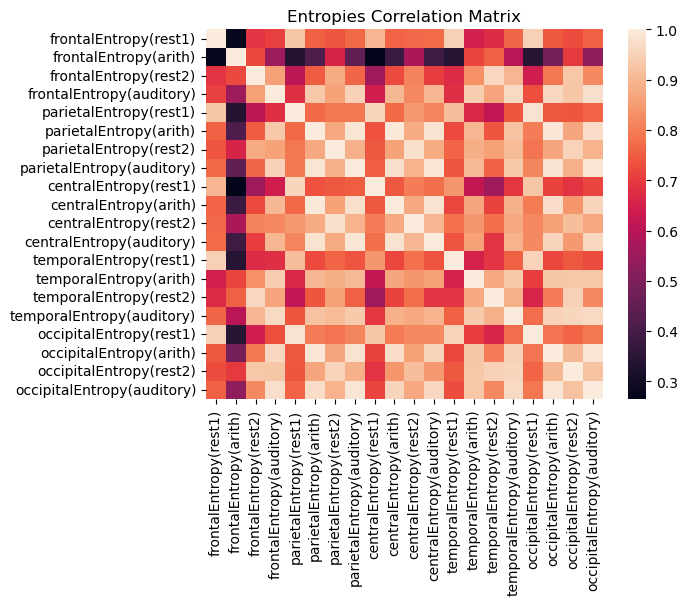
\includegraphics[width=16cm]{../../../data_analysis_results/FuzzEnt/entropies_corr_mat.png}
  \caption{Fuzzy-entropy values correlation smatrix}\label{fuzz_ent_corr_mat}
\end{figure}

\begin{figure}[H]
  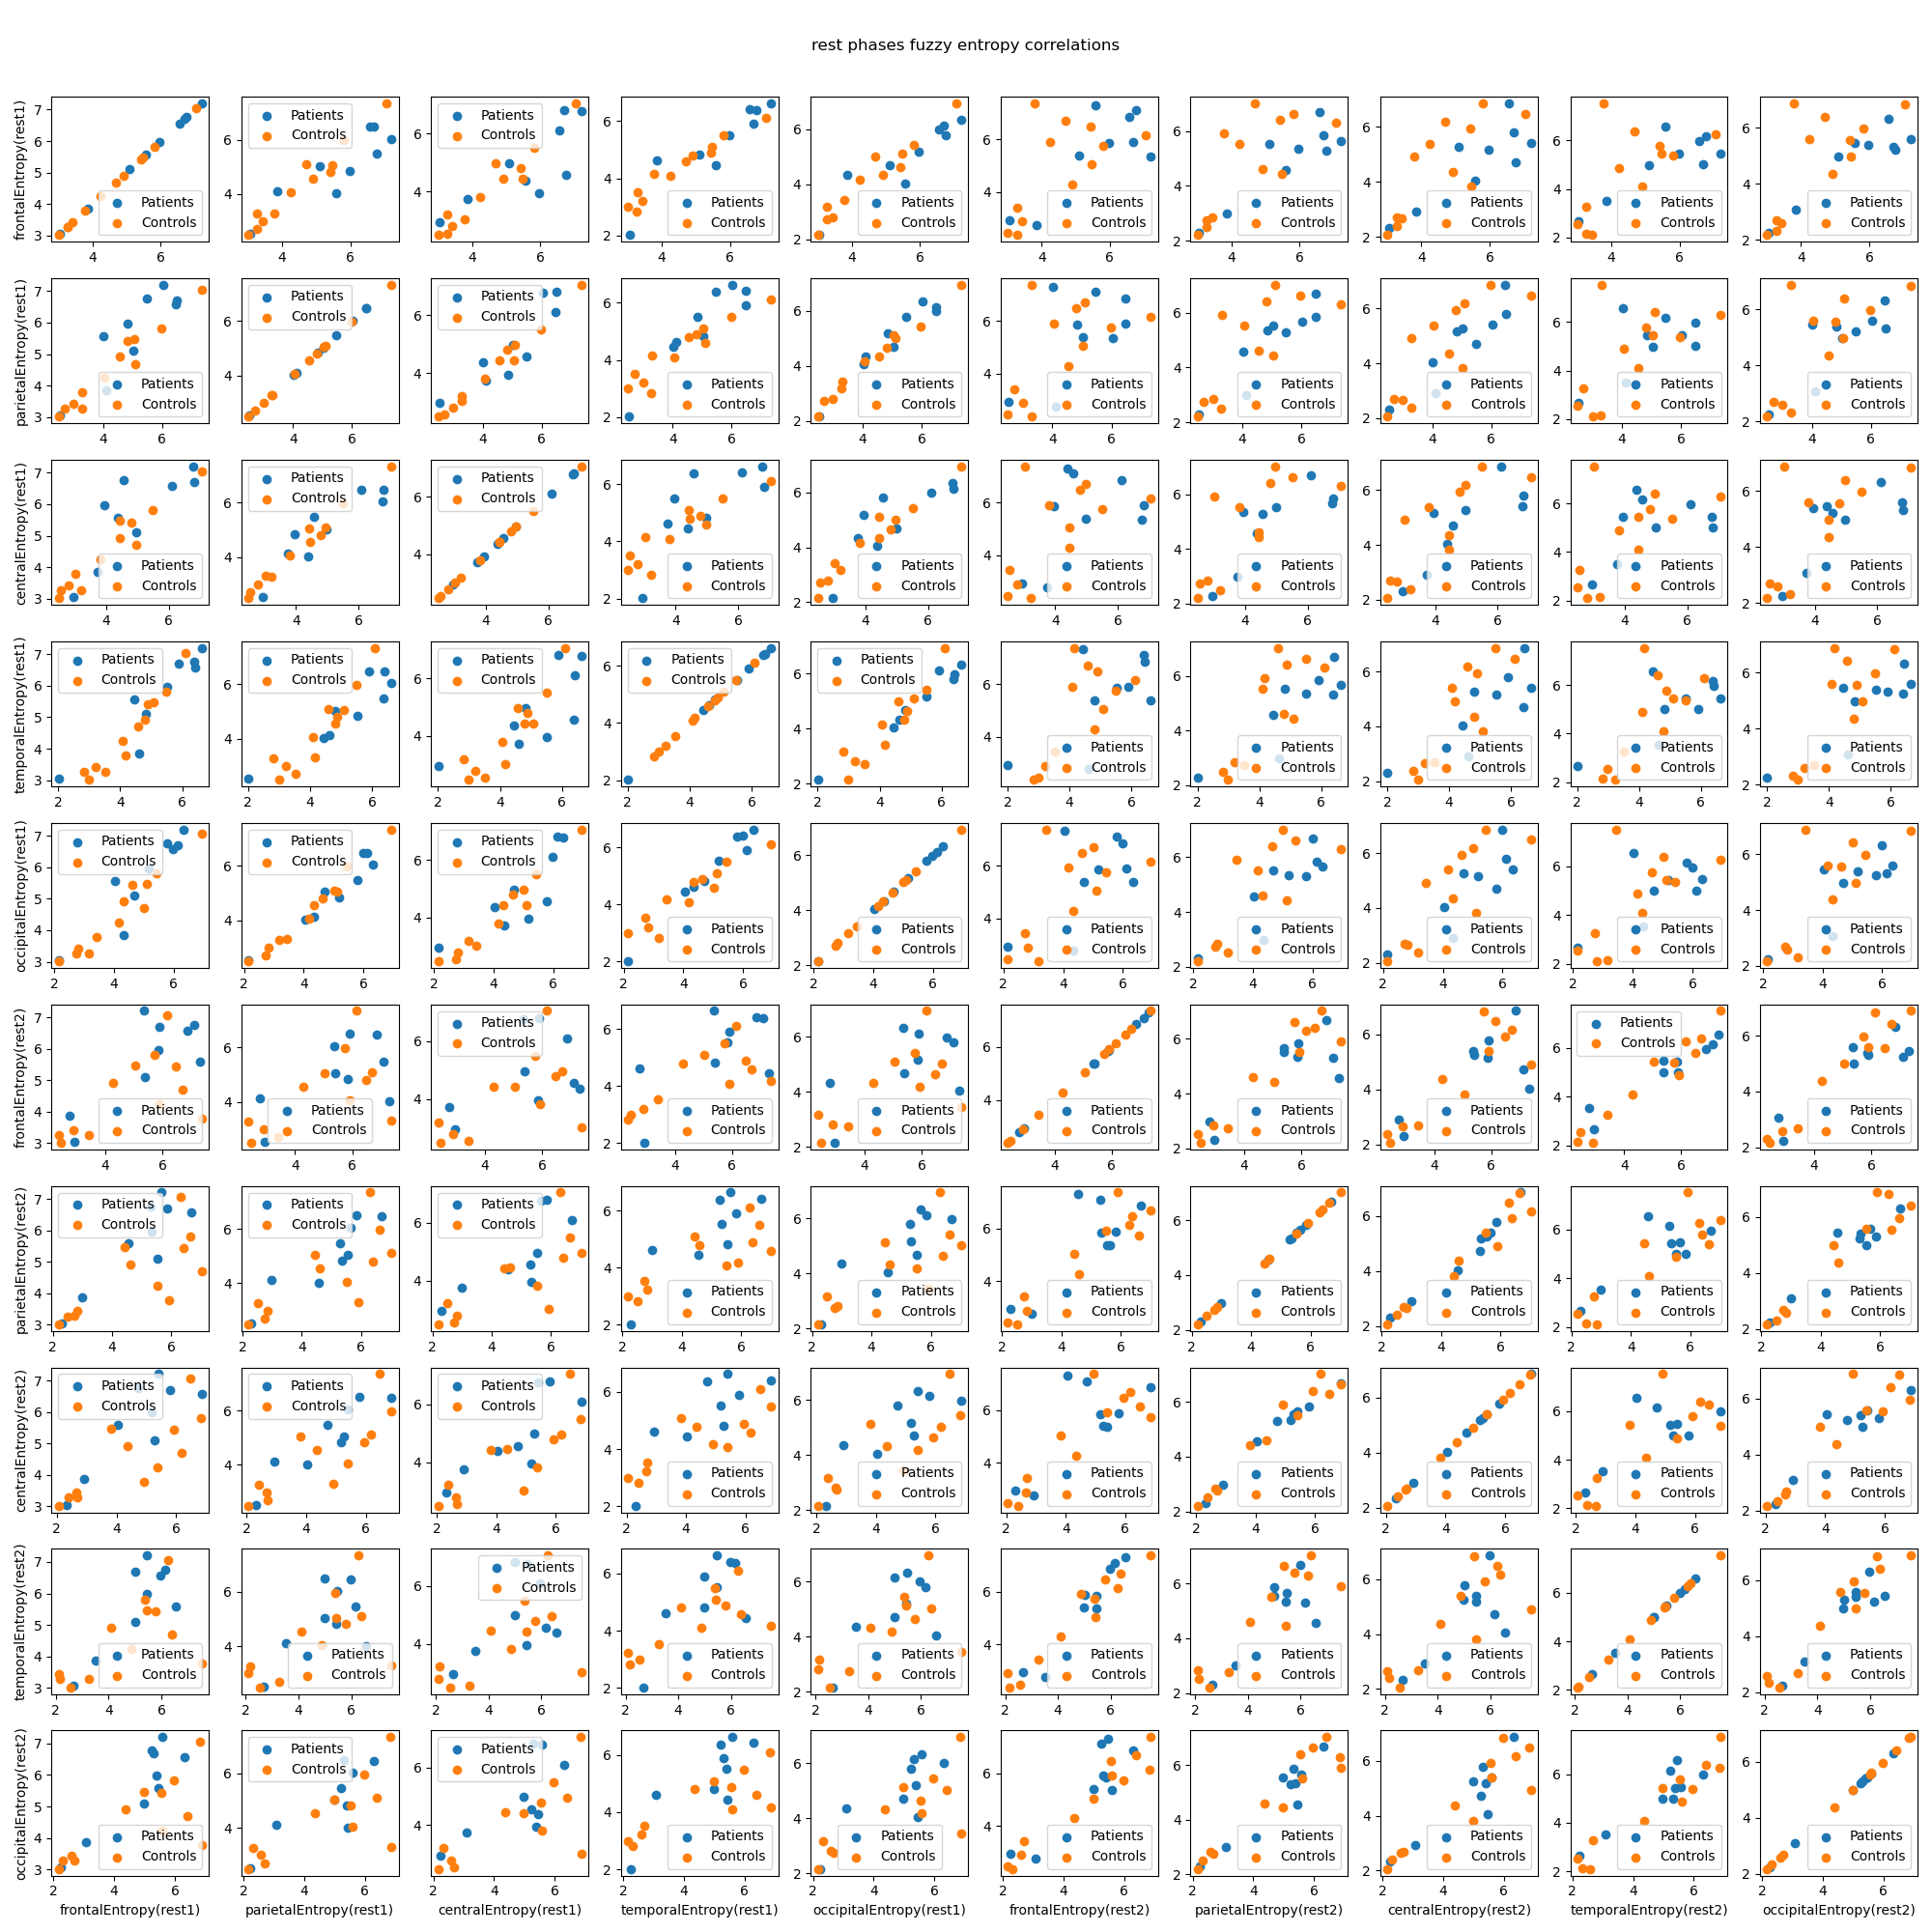
\includegraphics[width=16cm]{../../../data_analysis_results/FuzzEnt/rest_phases_corr.png}
  \caption{Rest Phases Fuzzy-entropy}\label{rest_fuzz}
\end{figure}
\begin{figure}[H]
  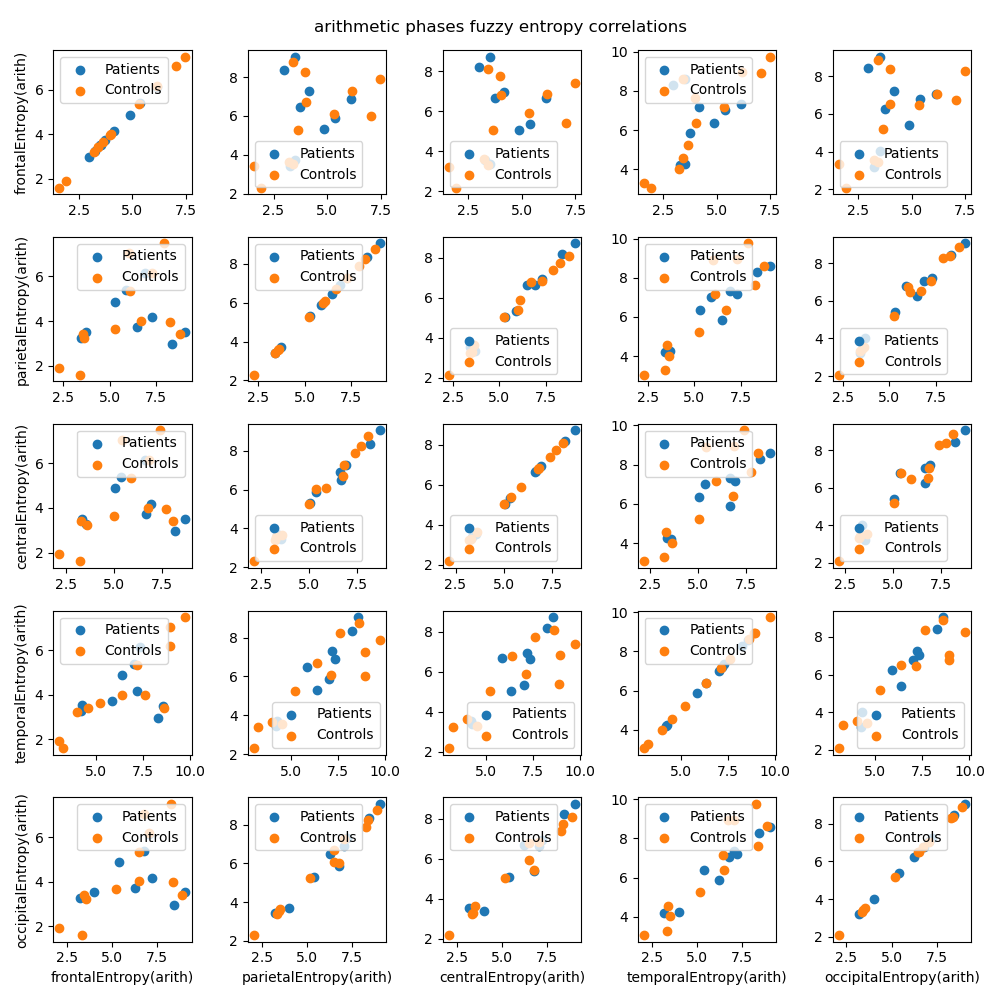
\includegraphics[width=16cm]{../../../data_analysis_results/FuzzEnt/arith_phases_corr.png}
  \caption{Arithmetic Phase Fuzzy-entropy}\label{arith_fuzz}
\end{figure}
\begin{figure}[H]
  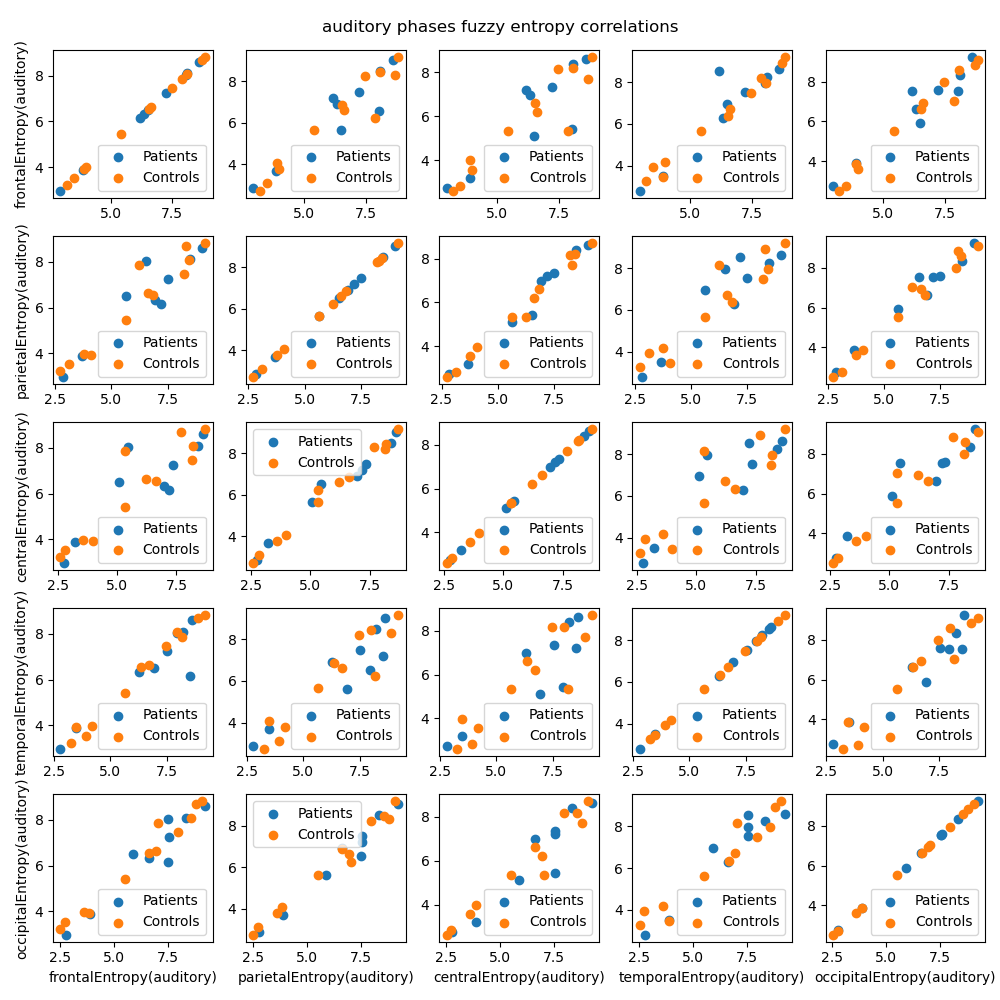
\includegraphics[width=16cm]{../../../data_analysis_results/FuzzEnt/auditory_phases_corr.png}
  \caption{Auditory Phase Fuzzy-entropy}\label{auditory_fuzz}
\end{figure}

\begin{figure}[H]
  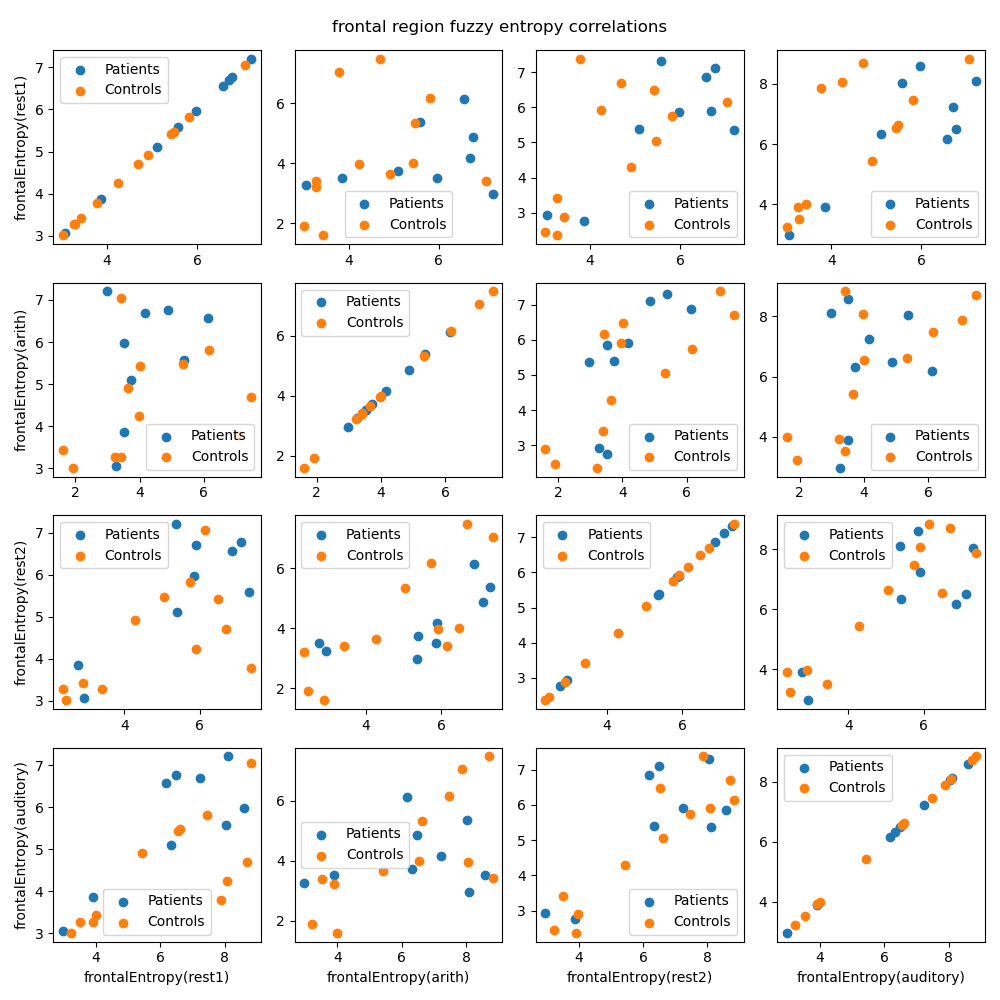
\includegraphics[width=16cm]{../../../data_analysis_results/FuzzEnt/frontal_region_corr.png}
  \caption{Frontal lobe Fuzzy-entropy}\label{frontal_fuzz}
\end{figure}
\begin{figure}[H]
  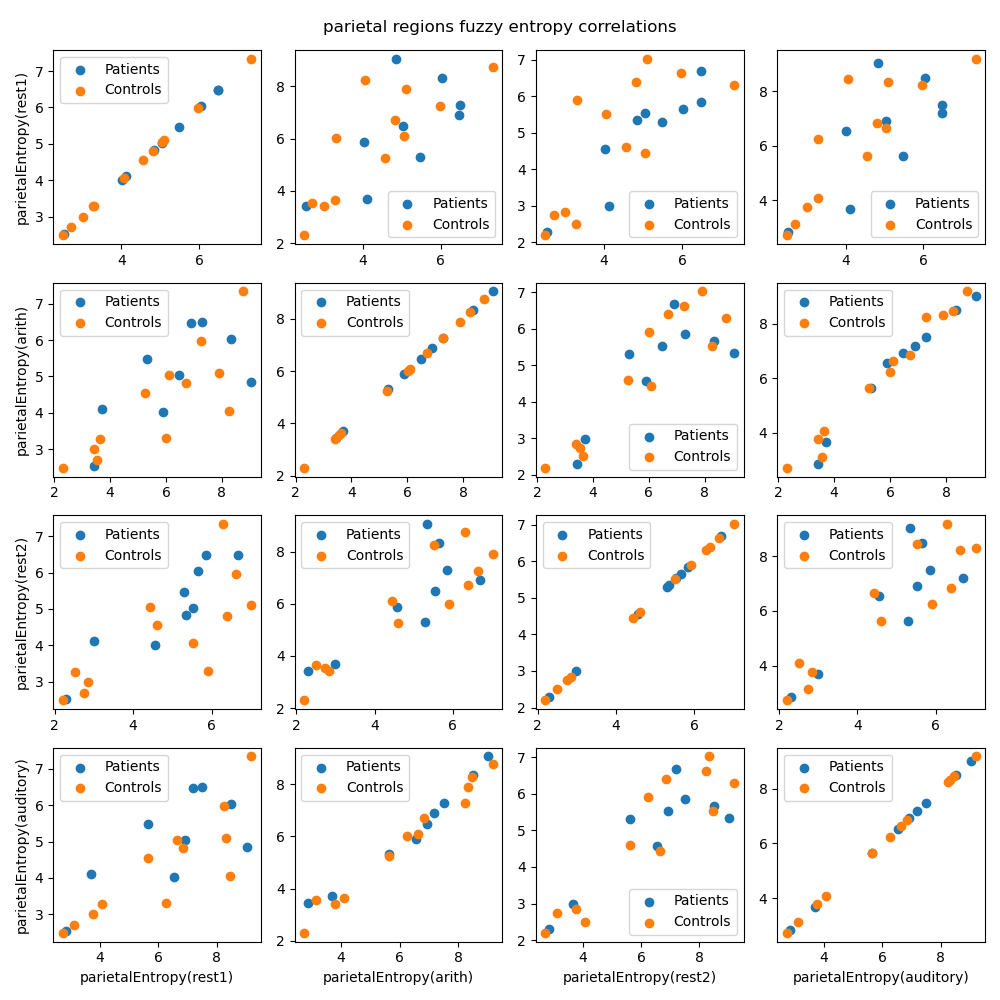
\includegraphics[width=16cm]{../../../data_analysis_results/FuzzEnt/parietal_region_corr.png}
  \caption{Parietal lobe Fuzzy-entropy}\label{parietal_fuzz}
\end{figure}
\begin{figure}[H]
  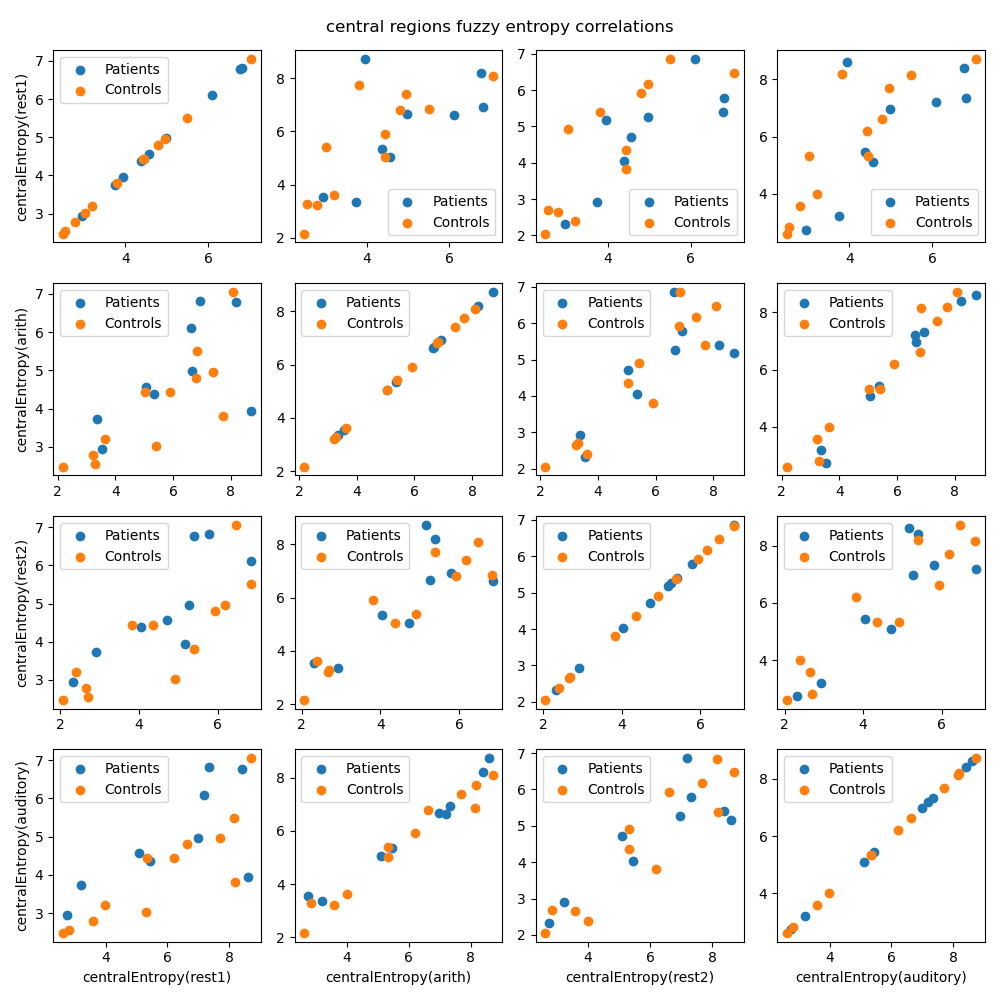
\includegraphics[width=16cm]{../../../data_analysis_results/FuzzEnt/central_region_corr.png}
  \caption{Central lobe Fuzzy-entropy}\label{central_fuzz}
\end{figure}
\begin{figure}[H]
  \includegraphics[width=16cm]{../../../data_analysis_results/FuzzEnt/occipital_region_corr.png}
  \caption{Occipital lobe Fuzzy-entropy}\label{occipital_fuzz}
\end{figure}
\begin{figure}[H]
  \includegraphics[width=16cm]{../../../data_analysis_results/FuzzEnt/temporal_region_corr.png}
  \caption{Temporal lobe Fuzzy-entropy}\label{temporal_fuzz}
\end{figure}

\end{document}
% \include{monthlly_report.acn}

%\journal{CSc 4110 Final Report}

%\title[journalExample]{Format for Project Reports}
\title{
  An update on the project: 
  \textbf{
      \textit{
        Development of an Automatic Instrument for Schizophrenia(SZ) Diagnosis
        }
      }, for the MCIP Innovation Prize 2022.
  }
% \author{
% Emmanuel OLATEJU \\
%     \begin{affiliation}
%       Supervised by Dr. K.P. Ayodele \\ 14/02/2023, \\
%       email: \mbox{kayodele@gmail.com, eoolateju@student.oauife.edu.ng}
%     \end{affiliation}
% }

\begin{document}
\maketitle

\section{Overview}
The purpose of this project is to design an instrument for early \gls{sz} diagnosis.
In designing the instrument, the following parts are to be developed:
\begin{itemize}
  \item An \gls{eeg} \gls{daq} system
  \item \gls{daq} user interface.
  \item Hand-clicker device for \gls{daq} process feedback from patient and clinicians.
  \item Machine/deep learning model.
  \item Soft instrument interacting with learnt model, \gls{daq} software, handheld 
  clicker, \gls{eeg} headbox and all developed parts.
  
\end{itemize}
The goal is to develop a medical turnkey device for \gls{sz} diagnosis having its own 
\gls{eeg} device and deeply embedded software. The long-term goal is for this turnkey device 
and its software to be built around the OpenBCI \gls{eeg} kit. The OpenBCI is chosen as
minimal number of electrode sites needed for \gls{sz} diagnosis may be identified and thus 
an \gls{eeg} kit that allows for flexibility of electrodes to be used is needed. This will 
mitigate the cost of the device making it more accessible. In the short term, the contec 
\gls{eeg} headbox is being used in identifying the best electrode sites.

The contec \gls{eeg} headbox is being used in place of the OpenBCI headbox temporarily 
for generation of the \gls{eeg} signals.
In order to fetch \gls{eeg} signals from the headbox, a piece of software that interacts 
with the contec's firmware has been developed. This piece of software has been incorporated 
with a user interface developed that makes \gls{daq} sessions interactive for both 
subjects and clinicians. The user interface and firmware interacting code together make 
up the Generis software presented in the first report.

In order to make \gls{daq} sessions more interactive, a handheld clicker is being developed 
to help patients and clinicians give feedback to the Generis software. Annotations can be 
somewhat a tough technical task and in certain cases becomes an headache for non-technical 
users. Once annotation messagess are configured into this clicker device, adding annotations 
will be redced to a task of simply clicking color coded buttons. This piece of hardware 
will also improve processing of signals as time during \gls{daq} of noise causing actions can be 
annotated and also times of subject inactivity or inert state to \gls{daq}. The handheld clicker 
is able to communicate with the Generis software through UART to USB communication.

In order to have an instrument of high accuracy and to solve the problem of \gls{sz} diagnosis 
being based on psychiatric nosology, the instrument(model) must be calibrated to seperate 
\glspl{szPtnt} from \glspl{hc}. This is being done using machine-learning and/or 
deep-learning methods and signal-processing algorithms to extract information relevant to 
\gls{sz} measurement and to improve discriminability.

The final instrument that integrates all of the designed parts is to be devloped upon 
completion of the handheld clicker and complete development of model to be used in 
measuring the extent of \gls{sz} disorder and classification of subjects. The structure 
of the final instrument is shown in the diagram below.
\begin{figure}[H]
  \includegraphics[width=16cm]{../../../images/technical/instrument.drawio.png}
  \caption{\gls{sz} diagnosis instrument}\label{instrument}
\end{figure}


\section{Handheld clicker}
The handheld clicker design is based on an arduino nano which applies the output of four 
tact switches as inputs to four vectored interrupts on the nano development board. The 
exact labels of these inputs has not been assigned as a study of the erogonomics of 
conventions employed in other devices of this kind and how best conventions are adapted and 
modified for the use case of this project is being studied. 

The current design of the handheld clicker(annotator) is the second iteration and is referred 
to as HC-v0.2. 
The circuit diagram of the handheld clicker is given in figure \ref{clicker_circuit}.
The flowchart describing the algorithm of this device is shown in figure \ref{clicker_flowchart}. 
The front and top images of the hand-clicker-v0.2 are shown in figures \ref{clicker} and 
\ref{top_view_of_clicker}.
\begin{figure}[H]
  \includegraphics[width=16cm]{../../../hardware/handheld_clicker/circuit_image.png}
  \caption{handheld clicker circuit}\label{clicker_circuit}
\end{figure}
\begin{figure}[H]
  \includegraphics[height=16cm,width=10cm]{../../../hardware/handheld_clicker/flowchart.png}
  \caption{Flowchart algorithm of clicker}\label{clicker_flowchart}
\end{figure}
\begin{figure}[H]
  \includegraphics[width=16cm]{../../../hardware/handheld_clicker/front.jpeg}
  \caption{Front view of clicker}\label{clicker}
\end{figure}
\begin{figure}[H]
  \includegraphics[,height=10cm,width=8cm]{../../../hardware/handheld_clicker/top.jpeg}
  \caption{Top view of clicker}\label{top_view_of_clicker}
\end{figure}


\section{Model Development (Feature-extraction, Data-analysis)}
\subsection{Feature Extraction}
March's report presented the fuzzy entropy features extracted from cortical
regions during phases of \gls{daq} and also the refined \gls{mmn} plots which 
made the \gls{mmn} waveform more evident. Relevant changes made to features 
extraction highlighted in marchs's report includes:
\begin{itemize}
  \item Recomputing the \gls{mmn} waveforms
  \item Spatial dimension augmentation with gaussian noise during computation of fuzzy-entropy
  \item Development of custom fuzzy-entropy library
\end{itemize}
The following was proposed as the next set of action points:
\begin{itemize}
  \item The continued improvement of fuzzy-entropy library to work with multivariate \\
  time-series(2D data)
  \item comparing performance of the fuzzy-entropy features from sourced library to \\
  that of the personally developed library
  \item Computing the auditory steady state features
\end{itemize}
A slight detour was made from these proposed action points for the month of april. 
Analysis of the extracted features for levels of dicriminability was carried out 
to understand how to improve the features extraction methods. The analysis shows 
a significant level of discrimination in the \gls{mmn} features, less in the 
fuzzy-entropy features, though the correlation patterns of the fuzzy-entropy features 
suggest they might carry information on extent of \gls{sz} disorder.

\gls{mmn} features have been extracted from the scaled \gls{mmn} waveforms. The 
\gls{mmn} features were computed as the mean of the \gls{mmn} waveforms within 
the time-frames 0-100ms, 100-200ms, 200-300ms, 300-400ms, 400-450ms.

Formerly implemented montage plot algorithm was improved upon to reduce 
time-complexity so as to make data visualization and analysis easier to obtain 
intuitive information from.

\subsection{Data Analysis/Visualization}\label{data_analyis}
 Analysis of the extracted features was done to establish the quality of discriminative 
 and quantitative information contained in the extracted features. The method of 
 Visualization of some of these features changed to make analysis easy.
 The results of the analysis are given in section \ref{figures}. Visualization methods 
 and analysis carried out includes:
\begin{itemize}
  \item Comparing \gls{mmn} feature values for 1KHz duration deviant and 3KHz frequency deviant 
  between patient and controls across all electrodes and time windows.
  (Figures \ref{mmnvalue_0_100ms} - \ref{mmnvalue_400_450ms})
  \item Converting the \gls{mmn} values to montage plots for 1KHz duration deviant 
  and 3KHz frequency deviant for easier interpretation and analyzing montage evolution.
  (Figures \ref{control_1KHz_mmn_montage}-\ref{patient_3KHz_mmn_montage})
  \item Comparing distribution of computed fuzzy-entropy values of patients and controls 
  for each cortical region across all phases of \gls{daq}.
  (Figures \ref{fig:controlFuzzEnt}-\ref{fuzz_ent_distributions}) 
  \item Correlating fuzzy-entropy values from cortical regions across 
  all phases of \gls{daq}.(Figure \ref{fuzz_ent_corr_mat})
  \item Comparing entropies from all cortical regions for each phase of \gls{daq}.
  (Figures \ref{rest_fuzz}-\ref{auditory_fuzz})
  \item Comparing entropies from all phases of \gls{daq} for each cortical region.
  (figures \ref{frontal_fuzz}-\ref{temporal_fuzz})
\end{itemize} 

\section{Inference and Action Points}
\subsection{Inference}
From the analysis carried out, the \gls{mmn} features of both tone deviants show 
discriminative properties between the \gls{szPtnt} and \gls{hc} in localized head 
regions. The fuzzy-entropy features do not show discriminative abilities, but their 
correlation patterns indicate a linear relationship that might be a measure of degree 
of \gls{sz} disorder. Therefore we need to find methods that improve quality of extracted 
features and proceed with developing a learner model.

\subsection{Action Points}
Based on the inference drawn, the action points for the month of may is as follows:
\begin{itemize}
  \item Computing the auditory steady state features.
  \item Re-computing fuzzy-entropy features using other libraries and 
  comparing performance.
  \item Improve discriminability of features using spatial filters and dimensionality 
  reduction techniques.
  \item Compare performance of a custom mutilayer feedforward network and traditional 
  machine-learning algorithms for classification and estimation of measures of degree 
  of \gls{sz} disorder.
\end{itemize}

\section{Figures}\label{figures}

\begin{figure}[H]
  \includegraphics[width=16cm]{../../../data_analysis_results/MMN/features/deviant_tone_0.png}
  \caption{\gls{mmn} values from 0-100ms}\label{mmnvalue_0_100ms}
\end{figure}
\begin{figure}[H]
  \includegraphics[width=16cm]{../../../data_analysis_results/MMN/features/deviant_tone_1.png}
  \caption{\gls{mmn} values from 100-200ms}\label{mmnvalue_100_200ms}
\end{figure}
\begin{figure}[H]
  \includegraphics[width=16cm]{../../../data_analysis_results/MMN/features/deviant_tone_2.png}
  \caption{\gls{mmn} values from 200-300ms}\label{mmnvalue_200_300ms}
\end{figure}
\begin{figure}[H]
  \includegraphics[width=16cm]{../../../data_analysis_results/MMN/features/deviant_tone_3.png}
  \caption{\gls{mmn} values from 300-400ms}\label{mmnvalue_300_400ms}
\end{figure}
\begin{figure}[H]
  \includegraphics[width=16cm]{../../../data_analysis_results/MMN/features/deviant_tone_4.png}
  \caption{\gls{mmn} values from 400-450ms}\label{mmnvalue_400_450ms}
\end{figure}

\begin{figure}[H]
  \includegraphics[width=16cm]{../../../data_analysis_results/MMN/montage/Control/1KHz_duration_deviant_montage.png}
  \caption{Controls 1KHz duration deviant \gls{mmn} value montage}\label{control_1KHz_mmn_montage}
\end{figure}
\begin{figure}[H]
  \includegraphics[width=16cm]{../../../data_analysis_results/MMN/montage/Patient/1KHz_duration_deviant_montage.png}
  \caption{Patients 1KHz duration deviant \gls{mmn} value montage}\label{patient_1KHz_mmn_montage}
\end{figure}
\begin{figure}[H]
  \includegraphics[width=16cm]{../../../data_analysis_results/MMN/montage/Control/3KHz_frequency_deviant_montage.png}
  \caption{Controls 3KHz frequency deviant \gls{mmn} value montage}\label{control_3KHz_mmn_montage}
\end{figure}
\begin{figure}[H]
  \includegraphics[width=16cm]{../../../data_analysis_results/MMN/montage/Patient/3KHz_frequency_deviant_montage.png}
  \caption{Patients 3KHz frequency deviant \gls{mmn} value montage}\label{patient_3KHz_mmn_montage}
\end{figure}

\begin{figure}[H]
  \includegraphics[width=16cm]{../../../data_analysis_results/FuzzEnt/Control/all-fuzzyEntr.png}
  \caption{Fuzzy Entropy from controls}\label{fig:controlFuzzEnt}
\end{figure}
\begin{figure}[H]
  \includegraphics[width=16cm]{../../../data_analysis_results/FuzzEnt/Patient/all-fuzzyEntr.png}
  \caption{Fuzzy Entropy from patients}\label{fig:patientFuzzEnt}
\end{figure}
\begin{figure}[H]
  \includegraphics[width=16cm]{../../../data_analysis_results/FuzzEnt/corticalRegions_DAQphase_distributions.png}
  \caption{Fuzzy Entropy from controls}\label{fuzz_ent_distributions}
\end{figure}

\begin{figure}[H]
  \includegraphics[width=16cm]{../../../data_analysis_results/FuzzEnt/entropies_corr_mat.png}
  \caption{Fuzzy-entropy values correlation smatrix}\label{fuzz_ent_corr_mat}
\end{figure}

\begin{figure}[H]
  \includegraphics[width=16cm]{../../../data_analysis_results/FuzzEnt/rest_phases_corr.png}
  \caption{Rest Phases Fuzzy-entropy}\label{rest_fuzz}
\end{figure}
\begin{figure}[H]
  \includegraphics[width=16cm]{../../../data_analysis_results/FuzzEnt/arith_phases_corr.png}
  \caption{Arithmetic Phase Fuzzy-entropy}\label{arith_fuzz}
\end{figure}
\begin{figure}[H]
  \includegraphics[width=16cm]{../../../data_analysis_results/FuzzEnt/auditory_phases_corr.png}
  \caption{Auditory Phase Fuzzy-entropy}\label{auditory_fuzz}
\end{figure}

\begin{figure}[H]
  \includegraphics[width=16cm]{../../../data_analysis_results/FuzzEnt/frontal_region_corr.png}
  \caption{Frontal lobe Fuzzy-entropy}\label{frontal_fuzz}
\end{figure}
\begin{figure}[H]
  \includegraphics[width=16cm]{../../../data_analysis_results/FuzzEnt/parietal_region_corr.png}
  \caption{Parietal lobe Fuzzy-entropy}\label{parietal_fuzz}
\end{figure}
\begin{figure}[H]
  \includegraphics[width=16cm]{../../../data_analysis_results/FuzzEnt/central_region_corr.png}
  \caption{Central lobe Fuzzy-entropy}\label{central_fuzz}
\end{figure}
\begin{figure}[H]
  \includegraphics[width=16cm]{../../../data_analysis_results/FuzzEnt/occipital_region_corr.png}
  \caption{Occipital lobe Fuzzy-entropy}\label{occipital_fuzz}
\end{figure}
\begin{figure}[H]
  \includegraphics[width=16cm]{../../../data_analysis_results/FuzzEnt/temporal_region_corr.png}
  \caption{Temporal lobe Fuzzy-entropy}\label{temporal_fuzz}
\end{figure}

\end{document}
% \include{monthlly_report.acn}

%\journal{CSc 4110 Final Report}

%\title[journalExample]{Format for Project Reports}
\title{
  An update on the project: 
  \textbf{
      \textit{
        Development of an Automatic Instrument for Schizophrenia(SZ) Diagnosis
        }
      }, for the MCIP Innovation Prize 2022.
  }
% \author{
% Emmanuel OLATEJU \\
%     \begin{affiliation}
%       Supervised by Dr. K.P. Ayodele \\ 14/02/2023, \\
%       email: \mbox{kayodele@gmail.com, eoolateju@student.oauife.edu.ng}
%     \end{affiliation}
% }

\begin{document}
\maketitle

\section{Summary}\label{sec:summary}
  As stated in the proposal document, this project came about as a result 
  of the lack of a pre-psychotic objective scientific instrument to diagnose 
  \gls{sz}, this poses a large social threat as exiting nosologyis based 
  on psychiatric evaluation requires active psychosis after which epidemiology 
  becomes difficult and expensive to manage, thus the need to develop 
  an instrument for early detection of \gls{sz} This project aims to 
  develop a classifier for early detection of schizophrenics using the 
  \gls{assr}, fuzzy entropy and \gls{mmn}
  features from \gls{eeg} data of subjects. 

  In order to achieve the aforemntioned aim, data has been acquired 
  from a total of 31 subjects divided into the \glspl{hc} and \glspl{szPtnt}, 
  of which 13 are \glspl{hc} and 18 are \glspl{szPtnt} 
  After dropping null EEG recordings, the resulting data was made up of 10 
  \glspl{szPtnt} and 12 \glspl{hc}, a total of 22 subjects out of 31. Data 
  acquisition is done using the contek KT-2400 and KT-1018 devices of 
  sampling rates 200Hz and 100Hz respectively. The KT-1018 was used mainly 
  in testing of the developed software for data acquisition called Generis. 
  \Gls{daq} and the Generis software are discussed within section \ref{sec:DAQ} 
  of this document.
  

  First outlook at \gls{dtpcn} produced \gls{eeg} spatial and time-domain 
  resulsts. Valid data from the 22 subjects have been subjected to a different 
  \gls{dtprepcn} and \gls{dtpcn} pipeline producing results in the time, 
  time-frequency domain and giving measures of disorderliness of spatial 
  collapsed spatio-temporal series. These methods are discussed under section 
  \ref{sec:processing} of this document.

  After processing, plots of results showed certain distinct characteristics 
  between the \glspl{hc} and \glspl{szPtnt}. These differences 
  are discussed under section \ref{sec:re} of this document and 
  figures describing such differences are shown in section \ref{se:figures} of 
  this document.

  This report also documents the milestones achieved, the challenges faced and 
  the next steps towards achieving the aim of this project. This steps definitely 
  do include more \gls{daq} and making \gls{dtpcn} more robust.
  %Timelines are 
  %attached alongside the next steps towards achieving the aim of developing an 
  % instrument for \gls{sz} diagnosis.









\section{Data Acquisition}\label{sec:DAQ}
This section will discuss the \gls{eeg} devices used for acquisition, the 
acquisition protocol, phases of \gls{daq} protocol and their modalities. Lastly 
this section will briefly review the Generis software developed for \gls{daq}, as 
an holistic approach in explaining this software can be time consuming as it took 
two programmers to design this software, I being one of the two.

\subsection{Devices}\label{ssce:EEG devices}
\gls{daq} was done using two \gls{eeg} devices from the same 
manufacturer named the KT2400 and KT1018 from contek devices, each having 24 
electrode channels and 18 electrode channels respectively.

The KT-1018 is a 16 channel \gls{eeg} device with a sampling rate of 
\SI{100}{\hertz} per electrode channel. Its electrodes are distributed between 
the frontal, central, temporal, occipital and parietal lobes. The device has an 
\gls{adc} resolution of 12bits with a minimum input impedance of 
\SI{10}{\mega\ohm} and a patient leak current of \SI{10}{\micro\ampere}. Its 
noise parameters are good enough for the use case of this project which include 
a maximum noise level of \SI{5}{\micro\volt} peak to peak, a minimum common mode 
rejection ratio of \SI{90}{\decibel} and a minimum \SI{50}{\hertz} interference 
suppression level of \SI{30}{\decibel}.

The KT-2400 is a 19 channel \gls{eeg} device with similar noise performance 
characteristics to the KT-1018. it also has similar resolution and amplifier, sensor 
electrical parameters. It differs from the KT-1018  in it being a 19 \gls{eeg} electrode 
channel \gls{eeg} device and having a sampling rate of \SI{200}{\hertz} per 
channel.

The two devices have similar performance and similar behaviour in terms of 
communication protocol and mode settings. The KT-1018 was used in developing the 
Generis software initially and was expanded to cater for the KT-2400 later on. All 
data analysed were acquired using the KT-2400 device.

\subsection{Acquisition Protocol}\label{ssec:DAQ protocol}
There is the need to define a protocol to be followed during acquisition, for easy 
identification, interpretaion, analysis and classification of data acquired. The 
\gls{eeg} data is acquired in four phases, the order of which is defined for each 
subject by the acquisition protocol shown in figure \ref{fig:data phases}.

\begin{figure}[H]
  \includegraphics{images/data_phases.png}
  \caption{Order of data phases in acquisition protocol}
  \label{fig:data phases}
\end{figure}

The time frame of acquisition for each phase is still conventional. It has been 
allowed to vary based on judgement of the electrophysiologist in charge of session.
The time values shown in figure \ref{fig:data phases} is that which is most 
common among subjects trials. The method of delivery of the cue 
and instructions in each phase are defined by that phase. This is currently being 
updated based on suggestions from the electrophysiologists.

During the first and second rest phases, the subject receives an instruction to remain calm, 
avoid any form of movements and notify the clinicians and electrophysiologist of any 
inconvenience by means of speech. Instructions are delivered through the sound media output of device running the 
Generis software and displayed  on the screen of the device. The auditory based instruction modality is language specific covering 
English, yoruba, hausa and pidgin, igbo yet to be covered. There is no need for any sort of special cue in these phases. 
The subject is expected to adhere to these instructions all through  these phases. But in the 
case of the subject being a \gls{szPtnt}, such subject might not fully understand the 
instructions and act against instructions, there is the need to annotate such points in time 
in the EEG data as artifact periods. This is currently being catered for by the the design of an hardware annotator.

In the arithmetic phase, instructions are again given via auditory and now visual means 
after which a series of arithmetic task are dictated to the subject by the software in his/her selected language 
and also displayed on the screen. A fixed time is allowed to pass during which the subject is expected 
to attempt the task and give  any answer. An incorrect answer is of no consequence as the arithmetic task, 
acts as an activation energy for the cognitive channels of the brain, so their state which is indicative of 
\gls{sz} status can be investigated. This phase uses no annotations and as such, the point in time 
at which the subject receives(understands) an arithmetic task and gives his/her answer is unknown. This is also catered for in 
the ongoing design of the hardware annotator.

The auditory stimuli phase instructions are similar to that of the rest phase. During this phase, 
the subject listens to a sequence of tones each, with the component tones having different parameters. 
There is the \SI{1}{\kilo\hertz} standard tone, the \SI{3}{\kilo\hertz} frequency deviant tone and the 
duration deviant tone. While listening to these tones, the subject passively wacthes a random clip to 
divert the subjects attention from the tone sequence. Each tone stimuli class lasts for a minimum of 
\SI{100}{\milli\second}. 

Implementation of these phases, their cues, instrucions and annotations is achieved and managed by 
the Generis software which will be discussed next.

The \gls{eeg} data from the auditory stimuli phase is to be used in  computing the \gls{mmn} response.
Fuzzy entropy and \Gls{assr} paraneters are to be computed for \gls{eeg} data of all phases and compared 
for notable differences between the \glspl{hc} and the \glspl{szPtnt}.

\subsection{Generis Softwware}\label{ssec:Generis}
The Generis \gls{daq} software was designed for the following reasons:
\begin{itemize}
  \item For communication with contek firmware to receive \gls{eeg} data stream.
  \item For control of switching between phases and visual/auditory presentation of stimuli and instructions.
  \item For annotating \gls{eeg} data event occurence in time.
  \item For taking in subject, clinician and electrophysiologist feedback/annotation.
  \item For time synchronization of annotation stream, feedback stream and \gls{eeg} stream.
  \item For subject info management.
\end{itemize}

The Generis software is mnade up of components parts which interact with 
themselves to achieve the purpose of the built software which can be 
summarized as event occurence tracking and recording of \gls{eeg} data. 
Figure \ref{fig:Generis Architecure} shows the architecture of the system of which each box represents 
a component part of the software.
\begin{itemize}
  \item Cue generator: The cue generator according to the appropriate \
  phase of \gls{daq} generates cues or instructions information which is passed 
  to the annotator.
  \item Annotator: The annotator based on phase of execution, time of phase and \
  data from the cue genertor generates time/string(marker) information to be attached to 
  the \gls{eeg} recording and stored in its file, the \Gls{edf} file.
  \item USB Driver: This is responsible for fetching the EEG data in its raw
  binary form. This interacts with the firmware on the contek device.
  \item edf maker: This components receives the \gls{eeg} data from the USB driver,\ 
  alongside the sample number from the onset of recording and saves it into a variable \ 
  within the generated \gls{edf} filed called \textit{eeg\_data} and uses the information from 
  the annotator and sample number from recording onset to append to a variable called \textit{eeg\_markers} 
  in the generated \gls{edf} file. Onset of events are represented by their appropriate string and their time of occurence 
  in \gls{eeg} recording. 
  \item Audio/Video module: The audio module based on phase of \gls{daq} and input gotten from annotator \
  selects what pre-recorded audio file of stimuli or instruction is to be played using the laptops media sound 
  output. During the auditory stimuli phase of acquisition, random image clips are combined into frames of a 
  video for the subject to watch. This is implemented by the video module.
  \item GUI: This is the \Gls{gui} module which implements what is seen by the eclectrophysiologist and 
  subject during recording. It allows the electrophysiologist set the recording parameters such as dration 
  for each phase, subject info such as age, religion, language, etc.. It also allows the electrophysiologist 
  select \gls{eeg} recording device to be used. KT-1018 or KT-2400. It has three sub-components namely:
  \begin{itemize}
    \item Instruction screen: which just displays audio  and non-audio instructions in textual form.
    \item Settings screen whch allows clinician/electrophysiologist to interact with software so as to define \
    parameters of recording.
    \item \gls{eeg} display screen which justs plots the acquired EEG data in real time. 
  \end{itemize}
\end{itemize}

The flowchart of the USB driver for acquisition of one sample of data is shown in figure \ref{fig:kt108 sample}.
Figures \ref{fig:acquisitionScreen} through \ref{fig:subjectCreate} shows various interfaces of the Generis software.







\section{Processing}\label{sec:processing}
This section discusses both the preprocessing and processing(feature-computation) of the acquired \gls{eeg} data.
Some results are discussed here with the figures displayed under section \ref{sec:figures} of this document.

\subsection{Preprocessing}\label{ssec:ppcn}
\Gls{dtprepcn} pipeline has been developed to be flexible in order to allow for results comparison 
between the various sequence of methods chosen. The adopted \gls{dtprepcn}  architecture is shown 
in figure \ref{fig:data preprocessing}.

In order to have a first outlook of the acquired data, preprocessing was carried out on the \gls{eeg} data of 
the first three subjects. Montage plots and time-series plot of electrodes of 
the temporal lobe were generated, the time-series plot being from the auditory stimui phase 
\gls{eeg} data. To generate the montage plots, three preprocssing path were tried. One made use of 
1-70Hz bandpass filtering alone, another combined edge interpolation,another combined edge-interpolation 
and baseline correction. Taking the first as the standard, it was observed that without baseline correction, 
edge-inerpolation inverted the spatial domain information shown by the montage plot, while baseline-correction alongside 
edge-interpolation helped recover this information. The figures describing these results are shown in figures 
\ref{fig:montages}. The baseline correction was thus adopted in 
generating the time-series plot from the auditory-stimuli phase. One of such plot for an electrode in  the 
temporal lobe is shown in figure \ref{fig:temporal outlook}, in which the average for each tone class in the auditory 
stimuli phase is plotted. 

\subsection{Feature-computation}\label{ssec:features}
On the 22 subjects whose data were valid, processing(feature computation) was carried out, still maintaining the, 
preprocessing path of baseline correction and 1-70Hz filtering, this time around montage plots were not 
generated, rather \gls{stft} spectrograms for each phase and fuzzy-entropy values of the frontal lobes regions,
 parietal/central lobes, parietal/occipital lobes, temporal/occipital lobes were generated for each phase per 
 subject. A \SI{100}{\milli\second} time-series of the average of tone stimuli classes fromt the auditroy stimuli class 
 was generated for each electrode region in the temporal lobe.

So as to compute the \gls{stft} spectorgram, the data from each phase was epoched such that for 
each phase all epochs have same number of sample. The non-frontal electrodes were dropped. So as 
not to tamper with frequency, time-frequency , spatial domain information in the pursuit of eliminating 
statistical variabilities in time, spatial domain information, these epochs were not in any way averaged, 
rather a  nine discrete frequency point spectrograms was computed for each epoch and the resultant epochs 
spectrogram for each phase was averaged to get the mean time-frequency domain activity. After this the 
non-frontal electrodes were dropped and the resulting spectrogram for frontal electrodes averaged for each phase, to
 get the effective frontal activity for each phase. This was done so as to compare differences in the response of cognitive areas 
 during the arithmetic task phase and other phases. It was noticed that in \glspl{hc} the arithmetic and auditory phase were 
spectrograms indicated more activity compared to the rest phases, while in \glspl{szPtnt} the spectrograms across all phases 
were more similar with the pattern in \glspl{hc} also repeating in some \glspl{szPtnt}. Figures \ref{control features} and 
\ref{patient features} show these differences.

A python library called EntropyHub was used in computing the fuzzy-entropy values for each subject. 
The library has a limitation on the minimum number of dimensions in the first axis. This meant that lobes having less 
than five electrodes could not have their entropies computed. For this reason the electrodes were grouped as follows:
\begin{itemize}
  \item Frontal(F)
  \item Parietal/Control(P/C)
  \item Parietal/Occipital(P/O)
  \item Temporal/Occipital(O/T)
\end{itemize}
The electrode grouper transformer was first of all used to group the electrodes as stated above after 
which epoching of data from phases took place just as in the computation of the \gls{stft}. After 
this epoching the epochs were averaged in order to eliminate statistical variabilities in the time domain. 
After the epoch averaging, the fuzzy entroy was computed and for each phase of \gls{daq}. This was 
done per subject. It was noticed that the fuzzy entropy was consistently higher during the arithmetic and 
auditory stimuli phases, mostly in the frontal cortex in \glspl{hc}. This held in few \glspl{szPtnt} with more 
deviations from this observation in \glspl{szPtnt}. To highight this difference, the average entropies among 
\glspl{hc} and glspl{szPtnt} were computed and compared. This is shown in figure \ref{fig:subject entropy comparison} 
which showed that the observation holds for \glspl{hc} across all cortical regions, is attenuated in glspl{szPtnt} and 
is most prominently observed in the frontal lobe(cortex). Figures \ref{control features} and 
\ref{patient features} show these differences between a \gls{hc} and a \gls{szPtnt}. 

Some challenges were encountered during the processing of the data, some of these challenges include:
  \begin{itemize}
    \item Subject response on unders:tanding and completion of arithmetic task not annotated in data.
    \item Time points of artifacts in data not annotated.
    \item Non-uniform phases duration across subjects.
    \item Resrtictions on minimum electrode axis dimensionality when computing fuzzy entropy for \
    resulting in the combination of electrodes of brain lobes.
  \end{itemize}


\section{Preliminary Results}\label[sec:results]
As stated under \ref{ssec:features}, teh notable differences between the \glspl{hc} and \glspl{szPtnt} are:
\begin{itemize}
  \item Irregular similarity in \gls{stft} spectrogram of \glspl{szPtnt} across phases of \gls{daq}.\
  and obvious differences in \glspl{szPtnt}.
  \textbf{\textit{figures \ref{control features} - \ref{patient features}}}
  \item Consistently higher fuzzy entropy during arithmetic task and auditory stimuli in \glspl{hc} \
  mostly in the frontal cortex as opposed to fuzzy entropy pattern variations in \glspl{szPtnt}.
  \textbf{\textit{figures \ref{control features}, \ref{patient features}} \& \ref{fig:subject entropy comparison}}
\end{itemize}
Some patterns were also noticed in the time-series plot from the auditory stimuli phase in the electrodes of 
the temporal lobe. These patterns are illustrated in figures \ref{control features} \& \ref{patient features}.
The dark-blue plots represent the average of the \SI{1}{\kilo\hertz} standard tone, the green represents the 
duration deviant tone and the red the \SI{3}{\kilo\hertz} frequency deviant tone. The patterns noticed are:
\begin{itemize}
  \item More evident \gls{mmn} in \glspl{szPtnt}. 
  \item Random nature of duration deviant tone signal in \glspl{szPtnt}.
  \item Increased synchrony between standard tone and frequenct devainr in \glspl{hc}.
\end{itemize}

\section{Challenges}\label{sec:challenges}
Various challenges have been faced during the course of this project. These challenges will not 
be discussed explicitly but will be highlighted here.
\begin{itemize}
  \item Timing and Mobility:subject availaniliy, transporation and time management.
  \item Subject recruitment: subject reluctance, lack of motivation from subjects, skewed pwepective of \glspl{hc}.
  \item Communication: language specific cue implementation(volunteer), verbal interactions still used.
  \item Resources: Per subject disposable headset, subject/clinincian feedback annotator, dedicated system for \gls{daq} sessions.
  \item Data processing results as stated in section \ref{ssec:features}.
\end{itemize}
  

\section{Next Steps}\label{sec:nextSteps}
The next steps towards achieving the goal of this project are as follows
\begin{itemize}
  \item Evaluate results of other pre-processing paths on already existing data, and select \
  path resulting in most discriminable features.
  \item First outlook at classification using an ensemble on existing data.
  \item Development of audio cues for the igbo language.
  \item Development of hand-held annotators/feedback systems for clinician and subject.
  \item Algorithm for time-evolving montages.
  \item Standardization of time frame for each phase of data acquisition.
  \item Design of handheld annotator device for feedback from clinicians and subject.
  \item Acquire data from 70-90 more subjects.
\end{itemize}



\section{Figures}\label{sec:figures}
\begin{figure}[H]
  \includegraphics{images/Generis_Architecture.png}
  \caption{Architecture of Generis, showing relationship betwwen software components.}
  \label{fig:Generis Architecure}
\end{figure}

\begin{figure}[H]
  \includegraphics{images/categoriesEntropies.png}
  \caption{comparing fuzzy-entropy amonng subjects and controls}
  \label{fig:subject entropy comparison}
\end{figure}

\begin{figure}[H]
  \includegraphics{images/preProcessing.jpeg}
  \caption{data preprocessing architecture}
  \label{fig:data preprocessing}
\end{figure}

\begin{figure}[H]
  \centering
  \subfloat[\centering montage from 1-70hz bandpass filtering]{{\includegraphics[width=5cm]{images/ordinary_montage.png}}}
  \subfloat[\centering montage from filtering \& edge-interpolation]{{\includegraphics[width=5cm]{images/edge_mean_montage.png}}}
  \subfloat[\centering montage from filtering, edge-interpolation \& baseline-correction]{{\includegraphics[width=5cm]{images/edge_mean_baseline_montage.png}}}
  \caption{montage plots, first outlook}
  \label{fig:montages}
\end{figure}
\begin{figure}[H]
  \includegraphics{images/simiat_temporal1.png}
  \caption{plot of tone averages from auditory stimli phase during 1st outlook of data}
  \label{fig:temporal outlook}
\end{figure}

\begin{landscape}
  \begin{figure}
    \includegraphics[width=7.2in]{images/control.png}
    \caption{feature computation from \gls{hc}}
    \label{control features}
  \end{figure}
\end{landscape}
\begin{landscape}
  \begin{figure}
    \includegraphics[width=7.2in]{images/patient.png}
    \caption{feature computation from \gls{szPtnt}}
    \label{patient features}
  \end{figure}
\end{landscape}

\begin{figure}[H]
  \centering
  \includegraphics[width=13cm]{images/daqScreen.png}
  \caption{montage plots, first outlook}
  \label{fig:acquisitionScreen}
\end{figure}
\begin{figure}[H]
  \centering
  \includegraphics[width=8cm]{images/SessionParamsScreen.png}
  \caption{Confifuring session settings}
  \label{fig:paramsSreen}
\end{figure}
\begin{figure}[H]
  \centering
  \includegraphics{images/CreateSubjectScreen.resized.png}
  \caption{Create subject screen}
  \label{fig:subjectCreate}
\end{figure}

\begin{figure}[H]
  \rotatebox[origin=c]{90}{\includegraphics{images/kt1018 flowchart.jpeg}}
  % \includegraphics{images/kt1018 flowchart.jpeg}
  \caption{acquiring one sample of eeg data from }
  \label{fig:kt108 sample}
\end{figure}

\end{document}